\documentclass[12pt,english,a4paper,twoside]{report}
\usepackage{Alegreya}
\usepackage{AlegreyaSans}
\usepackage{DejaVuSansMono}
\usepackage{csquotes}
\usepackage{amsmath}             % Split equations
\usepackage{mathpazo}
\usepackage{fontspec}
\usepackage{fancyhdr}
\usepackage[explicit]{titlesec}
\usepackage{graphicx}
\usepackage[table]{xcolor}
\usepackage{pbox}
\usepackage{tikz}
\usepackage{listings}            % Code syntax highlighting
\usepackage{ctable}
\usepackage{multirow}
\usepackage{dcolumn}             % Align columns by decimal position
\usepackage{float}               % Place figure or table HERE
\usepackage[hang,small]{caption} % Modify caption labels margin=20pt, tableposition=top, textfont=it
\usepackage{pdflscape}
\usepackage{eso-pic}             % Cover image
\usepackage{url}                 % Clickable URLs
\usepackage[bookmarks]{hyperref} % PDF with links. Goes AFTER all packages
\usepackage[all]{hypcap}         % Because the caption is set below the fig., so the fig. is not visible if a link jumps to a fig. Goes AFTER hyperref.
% **************************************************
% Fonts
% **************************************************
\defaultfontfeatures{Ligatures=TeX}
\setmainfont[Numbers=Lining]{Alegreya}
\setsansfont[Numbers=Lining]{Alegreya Sans}
\setmonofont{DejaVuSansMono}
\setmathrm{Alegreya}
\setmathsf{Alegreya Sans}
\setboldmathrm[BoldFont={Alegreya Bold}]{Alegreya}
% http://tex.stackexchange.com/questions/62603/how-to-choose-a-specific-weight-from-a-font-family-using-fontspec-and-xelatex
% **************************************************
% Colors
% **************************************************
\definecolor{blue}{RGB}{34,128,188}	% 0.13 0.50 0.73 
\definecolor{lightblue}{RGB}{199,234,253}
\definecolor{lightgray}{RGB}{230,230,230}
\definecolor{yellow}{HTML}{F3C50F}
\definecolor{green} {HTML}{9ACD32}
\definecolor{violet}{HTML}{990055}
% **************************************************
% Lengths
% **************************************************
\setlength{\parskip}{.5cm}
\setlength{\oddsidemargin}{17.3571pt}
\setlength{\evensidemargin}{17.3571pt}
\setlength{\marginparwidth}{35.0pt}
% **************************************************
% Captions
% **************************************************
\DeclareCaptionFont{sf}{\AlegreyaSansLight}
\DeclareCaptionFont{bf}{\AlegreyaSansMedium}
\captionsetup{width=0.8\textwidth}
\captionsetup{labelfont=bf,textfont=sf}
% **************************************************
% PDF output
% **************************************************
\hypersetup{
% --- Configuration options ---------------------------------------------------------------------------------------------------------------------
	breaklinks  = true,     % allow links to break over lines by making links over multiple lines into PDF links to the same target. 
% --- Extension options -------------------------------------------------------------------------------------------------------------------------
	linktoc     = page,     % section, slide, page, none, or all be link on TOC/LOF/LOT. Also linktocpage = true.
	colorlinks  = true,     % false: boxed links; true: colored links (boxed links are not printed). Only named colors work.
	linkcolor   = red,      % color of internal links
	urlcolor    = blue,     % color of external links
	citecolor   = blue,     % color of links to bibliography
% --- PDF-specific display options --------------------------------------------------------------------------------------------------------------
	linkbordercolor={1 0 0},            % The color of the box around normal links 	
	urlbordercolor ={0.13 0.50 0.73},   % The color of the box around links to URLs 
	citebordercolor={0.13 0.50 0.73},   % The color of the box around citations 
% --- PDF display and information options -------------------------------------------------------------------------------------------------------
	pdftitle     = {Cosmic Radiation},                   % title
	pdfsubject   = {Advanced Experimental Techniques},   % subject of the document
	pdfstartview = {FitV},                               % fits the height of the page to the window
} % ---------------------------------------------------------------------------------------------------------------------------------------------
% **************************************************
% Header and Footer
% **************************************************
\pagestyle{fancy}
% --- Nothing in the headers ---------------------------------------------------------------------------------------------------------------------
	\fancyhead{} \renewcommand{\headrulewidth}{0pt}
% --- Chapter in left page -----------------------------------------------------------------------------------------------------------------------
	\renewcommand{\chaptermark}[1]{%
		\markboth{%
			\color{gray!80!white}\footnotesize%
			{\AlegreyaSansBlack\textbf{\chaptername\ \thechapter}}%
			\quad%
			{\AlegreyaSansLight#1}%
		}{}%
	}
% --- Section in right page ---------------------------------------------------------------------------------------------------------------------
	\renewcommand{\sectionmark}[1]{%
		\markright{%
			\color{gray!80!white}\footnotesize%
			{\AlegreyaSansBlack\textbf{\thesection}}%
			\quad%
			{\AlegreyaSans\textit{#1}}%
		}%
	}%
\fancypagestyle{plain}{%
	\fancyhf{}
	\fancyfootoffset[OR]{1.85cm}
	\fancyfoot[OR]{%
		{\ }\AlegreyaSans%
		{\color{lightgray}\rule[-95pt]{1.25pt}{100pt}}%
		\hspace*{10pt}\begin{minipage}[b]{1.5cm}%
			\color{gray!80!white}\normalsize\textbf{\thepage}%
		\end{minipage}%
	}
	\fancyfootoffset[EL]{1.85cm}
	\fancyfoot[EL]{%
		\AlegreyaSans%
		\begin{minipage}[b]{1.5cm}%
			\raggedleft\color{gray!80!white}\normalsize\textbf{\thepage}%
		\end{minipage}%
		\hspace*{10pt}{\color{lightgray}\rule[-95pt]{1.25pt}{100pt}}%
	}
	\renewcommand{\headrulewidth}{0pt}
	\renewcommand{\footrulewidth}{0pt}
}
%
\fancypagestyle{maincontentstyle}{%
	\pagestyle{plain}
	\fancyhf{}
	\fancyfootoffset[OR]{1.85cm}
	\fancyfoot[OR]{%
		{\ }\AlegreyaSans\footnotesize%
		\rightmark%
		\hspace*{0.75cm}{\color{lightgray}\rule[-95pt]{1.25pt}{100pt}}%
		\hspace*{10pt}\begin{minipage}[b]{1.5cm}%
			\color{gray!80!white}\normalsize\textbf{\thepage}%
		\end{minipage}%
	}
	\fancyfootoffset[EL]{1.85cm}
	\fancyfoot[EL]{%
		\AlegreyaSans\footnotesize%
		\begin{minipage}[b]{1.5cm}%
			\raggedleft\color{gray!80!white}\normalsize\textbf{\thepage}%
		\end{minipage}%
		\footnotesize%
		\hspace*{10pt}{\color{lightgray}\rule[-95pt]{1.25pt}{100pt}}%
		\hspace*{0.75cm}\leftmark%
	}
}
% **************************************************
% User commands
% **************************************************
\providecommand{\e}[1]{\ensuremath{\times 10^{#1}}}
\newcommand{\bfi}{\begin{figure}}
\newcommand{\efi}{\end{figure}}
\newcommand{\bt}{\begin{tabular}}
\newcommand{\et}{\end{tabular}}
\newcommand{\bc}{\begin{center}}
\newcommand{\ec}{\end{center}}
\newcommand{\be}{\begin{equation}}
\newcommand{\ee}{\end{equation}}
\newcommand{\bi}{\begin{itemize}}
\newcommand{\ei}{\end{itemize}}
\newcommand{\ben}{\begin{enumerate}}
\newcommand{\een}{\end{enumerate}}
\newcommand{\pcen}{\relax\ifvmode\centering\fi\vspace*{.5ex}}
\newcommand{\code}[1]{\textbf{\texttt{\footnotesize #1}}}
\newcommand{\separator}{\bc\noindent\rule[2pt]{5mm}{0.1pt}$\sim \star \sim$ \rule[2pt]{5mm}{0.1pt}\ec} % Separator
\newcommand*\circled[1]{\tikz[baseline=(char.base)]{
	\node[shape=circle,draw,inner sep=2pt,fill=lightgray,lightgray!50!white] (char) {\color{gray}#1};}}
	\renewcommand{\labelenumi}{\protect\circled{\AlegreyaBlack\arabic{enumi}}}
	\renewcommand{\labelitemi}{\protect\circled{$\star$}}
	\renewcommand{\labelitemii}{\color{yellow}$\star$}
\newcommand\BackgroundPic{%
	\put(-126,0){
		\parbox[b][210mm]{297mm}{%
			\vfill
			\centering
			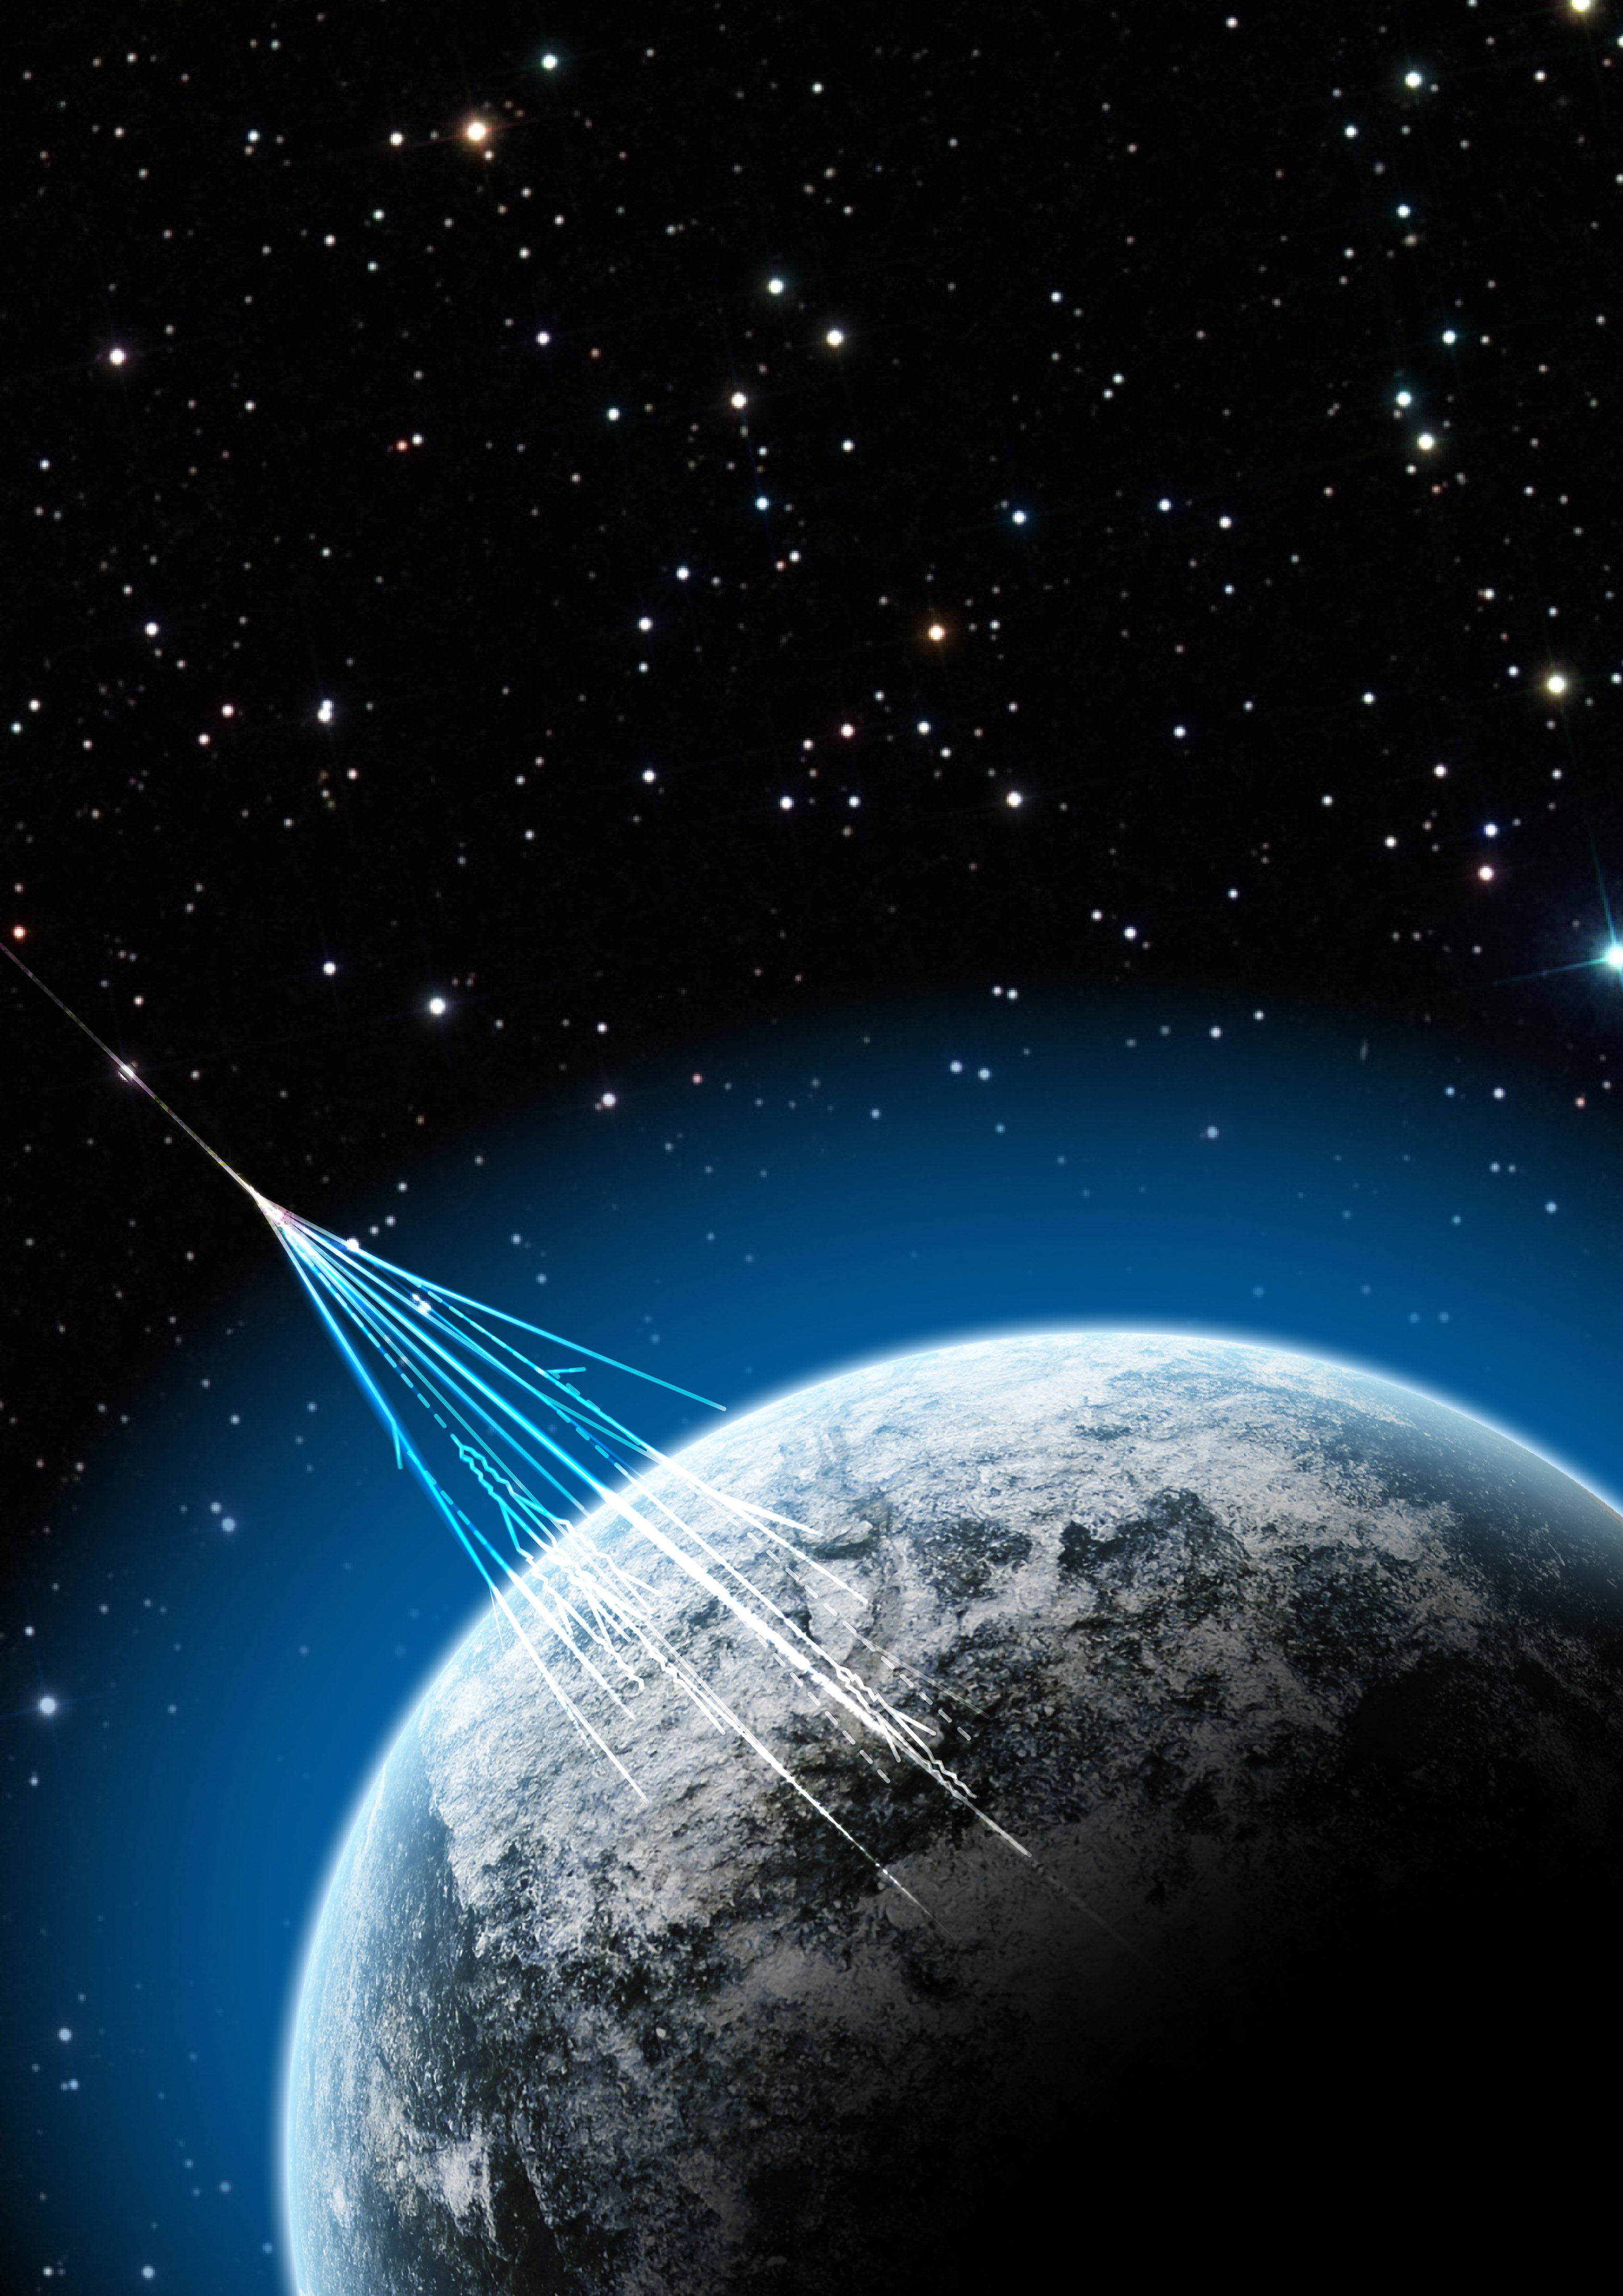
\includegraphics[width=210mm,keepaspectratio]{img/cover.jpg}%
			\vfill
		}%
	}%
}%
\newcommand{\graybox}[3]{%
	\bc\fcolorbox{lightgray}{lightgray!50!white}{%
		\parbox{#1\textwidth}{%
			\bc\parbox{#2\textwidth}{#3}\ec
		}%
	}\ec\par
}
% Fuzz
\hfuzz2pt % Don't bother to report over-full boxes if over-edge is < 2pt
% Listings
\lstset{
	language        = C++,
	breaklines      = true,
	tabsize         = 4,
	frame           = single,
	numbers         = left,
	numberstyle     = \color{gray}\sffamily,
    basicstyle      = \color{violet}\scriptsize\ttfamily,
	keywordstyle    = \color{green!90!black}\bfseries,
	identifierstyle = \color{black},
	commentstyle    = \color{gray}\itshape, % white comments
	stringstyle     = \color{blue},
	showstringspaces= false,
	rulecolor       = \color{lightgray},
	backgroundcolor = \color{lightgray!50!white}
}


\begin{document}

	% Cover and credits -----------------------------------------------------------
	\thispagestyle{empty}
	\pdfbookmark[0]{Cover}{cover}
		\AddToShipoutPicture*{\BackgroundPic}

	\begin{center}

		\vspace*{-2cm}
		\color{white}

		\hrule % --------------------------------------------------------------------------------------

		\huge{\textsc {\textbf{Advanced Experimental Techniques}}}

		\large{\textsc {\textbf{Laboratory of Nuclear and Particle Physics}}}
		\vspace*{2ex}

		\hrule % --------------------------------------------------------------------------------------
		
		 
		\begin{large}
			\color{white}
			\textbf{
				COSMIC RADIATION\\
				\textit{
					Determination of the\\
					hard muon component
				}%
			}%

			\vfill

			April 2005
		\end{large}

		\vspace*{-3cm}

	\end{center}

	\newpage
	\thispagestyle{empty}
	\phantom{hola!}
		
	% Copyright and Credits	
	\null
	\vfill
	\bc
		\begin{minipage}{0.65\textwidth}
			{\sffamily
				\bc
					\textbf{\copyright 2005 \href{https://github.com/me-stevens}{\textbf{me-stevens}}}\\
					\textsc{Creative Commons}\\
					Attribution-NonCommercial 4.0 International\\
					\href{http://creativecommons.org/licenses/by-nc/4.0/legalcode}{(CC BY-NC 4.0)}\\[12pt]
					
\includegraphics{img/license.png}\\[12pt]
				\ec
	
				\small\textbf{Cover image:} Little is known about the ultra high-energy cosmic rays that regularly penetrate the atmosphere. Recent IceCube research rules out the leading theory that they come from Gamma Ray Bursts. (Courtesy: NSF/J. Yang).
			}%
		\end{minipage}\vspace*{1ex}
		\small\href{http://www.interactions.org/cms/?pid=2100&image_no=DE0106}{\textbf{\url{http://www.interactions.org/cms/?pid=2100&image_no=DE0106}}}
	\ec

	\cleardoublepage

	% Table of contents -----------------------------------------------------------
	%    Title aligned right and in italics
	\titleformat{\chapter}[block]{\raggedleft\itshape}{}
		{0pt}{\parbox{\linewidth}{\raggedleft\vspace*{1em}\Huge#1}}
	\pdfbookmark[0]{Contents}{contents}
	\pagenumbering{roman}           % roman page numbering (invisible for empty page style)

	\pagestyle{plain}               % display just page numbers
	\tableofcontents
	\cleardoublepage

		\chapter*{Abstract}

	\textit{This work introduces the students to some properties of cosmic radiation at ground level, in particular, its hard or muon component. First, it shows how to use a wave-guide to determine the working point of two scintillators associated with photomultiplier detectors, obtaining the values V$_\text{threshold}$ ​​= $-$200 mV and HV = 1900 V or HV = 2200 V. It also shows how to determine the value of the time window of the measurement system which has a width of 50 ns.}

	\textit{Making measurements in these working conditions, it is demonstrated that cosmic radiation is statistical in nature and conforms specifically to a Normal or Gaussian distribution. On the other hand, it is possible to separate the contributions of the hard and soft components of the cosmic radiation at ground-level, by making the total flux pass through increasing values of the thickness of lead and aluminium layers of material. Under these conditions, a value ​​of 51 $\pm$ 5 m$^{-2}$s$^{-1}$ is obtained for the hard component of the flux, and 31 $\pm$ 10 m$^{-2}$s$^{-1}$ for the soft component.}

	\textit{Regarding the reliability of the measurements, the effect of the distance between the two scintillators is also evaluated, by calculating the geometric efficiency experimentally and then contrasting the resulting value with the one obtained from a calculation based on a Monte Carlo simulation. These results imply that the system efficiency decreases in proportion to the inverse square of the distance between the detectors.}

	\bfi[H]
		\bc
			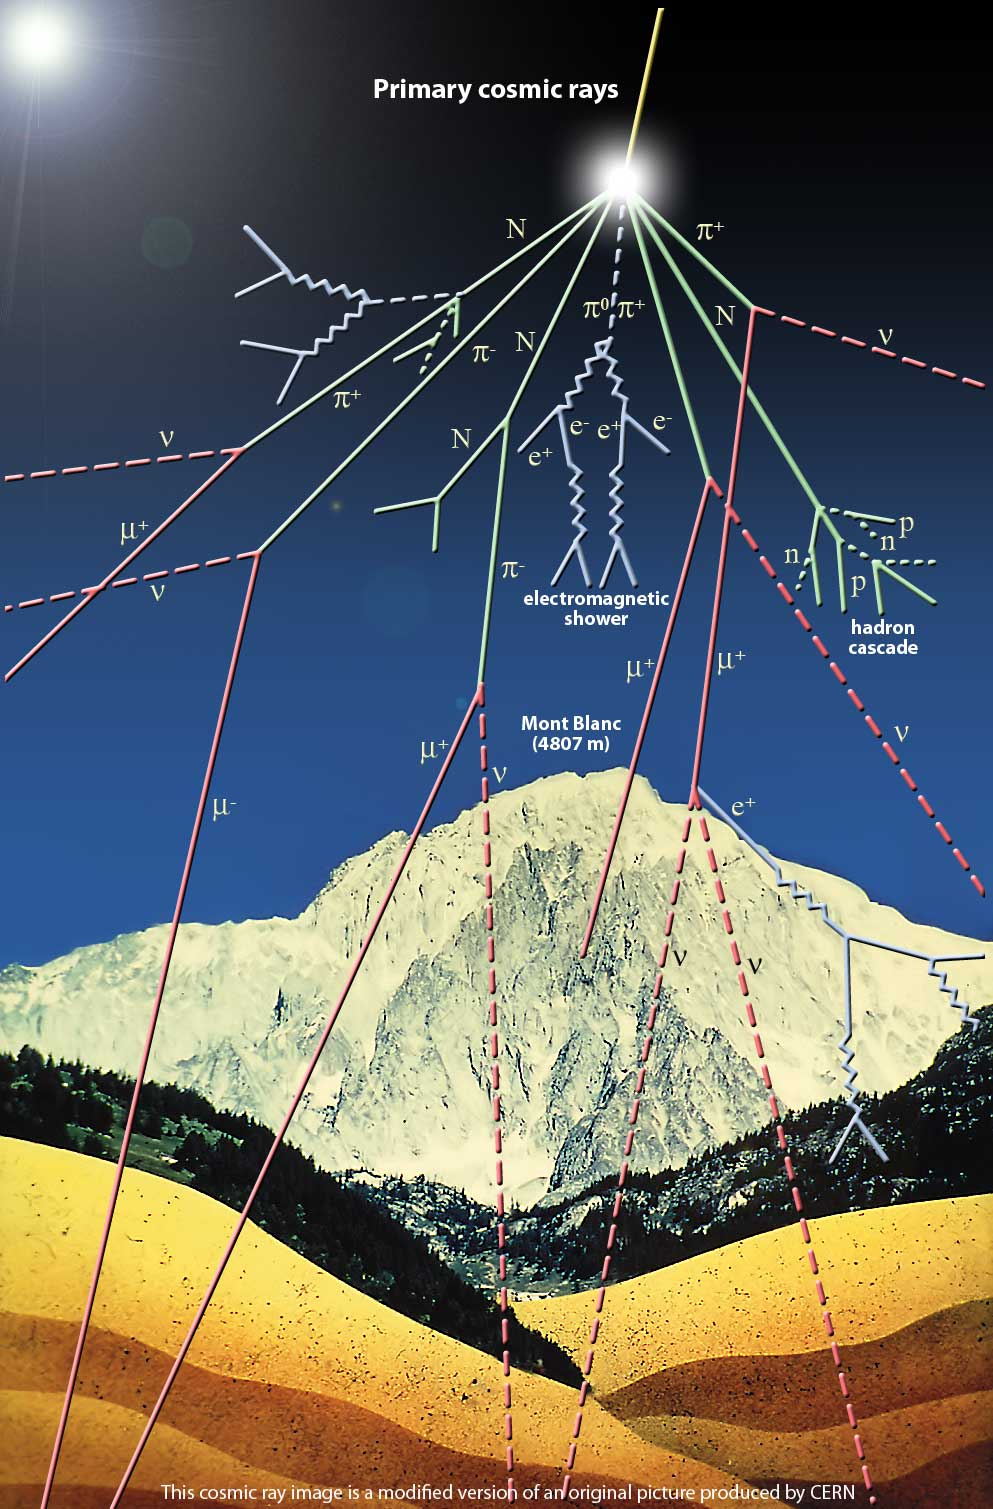
\includegraphics[width=.9\textwidth]{img/cosmic-rays.jpg}\\[12pt]
			\caption
				[Cosmic rays are immensely high-energy radiation, mainly originating outside the Solar System.]
				{Cosmic rays are immensely high-energy radiation, mainly originating outside the Solar System. They may produce showers of secondary particles that penetrate and impact the Earth's atmosphere and sometimes even reach the surface.	(Courtesy: CERN)}
		\ec
		\label{fig:cosmicrays}
	\efi

	\cleardoublepage


	\cleardoublepage

	% Document body ---------------------------------------------------------------
	%	 Title over a yellow background
	\titleformat{\chapter}{\normalfont}{}
		{0pt}
		{\begin{tikzpicture}[remember picture,overlay]
			\node[yshift=-7cm] at (current page.north west)
				{\begin{tikzpicture}[remember picture, overlay]
					\draw[fill=yellow,yellow] (0,-1) rectangle
						(\paperwidth,7cm);
					\node[anchor=west,xshift=2\marginparwidth,yshift=2.5cm,rectangle]
						{\fontsize{380}{130}\color{white}\selectfont\AlegreyaBlack\thechapter};
					\node[anchor=west,xshift=2.5\marginparwidth,yshift=1cm,rectangle]
						{\parbox{\linewidth}{\raggedleft\vspace*{1em}\fontsize{40}{45}\selectfont\AlegreyaBlack#1}};
				 \end{tikzpicture}
				};
		 \end{tikzpicture}
		}
	\titlespacing*{\chapter}{0pt}{100pt}{0pt}

	\pagenumbering{arabic}          % arabic page numbering
	\setcounter{page}{1}            % set page counter
	\pagestyle{maincontentstyle}    % fancy header and footer
		\chapter{Introduction}

	Cosmic rays are highly penetrating high-energy particles (and electro-magnetic radiation), which originate outside the Earth's atmosphere, so they bomb Earth from all directions. Knowing the original composition of the radiation in question is critical, because it provides valuable information not only on the nature of the sources of such radiation, but on its evolution and nuclear synthesis suffered by them.

The interest in the detection of cosmic radiation is very evident since this radiation comes from processes that take place in outer space, typically in the stars, so it is possible to obtain information from these processes from the study of their associated radiation, through the cascades they produce when they enter the atmosphere (a particular case at a global level is the Auger Project).

The study of muon radiation has an absolutely clear interest in the whole framework of particle physics, since it is useful for testing various experimental models, including the \enquote{V-A Theory} of Quantum Field Theory. Furthermore, the attenuation coefficient of the muon is interesting for the design of accelerators, detectors, etc.

The measurements discussed in this work will be performed by the students at the Laboratory of Nuclear Physics, with the equipment available there, under the tutelage of their teacher. These measurements have already been made ​​in the past, so there are results available, which are compared with those obtained here.

In regards to the purely physical part, this work aims to explain how to measure the incident cosmic radiation at ground level, without doing any study in energy (although it is possible too) but rather in intensity (number of particles per unit time). This is due to the fact that with the experimental set-up available, it is not possible to measure the number of hits as a function of the energy of the incident particles, but rather the number of coincidences averaged through all the energies. This task is performed to separate the different components of the incident flux (hard and soft), as did other experimenters. It is intended to show that the values ​​obtained match those tabulated.

Much of the project is dedicated to calibrate the instruments that will be used to make the the measurements, and to set the system into the proper conditions for them. The technique used is one in which two organic scintillation detectors,  placed horizontally, connected to photomultipliers through a light guide, and separated by some distance, are used to take measurements of the coincidences. The advantage of doing so is, that the characteristic noise of these detectors is minimized. Furthermore, solid detectors are used because they have higher densities than gas counters, and give a reasonable probability of absorption for an average size of the detector. The main disadvantage of gas detectors is its low efficiency for many types of radiation of interest in nuclear physics (for example, the range of a 1 MeV gamma ray in air is about 100 m). Our radioactive source is the cosmos, and to filter the components, different thicknesses of lead and aluminium are used.


	This document is divided into several sections. In the theoretical introduction, some basic concepts and terms will be introduced. The experimental part contains a description of the components and the experimental technique as it should ideally be done, although in the Results section the limitations and problems that the student will encounter in practice are presented, as well as the conditions under which the measurements are actually carried out. For completeness, and to give a more linear nature to this guide, four appendices with the more tedious calculations have been included at the end, which will be referenced in the text.


	\graybox{.8}{.65}{
		\bc\textcolor{gray}{\Large{\sffamily Notation used in this document:}}\ec

		\textbf{Abbreviations:}

		EM: electro-magnetic,\\
		UV: ultra-violet,\\
		$\gamma$: gamma-rays,\\
		X: X-rays,\\
		$e^-$: electron,\\
		$\pi$: pion,\\
		$\mu$: muon,\\
		$\nu$: neutrino, etc.\vspace{2ex}

		\textbf{Units:}\\
		International System:\\
		eV: electron volts,\\
		J: Joules,\\
		C: Celsius,\\
		M: mega,\\
		G: giga, etc.\vspace{2ex}

		\textbf{Chemical symbols:}\\
		The elements of the periodic table.\vspace{2ex}

		\textbf{References:}\\
		There are internal (marked in \textcolor{red}{red}) and external (marked in \textcolor{blue}{blue}) references.\vspace{2ex}
	}

		\chapter{Theoretical Introduction}

	\section{Cosmic Rays}

	In the late eighteenth-century, it was of general knowledge that an electroscope\footnote{An \textbf{electroscope} is a device that produces an electric shock due to the cumulative effects of many rays.} slowly loses its charge despite the insulators. In the early twentieth century, many physicists began to investigate this issue. Radioactivity had just been discovered recently, and it was known that it could disintegrate air molecules into positive and negative ions, \textit{i.e.}, into ionized air, which conducts electricity. So, they thought that the slow loss of the electroscope was due to radioactive substances in the earth's crust.

In 1912, \textbf{Victor Francis Hess} jumped into a balloon and was raised up to 5000 m of altitude, where he observed that, the greater the height was, the greater the loss of his electroscope. \textbf{Hess} thought that the mysterious radiation, called \enquote{ultra sharp}, was coming from outside the Earth and was attenuated as it crossed the atmosphere.

\textbf{Robert Andrew Millikan} was the one who in 1927 baptised this radiation with the name \enquote{Cosmic Rays}, thus beginning the boom of their study, aimed at deciphering their nature. This led to the invention of the \textit{Geiger-M{\"u}ller} counter in 1928, which was used for this study, replacing the electroscope, since it can detect each ray  separately. By 1930 the community started using the \textit{cloud chamber} and finally the \textit{photographic emulsion}.



	\section{Nature}

	In studies carried out until 1930, it was discovered that this radiation contains known rays ($\gamma$, X, $e^-$ $\dots$) going at high speed and great energy, as well as other new rays. The experiments revealed a wealth of new particles and high energies, from 1 to 1000 GeV and even $10^{19}$ eV. 

In one particular case, in 1991, the \enquote{\textit{Fly's Eye}}\footnote{Small detectors, each covering a small solid angle, so that each detects only a few photons from the air showers.} observatory at Dugway (Utah) in the U.S. was able to detect particles with energies around 300\e{18} eV, the highest ever recorded energy at the time, equivalent to about 20 J, which would be sufficient to raise 10 $^{\circ}$C the temperature of a tablespoon of water. This energy amounts to $\sim 10^9$ times greater than that achieved so far in manmade accelerators.

We have written this energy as a multiple of $10^{18}$ on purpose, since an energy of $10^{18}$ eV is what is known as the \textbf{Greisen--Zatsepin--Kuzmin barrier}, over which rays can interact with the gammas of background radiation, the Big Bang echo that might have occurred 15\e{9} years ago. It is known that above 7\e{18} eV, $\gamma$ radiation decays, perhaps due to such interaction.

As for particles with energies of 300\e{18} eV mentioned above, they would be less than 100\e{6} years old, so they would not have anything to do with the Big Bang, but could also come from a distant source which were less than 10\e{6} light years from Earth (see \cite{bir:95} for a detailed report on this event and \cite{hal:98} for a review of the highest energy cosmic rays and other references).

	\section{Classification}

	Cosmic radiation is classified in various ways, according to their energy or nature. On the energy side, we can divide it into PRIMARY radiation, which consists mostly of high-energy protons and SECONDARY radiation, which refers to the particle cascades produced by the primary.

According to their nature, they were classified, a bit empirically and a bit following tradition, into HARD and SOFT components, although physicist Werner K. Hei\ss enberg made ​​another classification into four components as follows:

\ben
	\item Soft, composed by $\gamma$ and $e^-$ whose total absorption is achieved with 12 cm. of Lead.
	\item Soft, produced by percussive processes of mesons and their decays.
	\item Hard or penetrating, which is made of fast mesons of different spins and half-lives in the atmosphere produced by the primary proton component. It can contain:
	\item p, n, $\nu$, $\gamma$ and nuclear fragments. This component's intensity continuously decreases at a slower rate than the soft component.
\een

	\section{Showers and cascades}

	Most rays of the atmosphere are secondary radiation. They were discovered by physicist \textbf{Pierre Auger} in 1938. The \enquote{Auger effect} is the emission of an $e^-$ from the extra-nuclear portion of an excited atom when the atom undergoes a transition to a state with a lower excitation energy. It is believed that a human is traversed 20 times per second by showers, causing secondary cascades in bones and tissues.

	\subsection{Latitude effect}

	\bfi[H]		
		\begin{minipage}[s]{0.3\textwidth} 
	    	\bc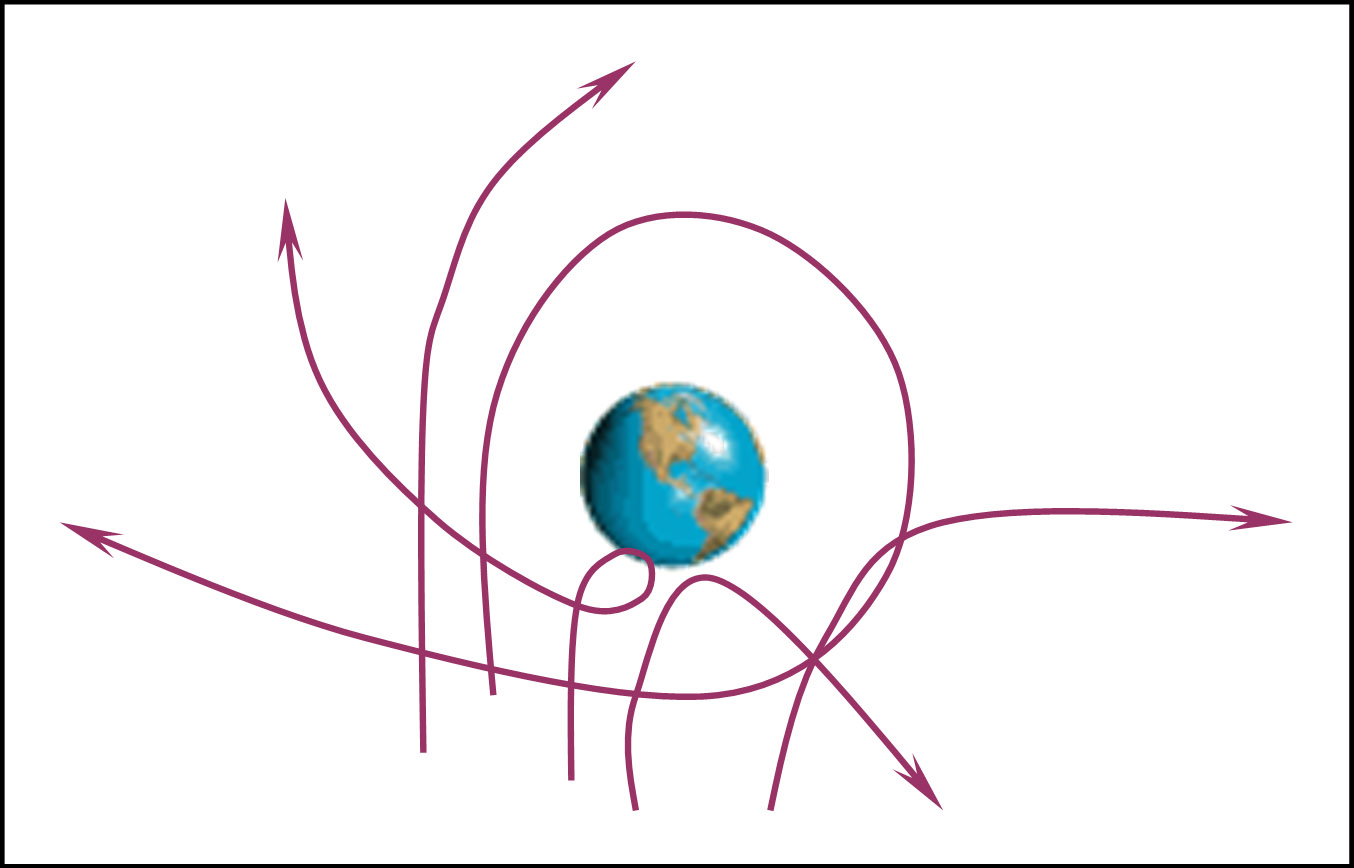
\includegraphics[width=\textwidth]{img/earth.jpg}\ec
		\end{minipage}
		\begin{minipage}[s]{0.7\textwidth} 
      		\captionsetup{width=0.8\textwidth}
			\caption[Earth, viewed from the North Pole.]{Earth, viewed from the North Pole. Effect of the magnetic field of the Earth in the equator on the trajectories of the primary cosmic rays.}\label{fig:earth}
		\end{minipage}
	\efi\captionsetup{width=0.8\textwidth}


	If we were able to study the properties of the primary radiation, it was thanks to the Earth's magnetic field, which bends the trajectories of charged secondary particles. This \enquote{magnetic barrier} is more effective near the equator, and gradually decreases with increasing altitude. Since primary cosmic rays are charged, they (and the secondary) should be more abundant at higher latitudes. This phenomenon is called the \textbf{latitude effect} and led to the discovery that primary rays are charged.

The theory also proves that the positive particles are deflected such that they arrive preferably from Western directions, and negative charged ones from the East. Since the measurements returned higher intensities in the western than in the eastern direction, it follows that the primary particles are mostly positive. So \textit{\textbf{the cosmic radiation varies with latitude and altitude and has an east-west asymmetry}}.


	\subsection{Secondary production process}

	As seen in \ref{fig:earth}, when a primary enters the atmosphere, it collides with an atom, which then decays into secondary cosmic rays, which in turn will decay or continue their path until colliding with another atom.

	Muons are known to be produced by pion decay according to different reactions:

\bc
	\graybox{.4}{.3}{
		$\pi^+ \rightarrow \mu^+ + \nu_\mu$\\
		$\mu^+ \rightarrow e^+ + \nu_\mu + \bar{\nu_e}$
	}

	\graybox{.4}{.3}{
		$\pi^- \rightarrow \mu^- + \nu_\mu$\\
		$\mu^- \rightarrow e^- + \bar{\nu_\mu} + \nu_e$
	}
	\graybox{.4}{.3}{
		{$\pi^0 \rightarrow \gamma + \gamma$}
	}
\ec

	Muons generally do not interact with the atomic nuclei ,and cross the atmosphere (losing about 2 GeV  \cite{eid:04}) until they sink into the earth or disintegrate into electrons. Meanwhile, while $\pi^0$ mesons and those with lower energy than the critical ($\epsilon_\pi$ = 115 GeV) decay immediately, the $\pi^+$ could even collide with other atoms. The phenomenon of \textbf{materialization} can also appear, when the $\gamma$ rays pass near the electric fields of nuclei and \textit{materialize} into electrons in accordance with the reaction: $\gamma \rightarrow e^+$ + $e^-$.

	All these reactions can be seen in Fig. \ref{fig:cascades}.

    \bfi[H]
      \bc
      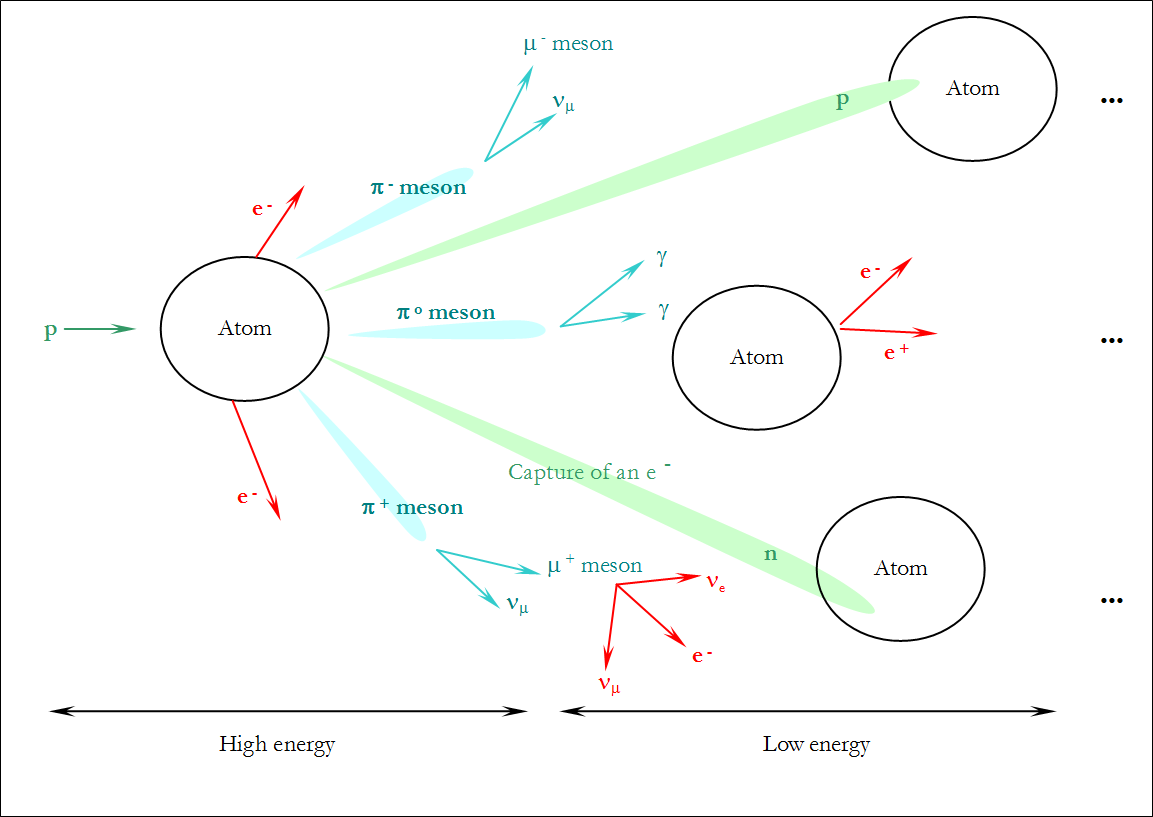
\includegraphics[width=14cm]{img/cascades.png}\\[12pt]
      \caption[Production of secondaries in Earth's atmosphere.]{Rough picture of the production of secondary in Earth's atmosphere, where the waterfall is produced by a 20 GeV proton at an altitude of 16 km.}\label{fig:cascades}
      \ec
    \efi


	All these particles from a cascade produced by a primary particle can reach the ground simultaneously, covering large hectares. Depending on the energy of these primary incident particles, more or less secondaries are produced:

	\bi
		\item If $E \geq 10^6$ GeV, $\sim 10^5$ secondary particles  are produced.
		\item If $E \geq 600\e{6}$ GeV, $\sim 10^8$ secondary particles are produced.
	\ei

These cascades can be described by a set of coupled equations and Monte Carlo simulations, but can also be approximated analytically in certain energy ranges. For example, the primary nucleons intensity per nucleon energy (E) in the energy range of GeV to $10^2$ TeV can be approximated by the expression:

	\be\label{eq:in} I_N(E) = 1.8 E^\alpha nucleon/ cm^2GeV\ee


where $\alpha$ is the differential spectral index of the cosmic-ray flux and has a value of 2.7.
Furthermore, the vertical intensity of nucleons after crossing an atmospheric thickness X in gcm$^{-2}$ is given by \cite{eid:04}:

	\be\label{eq:in2} I_N(E, X) \approx I_N (E, 0)e^{\frac{-X}{\Lambda}} \ee

where $\Lambda$ is the mass absorption coefficient that gives an idea of ​​the range of nucleons in air, while the corresponding expression for pions with energies much lower than the critical ($\epsilon_\pi$) is \cite{eid:04}:

	\be\label{eq:ipi} I_\pi(E_\pi, X) \approx \frac{Z_{N\pi}}{\lambda_N}I_N (E_\pi, 0)e^{\frac{-X}{\Lambda}}\frac{XE_\pi}{\epsilon_\pi}\ee


where the $Z_{N\pi}$ factor has to do with the distribution of charged pions in interactions of nucleons with nuclei of the atmosphere. This expression has a maximum at 15 Km of altitude.

In the case of the soft component, the most common electromagnetic cascades can be of two types, \textit{bremmstrahlung} and pair production.

However, at sea level, the most abundant secondary particles are muons. Energy and angular distribution are given by a convolution of the spectrum of production, energy loss into the atmosphere and the decay\footnote{For example, 2.4 GeV muons would travel 15 Km in the atmosphere before decaying, but this distance is reduced to 8.7 Km due to energy losses.}. Their average energy in the ground is about 4 GeV, for which the angular distribution is proportional to $cos^2\theta$.



	\section{Origin}

	Their origin is still being studied. Some observations:

	\bi
		\item The intensity of the cascades increases with solar perturbations, electromagnetic high frequency radiation emitted by the Sun contributes to the radiation reaching us. The remaining particles from outside the Solar System are modulated by the solar wind, which slows and excludes the rays of lower energy (<10 GeV) from the initial beam \cite{eid:04}.

		\item They are believed to be a remnant of some supernovae in our galaxy. However, higher energy rays would originate outside the Milky Way.

		\item It is thought that cosmic rays are trapped in the magnetic field of the galactic system for periods of 1 to several million years, causing energy densities $\sim$ 1 eV / cm$^3$ (approximately the energy of the magnetic field of the Sun). This capture increases radiation intensity, and explains why they arrive in equal numbers in all directions of the sky.

		\item The primary radiation is very different from what it was originally. Looking at Table \ref{tab:composition}, if we compare the composition of the radiation with the radiation of many stars, we see that is favoured in heavy elements and poor in the light ones, so they must have originated from the stars whose evolution is more advanced.
	\ei


    \ctable [
	cap     = {Composition of the Cosmic rays.},
 	caption = {Composition of the Cosmic rays.},
 	label   = {tab:composition},
	width   = 0.5\textwidth,
 	pos     = H,
	]
	{		r				D{.}{.}{5.4}      }{}
 	{\FL
         	H (p)			& 91.7\\
         	He ($\alpha$ particles)	& 7.6\\
         	Li, B, Be		& 0.13\\
         	C, N, O, F		& 0.35\\
         	Z > 10 			& 0.22
    \LL}


	\chapter{Experiment}\label{chap:exp}


\section{Set up and instrumentation}

For this measurements, the students will have these materials available at the Laboratory of Nuclear Physics:
	\bi
		\item Scintillators and photomultipliers
		\item Acquisition electronics:
		\bi
			\item Pre-amplifier and amplifier
			\item Scope
			\item Pulse Generator
			\item High voltage power supply
			\item Discriminator
			\item Coincidences module
		\ei
		\item Blocks and layers of absorbent materials
		\item Voltmeters
		\item Wiring
	\ei

	\bfi[H]
		\bc
			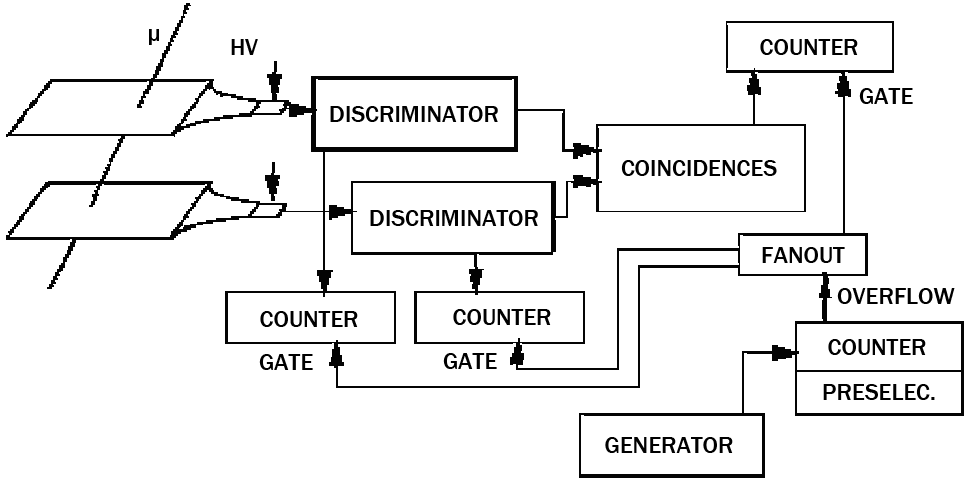
\includegraphics[width=\textwidth]{img/setup.png}\\[12pt]
			\caption[Experimental set up.]{Experimental set up.}\label{fig:setup}
		\ec
	\efi



	\subsection{Scintillators and photomultipliers}

		\subsubsection{Scintillators:} 

			\underline{\textit{Characteristics of the detectors used:}}

			The detectors chosen for this application must be able to withstand a large electric field, and in the absence of radiation, the electric current flow should be minimal or null so that the noise is low. This seems to require an insulating material, but also the e$^-$ should be easily extracted from the atoms, and in great number by the radiation. Also, the  ions must be able to easily travel in the material, which suggests using an electrical \textbf{conductor}. The obvious compromise is what we found in the laboratory: \textbf{a semiconductor}.

There are two basic types of detectors, those composed of \textit{organic} materials (which may be liquid or solid), and those made of \textit{inorganic} materials. The choice of one or the other depends on the type of experiment to be performed. In this case we are looking for a short response time, so the relatively inefficient plastic scintillators are a better choice. In this experiment we have chosen \textbf{organic solid plastic scintillators}.

The properties considered in choosing the material include:

		\bi
			\item \textit{the fraction of incident energy that appears as light}: they can be used in a wide range of energies from 20 keV (e$^-$) to 200 MeV (heavy ions),
			\item \textit{the efficiency} (the probability that the radiation is absorbed) for the active area, the efficiency is 100\%, and its power vs. pulse-height curves are linear over a wide range,
			\item \textit{the response time}: fast pulses emerge and are suitable for short times ($\sim$ 1 ns) with coincidences circuitry,
			\item \textit{the energy resolution}: it is only surpassed by the spectrometers,
			\item \textit{the transparency}: the scintillators are transparent to its own radiation.
		\ei

The dimensions of these scintillators in the laboratory are listed below:

		\bc \textit{\textbf{S}} = (31 cm.) $\times$ (10 cm.) = \textbf{0.031 m$^2$}.\ec

Whenever a reference is made to \textit{\textbf{S}} in this work, this values will be used.

			\noindent\underline{\textit{Operation:}}

In scintillator counters, electrons formed in the ionization process are the same as those of the electronic pulse. The intermediary between the two is the ordinary light.

In organic scintillators, interactions between molecules are weak, and its properties can be understand in terms of discrete excited states of molecules. The electrons can be excited to higher electronic states (jumps between electronic levels) or the atoms of the molecule may start vibrating (jumps between vibrational levels). Typical vibrational energies are of the order of 0.1 eV, whereas the electronic excitation energies are on the order of eV.

		\noindent\begin{minipage}{0.5\textwidth} 
			\hspace*{2ex} The excited electrons are those that are not involved in the binding of the molecule. The incident cosmic radiation interacts with many molecules, losing a few eV (slightly different for hard or soft) in each interaction, exciting them.\\

			\hspace*{2ex} The vibrational states excited with that energy first decay ($\sim$1ps) to the first vibrational ground state of the excited electronic state, which then decays ($\sim$10ns) to one of the vibrational states of the electronic ground state, which in turn decays quickly to its corresponding vibrational ground state.
		\end{minipage}
		\begin{minipage}{0.5\textwidth} 
			\bfi[H]
				\bc
					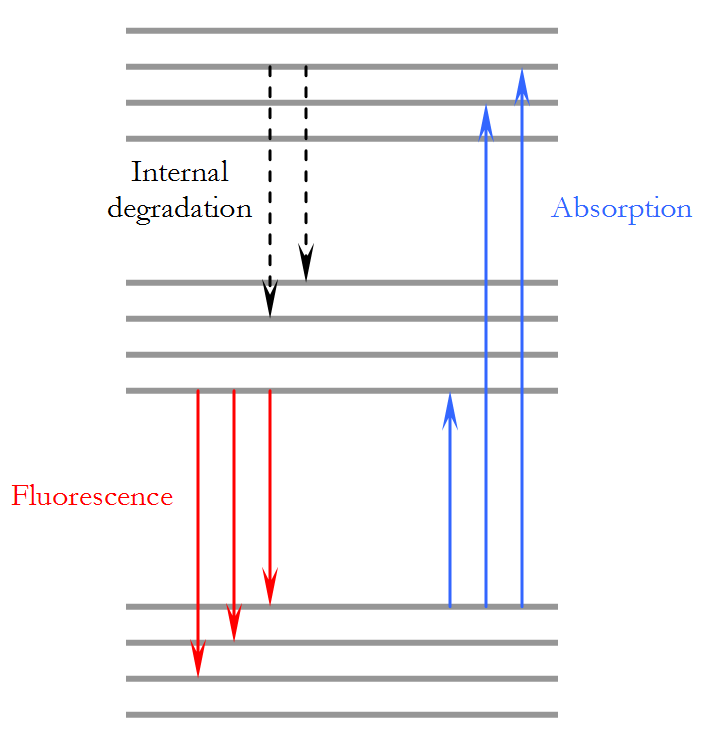
\includegraphics[width=.9\textwidth]{img/scintillator.png}
					\label{fig:molecular}
				\ec
				\caption[Molecular gamma decay.]{Molecular gamma decay.}
			\efi
		\end{minipage}\captionsetup{width=0.8\textwidth}


These transitions can be radiative or non-radiative. In non-radiative, there is light emission (luminescence), which in the case of atoms is around the UV.

Finally, this explains its \textit{transparency}: Under normal circumstances, at room temperature, all of the scintillator molecules are in the lowest vibrational state of the electronic ground state.

At thermal energy (kT = 0.025 eV) the corresponding population follows a \textbf{Boltzmann distribution}: \textit{exp($-$E / kT)}, so it is very unlikely that there are any excited vibrational states at that temperature. This ensures that ONLY ONE of the photons emitted in the many possible transitions has a probability of being absorbed by the scintillator itself.

There are also other processes happening within a scintillator:

	\bi
		\item \textit{Fluorescence Emission} of radiation of a given wavelength by a substance as a result of the absorption of radiation of a shorter wave length. This emission occurs essentially only during irradiation.

		\item \textit{Pair production}: A process for X-radiation and $\gamma$ absorption in which the incident photon is annihilated in the vicinity of the absorbent nucleus of the atom with the subsequent production of a pair e$^-$ / e$^+$. This reaction only occurs for incident photons whose energy exceeds 1.02 MeV.

		\item \textit{Photoelectric Effect}: A process by which a photon removes an e$^-$ of an atom. All the energy of the photon is absorbed in extracting it and giving it kinetic energy.

		\item \textit{Compton effect}: An attenuation process observed for X or $\gamma$ radiation, in which an incident photon interacts with an orbital e$^-$ of an atom to produce a recoil e$^-$ and a scattered photon of lower energy than the incident.
	\ei

		\subsubsection{Photomultipliers (PM):}

		For this experiment, the geometry of the photomultiplier is very different from the geometry of the scintillators. This justifies the use of a light guide between the two.

		The gain of a PM is calculated as:

		\be\frac{number\ of\  e^-\  going\  out}{number\  of\  e^-\  going\ in} \sim 3-4\ee

At the end of \textbf{n} stages, the number of e$^-$ will be N (e$^-$) \textbf{$\sim$ 4$^n$}.

		In the semitransparent photo-cathode, the incident radiation extracts an e$^-$ by photoelectric effect. The photo-cathode is a thin layer of photosensitive material with a work function $\phi$, so that if the frequency of the incident photon is $\nu$, the e$^-$ will exit with an energy of:

	\bc$E = h\nu - \phi$\ec

From this expression it is evident that a minimum $\nu$ is needed for the process to happen. PM quantum efficiency is then defined as:

	\be QE(\lambda) = \frac{photoe^-\ out}{incident\ gammas}\ee

which depends on $\lambda$ and the structure of the material.

		Then they pass through the e$^-$ collector, where there are several focusing electrodes that use an electric field to attract the e$^-$ to the first dynode. This way, the number of e$^-$ reach the dynode from any point of the cathode, and the arrival time is independent of the emission point.

		In the tube of the PM, the e$^-$ are accelerated into a series of secondary electrodes, generating more e$^-$ in each new clash with the dynodes. These are connected to a high voltage source and a series of voltage dividers. Thus, typical potential differences of about 100 V between adjacent dynodes are obtained, and therefore, the electrons impact the dynodes with about 100 eV of energy.

	\bfi[H]
		\bc
			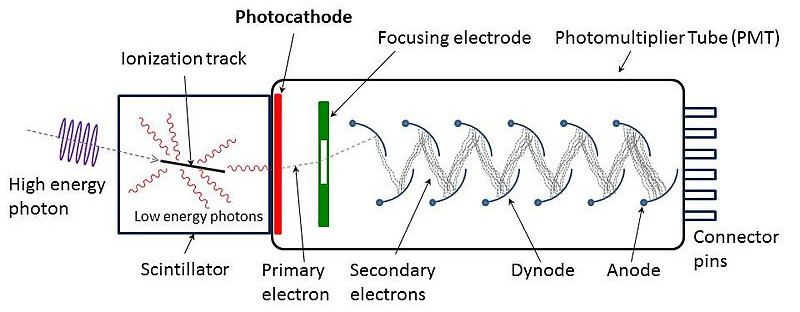
\includegraphics[width=\textwidth]{img/pmtube.jpg}\\[12pt]
			\caption[Schematic view of a photomultiplier.]{Schematic view of a photomultiplier. The electrons released from the cathode are attracted to the first dynode and multiplied. Each successive dynode is at a higher potential than the previous. A typical tube has 10 to 14 dynodes. At each step, the number of electrons is increased by a factor of about 5. \textbf{Image credit:} By Qwerty123uiop (Own work) [CC-BY-SA-3.0 (\scriptsize\href{http://creativecommons.org/licenses/by-sa/3.0}{\textbf{\url{http://creativecommons.org/licenses/by-sa/3.0}}}{\small)], via Wikimedia Commons.}}\label{fig:pmtube}
		\ec
	\efi

The dynodes are made ​​of a material that has a high probability of emitting secondary electrons. Between $10^5$ and $10^7$ e$^-$ are created by each photoe$^-$ emitted by the cathode, and to free an e$^-$ can cost up to 2 or 3 eV. A gain of 30--50 e$^-$ is therefore possible. The amplification depends on the number of dynodes (n) and the voltage between them (V$_{d-d}$).
 
The secondary emission factor is defined as $\delta = k\Delta V_{d-d}$, so the gain will be $G = \delta^n$. Keep in mind that changes of 1\% in $\Delta V_{d-d}$ lead to changes in gain of n\%, which means that HV has to be regulated.

		However, electrons are released in random directions in the material, and relatively few will be actually delivered to the surface, so that a gain of 5 in each dynode is more common. Even so, with a tube 10 dynodes, the total gain will be of 510 ($\sim$107). That is, each time a cosmic ray hits the system, it produces 10,000 \enquote{primary} ionizations in the scintillator, of which about 100 are gammas.

Finally, the cascade of e$^-$ is collected at the anode, and becomes a signal of electric current that can be amplified and analysed.
	   
		When connecting an oscilloscope to a PM in the set up that we have in the laboratory, it will be noted that there is always a \enquote{dark current}, due to the presence of neutrinos, decays at room temperature, etc. Furthermore, with the increase in the threshold voltage of the discriminator, the noise and signal amplitude will increase too.

The joint of the scintillator to the PM is usually done through an optical coupling (silicone oil, light guides, etc.). If we connect a scintillator to a PM, a signal with a pulse of a certain amplitude that appears randomly will be added, this means that a particle has reached the scintillator. In addition, the noise that it had before will be increased by the so-called \enquote{white noise}, which has a flat spectrum and is nothing but the noise of the signal itself. Parasitic currents can appear also. As the voltage (HV) increases, the gain will increase too, and therefore the number of events, but there will come a time when even if the tension rises, no more particles are detected, only noise will be increased.

	\noindent\underline{\textit{Detection process:}}

To summarize, the detection process follows these steps:

	\ben
		\item The incident cosmic radiation interacts with atoms and molecules, exciting the material.
		\item The excited states decay emitting visible (or near visible) light, or fluorescence light.
		\item The light travels through the light guides, and reaches the photosensitive surface of the PM, extracting photoelectrons.
		\item The electrons are accelerated and multiplied, to form an electrical pulse in the photomultiplier tube.
	\een


	\subsection{Acquisition Electronics}

In this measurements, a chassis with rear power supply adapted for NIM (\textit{Nuclear Instrument Module standardized}) modules was used, following the AEC Report TID-20893 standard, which ensures compatibility in size, power and signal level for instruments manufactured by different vendors.

The system for this experiment is already assembled, and includes a set of modules that are used in many experiments: a pre-amplifier, an amplifier, a discriminator, a counter and an oscilloscope. Each module provides a necessary function for the overall system, which according to the diagram in Fig. \ref{fig:setup} is nothing more than a simple \textbf{counting system}. It is important that all the equipment has the same impedance, to avoid signal reflections.

These electronic modules are divided into two general types:

	\bi
		\item \textit{Logic}: Those that generate an output pulse of fixed shape and amplitude if a logical criterion is fulfilled. \textit{Example}: the discriminator, which provides an output pulse (always with the same amplitude) each time it receives an input pulse whose amplitude is greater than the threshold level. The SCA is also logical.

		\item \textit{Linear}: Those in which the linear output signal contains information such as the energy of a detected event (one incident particle that has been absorbed in the detector). The linear signals vary over a range of amplitudes which shows the energy spectrum analysis of the event.
	\ei

It is always important to distinguish between linear and logical connections to mount a NIM equipment. The logic signals are often used to provide timing information and control the function of each instrument in a system.

		\subsubsection{Preamplifier and amplifier:}

Particles produce pulses from the detector whose amplitudes are proportional to the energy of cosmic radiation. The \textbf{preamplifier} and \textbf{amplifier} simply amplify each pulse by a fixed gain factor, and shape the pulse as well.

For example, with a gain factor of 10, if a particle arrives with 5 MeV, a signal of 0.5 V will leave the preamplifier, and a signal of 5 V from the amplifier. So each time a particle of 5 MeV hits the detector, a pulse of 5 V is produced.

The linear signal is the output of the amplifier, and contains information on the energy of the particle that produced the pulse, \textit{i.e.}, the output of the amplifier is proportional to the energy of the absorbed particle. 

		\subsubsection{Discriminator:}


In addition to the information provided by the pulse height, the number of linear signals can also show how many events occurred with a certain pulse amplitude per unit time. If the discriminator is set to 5.1 V for the output of the amplifier, and particles are coming with energies of 5 and 6 MeV, the logical pulse discriminator sends only the particles of 6 MeV. These logic pulses are then sent to the counter and counted.

		\subsubsection{Oscilloscope:}

It is the instrument used to observe the input and output pulses for the modules in the system, and to determine whether the shape of the signals, the amplitudes and timing are correct with respect to the rest of the equipment.

	\bfi[H]
		\noindent\begin{minipage}{0.5\textwidth} 
			\bc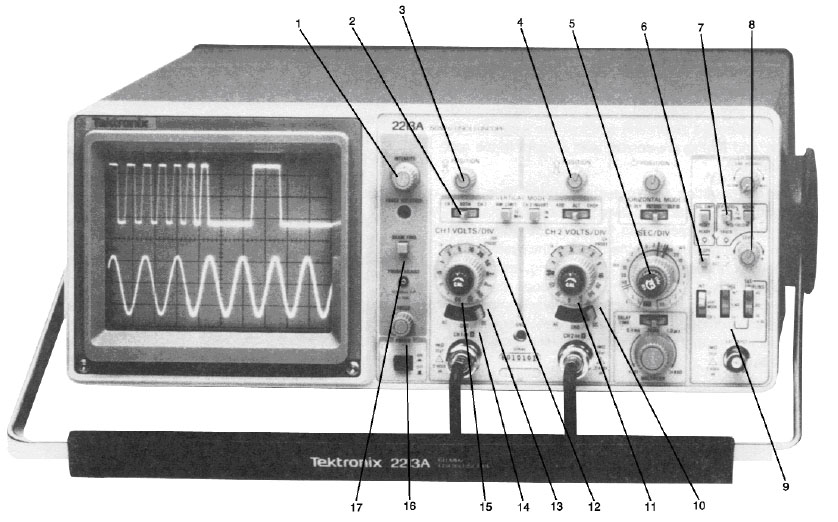
\includegraphics[width=.9\textwidth]{img/scope.jpg}\ec
		\end{minipage}
		\begin{minipage}{0.5\textwidth} 
			\captionsetup{width=0.8\textwidth}
			\caption[Image of a conventional oscilloscope.]{Image of a conventional oscilloscope.}\label{fig:scope}
		\end{minipage}\captionsetup{width=0.8\textwidth}
	\efi

		\subsubsection{Pulse Generator:}

This instrument simulates the pulses generated in the radiation detector and supplies the pulses with the known characteristics to the system entry. It is used for calibration, synchronization, etc. If used together, the oscilloscope and generator ensures that the electronics have been assembled according to the requirements of the experiment.

		\subsubsection{Discriminator:}

When a cosmic particle reaches the detector, the former will get mixed with the noise of the latter. Therefore, the signals output by both PMs must be filtered, by passing them through the \textbf{discriminator module}, where it will be required that the amplitude exceeds a certain threshold, in order to separate the produced particles that deposit more energy, such as the cosmic muons.

The module that performs this task is the discriminator, which accepts an analogue signal as input, whose amplitude and duration are dependent of the process that took place in the detector. The discriminator's output will be a logic signal with fixed height and duration (50 ns), and a rectangular shape, if the input signal has exceeded the discriminator's threshold. Each discriminator has two outputs: one is used to feed a counter that lets us know the number of pulses from each photomultiplier, and the other will address the coincidences module.

		\subsubsection{Coincidences module:}

The coincidences between the two detectors are evaluated using a NIM coincidence unit. This module has several inputs and one output. We will have an output signal when the input pulses overlap in time at least partially. Taking the output of this module to another counter we can accumulate the number of matches in a space of time.


		\subsubsection{Blocks and layers of absorbent material:}

There is a total of 20 layers of Al and 9 layers of Pb, with a thickness of 1.5 mm each.  The layers are not perfectly flat but can be bent. The Pb blocks are 5 cm thick.


		\subsection{Voltmeters}

The voltmeters used in the laboratory have a sensitivity of three and a half digits. They will be used to measure the voltage (HV) and the threshold voltage $V_{threshold}$. Therefore the error in measuring these quantities depends on the measurement scale used in each case [Appendix \ref{chap:app3}]. To measure, the value of the voltage is adjusted by turning a screw (potentiometer) and placing the terminal of the voltmeter to the corresponding measuring point. The proportionality constant of the voltmeter (which has a value of $\sqrt{2}$ since it measures effective values), ​​must also be considered.


		\subsection{Wiring}

Connections between linear and logic signals are made via standard BNC coaxial cables and connectors. The cables used to connect the two detectors with the coincidences module were of the same length so that the signal delay should be the same.


		\section{Determination of the working point}

To determine the operating point, the zone of maximum efficiency and stability of scintillators is searched. Once it is done for one, it is known for the other, since they are very similar. The high voltage (HV) and the threshold of the discriminator must be  properly adjusted.

	\graybox{1}{.9}{%
		\begin{description}
			\item[Problem] \hfill \\
				We want to detect the particles that have crossed both scintillators, any other signal is noise. This leads to the problem of determining the appropriate time window\footnote{In our case it corresponds to the time it takes a particle to travel the distance between the two scintillators.} of the detection system.
			\item[Solution:] \hfill \\
				To do this, we first have to know how fast the particles we want to detect travel. Muons, for example, are relativistic at ground level according to \cite{eid:04}. Since the distance between scintillators is $\sim$cm, this gives us a time window of  $\sim$ ns.
		\end{description}
		}

Since the total flux of cosmic rays at ground level is $J = 180 cm^{-2}s^{-1}$, the time window becomes: $\Delta T \ll 0.15 s$, as is calculated below. This gives an estimate of its value; but it is possible to determine it experimentally, defining:

	\be\label{eq:Qs} Q[s] = \frac{1}{2}\frac{N_{coinc}/t}{(N_1/t)(N_2/t)} \ee

It is found that when the number of counts is high, $Q = \Delta T$.


The value of the voltage is set to less than that recommended by the manufacturer for both scintillators, and the highest possible value for the discriminator is chosen. Measurements are taken sweeping the interval 1700--2300V in steps of 100V with one of the scintillators. $Q$ is calculated according to the above expression, and it is plotted against HV, where it is clear than it tends asymptotically to the value of the time window. This value is compared with the previous calculation.


	\subsection{Estimation of spurious coincidences}

	\graybox{1}{.9}{%
		\begin{description}
			\item[Issue:] \hfill \\
				Although the time window may be well adjusted, it is possible that randomly, two different particles arrive each at a different detector inside the time  window (or that the noise in both detectors generates a coincidence) and then the system will assume it as a real coincidence.
			\item[Solution:] \hfill \\
				The frequency of random coincidence events is proportional to the coincidences window size and to the number of individual counts on each detector, \textit{i.e.}:

\noindent\be Random\ coincidences: \frac{N_{rand}}{t} = \frac{N_1}{t}\frac{N_2}{t}2\Delta T\label{eq:random}\ee
		\end{description}
	}

Once the time window is determined, the spurious contribution can be obtained making this simple calculation.

With the flux $J$ obtained at ground level, if $S$ is the surface of the detector, the average rate of particles in each detector is given by $N / t = J · S$ = 180 $m^{-2}s^{-1}\times$0.031$m^{-2}$ = 6 particles per second. If it is imperative that $N_{rand} / t \ll N / t$, and the above expression is used, we obtain $\Delta T \ll 0.15 s$, as discussed above.


	\subsection{Determination of the plateau by changing the high voltage}

	\fcolorbox{lightgray}{lightgray!50!white}{
		\parbox{\textwidth}{

			\bc\parbox{.9\textwidth}{
	\begin{description}
		\item[Issue:] \hfill \\ The detector does not behave the same way for all voltages. If the HV voltage is very small, the signal strength is small and falls below the threshold, so it is not registered. If the HV is high, we have a considerable contribution of detector noise (see \enquote{\textit{	Set up and instrumentation: Scintillators and photomultipliers}}). What we want is an intermediate situation.
		\item[Solution:] \hfill \\ Several measurements are realized between 1700 and 2300 HV V as in the previous section. Initially the thresholds are set to their minimum values ​​(-35 mV), so that all the signals from the detectors are received. Then the signals from each detector and the coincidences are noted. As the noise is expected to be high, it is expected that the number of counts of each detector (ray + noise) will be greater than the number of coincidences (rays).
	\end{description}
			}\ec
		}%
	} \par



If the coincidences are plotted against the HV, a substantially constant, flat area called \textit{plateau} will appear, which allow us to determine the operating point of the detectors. If random coincidences are also included in the same graph, there will be another curve that will give us information on the voltage at which these coincidences start contributing.


	\subsection{Determination of the plateau by changing the threshold}

The operating voltage is set to the manufacturer's recommended value,  and the threshold is set to the maximum ($-$400 mV). Then it is reduced  in steps of 50 mV until the minimum is reached ($-$35 mV). By raising the detector's threshold, a reduction in the difference between the number of coincidences and individual signals must be observed, because noise is mainly discriminated.

	\section{Statistical characterization of cosmic radiation}

According to the theory of probability, if a distribution function is known, every moment of it is known too. Conversely, if a distribution of all moments are known, this is equivalent to knowing the distribution. Therefore to determine a probability distribution associated with an experiment, there are two alternatives: either to determine the distribution or to determine all its moments (or at least the most relevant).

When the number of occurrences of a measure is very small, the probability distribution fits well to a Poisson distribution (Appendix \ref{sec:poisson}). Radioactive decay (in the present case, the primary particles decaying into the secondary, which are the ones of interest here) is a random process that obeys the Poisson distribution, according to which the standard deviation of the distribution with media $\mu$ is $\sqrt{\mu}$ (Appendix \ref{sec:poisson}).

However, when the number of counts is greater, data starts to progressively conform to a Gaussian distribution. Therefore, the procedure is to make measurements in intervals of 5s for one hour, to have something of the order of about 3 counts, and then repeat the same measurement every 10s and 20s. With the values ​​obtained, a histogram of the number of coincidences counted in each measure is plotted. Then it is found that the data represented in the histogram follows a Poisson distribution in the first case, while in the second and third case it follows a Gaussian distribution. The goodness of fit is evaluated with a $\chi^2$ test.


	\subsection{Modelling of the quality of experimental data and settings: Chi square test}

Through the minimization process known as the \textit{least squares method}, we can determine the value of a theoretical parameter function $f(x, a_1, ..., a_m)$ which is fitted to a set of $n$ experimental points $f (x_i; y_i)$.

The method states that the best values ​​of the $a_j$ are those for which the function


	\be\chi^2 = \sum_i^n\frac{\left(y_i-f(x_i;a_j)\right)^2}{\sigma_i^2}\ee

is minimal, which is usually calculated by numerical methods.

Suppose a set of $n$ random events that follow Poisson and Gauss and appear with frequencies $e_i$. Let $N = \sum e_i$ be the number of expected frequencies. Then the probability of observing the event $i$ is $e_i/N$, and it represents the fraction of cases in which we would see it if we repeated the experiment infinite times. Thus we obtain:

			\noindent\be\chi^2 = \sum_i^n\frac{\left(o_i-e_i\right)^2}{e_i}\ee

where $e_i$ are the theoretical frequencies and $o_i$ are the experimental ones.

Limitation: If all $o_i$ are greater than $e_i$ is not possible to say that the agreement is very good even if $\chi^2$ is small. This method is not a universal panacea.

The procedure is as follows: the number of events occurring in each area of probability is compared with the number of expected events. If the difference is small (of the order of the expected fluctuations, i.e., $\sim \sqrt{e_i} = \sigma_i$), there is a good agreement between experimental and theoretical data (Appendix \ref{sec:chi2}), i.e., if $\chi^2 < \nu$ there is agreement, and if $\chi^2 \gg \nu$, there is not, where $\nu$ represents the degrees of freedom of the system.



\subsection{Separation of the hard component of coincidences}\label{sub:separation}


Recalling the equations \ref{eq:in}, \ref{eq:in2} and \ref{eq:ipi} in the  theoretical introduction chapter, we see that each particle is attenuated differently in the atmosphere depending on their energy.

With our experimental set-up we can not measure the number of coincidences as a function of energy, but we measure the number of coincidences averaged over all energies. However, with the help of the oscilloscope and without altering anything, we could determine the energy distribution of the incident particles, simply by connecting the detector to the oscilloscope and measuring the amplitude of the signals appearing (for this you may want to freeze the image in the oscilloscope with many reflections).

Some definitions are important here:

\bi
	\item \textit{Linear absorption coefficient} ($\mu$): variable indicating the ability of a material as an absorber. In g cm$^{-2}$.
	\item \textit{Mass absorption coefficient ($\Lambda$)}: The linear absorption coefficient divided by the density ($\rho$) of the absorbent in g cm$^{-3}$ is often expressed as $\mu / \rho$ and units are usually given in cm.
	\item \textit{Stopping power ($dE / dx$)}: Measurement of the effect of a substance on the kinetic energy of a charged particle passing through. It is typically given in MeV / cm.
\ei


It also important to introduce the typical exponential decay law: given a certain flux of particles with a certain kinetic energy, the number of them passing through a material of increasing thickness typically follows an exponential decay function given by:

		
		\be-\frac{dN(x)}{dx} = \mu N(x) \quad \rightarrow \quad \int_{N_0}^{N(x)}\frac{dN(x')}{N(x')} = - \mu\int_0^x dx' \ee
		\bc $N(x) = N(0) e^{-\mu x}$ \ec
		\be N(x) = N(0) e^{\frac{-x\rho}{\Lambda}}\ee

where $N(x)$ is the number of particles of the incident beam that \enquote{survive} at a depth $x$ of the material, $\mu$ is the \enquote{coefficient of linear absorption} of such particles in the material, and $N (0)$ is the number of particles that hit the material initially.

Since $\Lambda$ is a characteristic parameter of the radiation, the attenuation coefficient depends on the particle type; given a particular material, the absorption coefficient $\mu$ is smaller in the case of muons than in the case of the soft component, because $\Lambda$ is greater.

As in air it would be difficult to stop them with the measurement system used\footnote{In air the values ​​are: $\Lambda_{soft}$ = 100 g cm$^{-2}$ and $\Lambda_{hard}$ = 1500 g cm$^{-2}$, which give typical values ​​of 150 Km for muons in air, and 10 km for electrons.}, higher intensities are mitigated with elements such as Pb and Al:

\bc$\rho_\text{Pb}$ = 11.340 g cm$^{-3}$\\[12pt]
  $\rho_\text{Al}$  = 2.700 g cm$^{-3}$\ec

The procedure is as follows: the Al plates are placed between the two scintillators and then the number of layers is increased to the maximum, up to a thickness of about 30 cm. The same is done for Pb, but in combination with the blocks, in order to get more intermediate thicknesses.

Once these measurements are made, we proceed to calculate $\Lambda$ for Pb and Al by plotting the coincidences against the thickness. The plot can be fitted to the exponential attenuation equation, or we can take logarithms and fit to a straight line.

In the case of Al the slope is smoother for the soft component that in the case of Pb, where there are two distinct slopes. The first of them is abrupt and the second is less steep. This is because when reaching a certain thickness of Pb, the soft component is no longer able to cross it, and only the hard one penetrates. This, and the fact that both components have a well defined energy, justify that in the case of Pb a fit to the sum of two exponentials is done. Furthermore, from the fit, the values of the hard and soft components can be extrapolated to zero thickness.

Once the hard and soft components are separated, we would know the number of $\mu^\pm$ and $e^\pm$ at zero thickness, so it would be possible to compare this experimental value with the theoretical predicted value. The theoretically predicted value for the total flux of cosmic radiation per unit area and per unit time is: $J$ = 180 cm$^{-2}$ s$^{-1}$ = 130 cm$^{-2}$ s$^{-1}$ (hard) + 50 cm$^{-2}$ s$^{-1}$ (soft).



\section{Calculation of the geometric efficiency}


This section will attempt to evaluate the geometric efficiency of the measurement system used, which is related to the fact that the detectors, due to the fact that  they are at a certain distance from each other, do not provide the same number of coincidences for different separation distances, but instead there are losses due to the geometry of the assembly.

To estimate its value, both scintillators are placed at zero distance from each other and coincidences are recorded. From the previous section where scintillators were at a distance, we can determine the fraction of muons contributing to the total counts, and multiply the result by the total active area, to verify that a compatible value is not obtained, due to the effect of efficiency.

Then we will separate the detectors and will take note of the number of coincidences obtained at each distance. Appendix \ref{chap:app1} shows how to calculate the flux integral which allows to obtain $I$, the intensity of particles per unit time in a rectangular detector geometry, which in the present case will be the flux measured on the upper detector.

Since in this section coincidences are measured, the measured $I$ is dependent on the efficacy with which it completely arrives at the second detector, which in turn depends on the distance between scintillators. If scintillators are separated a distance $d$, a diminishing flux is measured that follows the relationship:

\be I(d) = \epsilon (d) I = \frac{N_{coinc}(d)}{t}\ee

where $\epsilon (d)$ is the geometric efficiency.

You may evaluate this $\epsilon (d)$ in two different ways and then compare them:

\bi
	\item Calculating (from experimental coincidence data) the ratio:
\be\frac{N_{coinc}(d)}{N_{coinc}}\ee
	\item Performing a Monte Carlo simulation, as described in  Appendix \ref{chap:app2}.
\ei

Finally, assuming that the soft radiation has the same angular distribution as the hard one, we can represent the relative fraction of hard and soft component as a function of the distance between scintillators, and if all goes well, it should be approximately constant.





\subsection{Comparison of experimental results of the flux with the tabulated values}


The goal of this section is to determine the contribution of the hard component at a given distance with the help of section \ref{sub:separation} about the separation of the hard component, to calculate the geometric correction (MC) for that distance and finally multiply by the area.

After calculating the efficiency, we can calculate $J_0$ (Appendix \ref{chap:app1}) from the value of the number of coincidences due to the hard component, calculated in the previous section. The uncertainty in the value of $J_0$ should also be calculated, and its sources specified.

The theoretical values ​​used as reference are listed below:

	\ctable [
	cap	    = {Typical values ​​obtained with the Monte Carlo simulation.},
 	caption = {Typical values obtained with the Monte Carlo simulation as a function of the smaller (a) and larger (b) sides of the detectors, and the separation (d) between the two.},
 	label = {tab:montecarlo},
 	pos	  = H,
	botcap
	]
	{c c c c}
	{}
 	{\FL
		\textbf{a (cm)} & 
		\textbf{b (cm)} & 
		\textbf{d (cm)} & 
		\textbf{\pbox{7cm}{\pcen Fraction that crosses both detectors (\%)}}  \\
		27 & 9 & 26 & 15 \\
		28 & 10 & 24 & 19 \\
		29 & 11 & 22 & 23 
	\LL}





	\ctable [
	cap	 = {Tabulated values ​​of RPPP.},
 	caption = {Tabulated values taken from \cite{prd:96}},
 	label   = {tab:rppp},
 	pos	 = H,
	botcap
	]
	{c c c c}
	{}
 	{\FL
		&
		\textbf{Total} &
		\textbf{Hard component ($\sim \mu^+$)} &
		\textbf{Soft component ($\sim e^+$)}\\
		$J_0 (m^{-2}s^{-1}sr^{-1})$ & 110 	& 80 							& 30 \\
		$J (m^{-2}s^{-1})$ 			& 180 	& 130 							& 50
	\LL}\vfill





	\graybox{.8}{.65}{
		\bc\textcolor{gray}{\Large{\sffamily General comments for all sections:}}\ec

\noindent\bi
	\item You should always work with the number of counts per unit time.
	\item While measuring, scintillators should always be covered with a black cloth or similar, to avoid light contributions from the laboratory or otherwise.
	\item When the number of counts is very high, the \enquote{x100} option in the coincidence module can be used.
	\item Always keep the scintillators as aligned as possible.
	\item It's recommended to wait a reasonable time during the acquisition, so that the number of counts measured has a statistical error that is consistent and its value is kept under 5\%.
\ei\vspace{2ex}
	}

The next chapter will hopefully help you know the order of the values you must get when measuring.

	\chapter{Results}


\section{Determination of the working point}

\subsection{Time window}

With a time window of 50 ns, the thresholds were set to the maximum values:
\vspace*{-1ex}\bc HV$_1$ = 1700 $\pm$ 1 V, V$_\text{threshold}$ = $-$405 $\pm$ 1 mV.\\
	HV$_2$ = 1700 $\pm$ 1 V, V$_\text{threshold}$ = $-$402 $\pm$ 1 mV.\ec

The following results are obtained:

	\ctable [
	cap	    = {Determination of the time window.},
 	caption = {DETERMINATION OF THE TIME WINDOW. Measured voltage (HV), number of counts of detector 1 (N$_1$ / t) and detector 2 (N$_2$ / t) and coincidences (N$_{12}$ / t). From these data, Q has been calculated according to equation \ref{eq:Qs}. Errors and decimals presented are calculated as shown in Appendix \ref{chap:app3}.},
 	label   = {tab:timeWin},
 	pos	    = H,
	botcap
	]
	{c c c c c}
	{}
 	{\FL
		\textbf{HV (V)} &
		\textbf{\pbox{.2\textwidth}{\pcen N$_1$ / t\\(counts/s)\\[1ex]}} &
		\textbf{\pbox{.2\textwidth}{\pcen N$_2$ / t\\(counts/s)\\[1ex]}} &
		\textbf{\pbox{.2\textwidth}{\pcen N$_{12}$ / t\\(counts/s)\\[1ex]}} &
		\textbf{Q (s)} \\
		1700 $\pm$ 1  & 0.007 $\pm$ 0.005 & 0.007 $\pm$ 0.005 & -                 & -       \\
		1800 $\pm$ 1  & 0.013 $\pm$ 0.007 & 0.04  $\pm$ 0.01  & -                 & -       \\
		1900 $\pm$ 1  & 0.07  $\pm$ 0.02  & 0.18  $\pm$ 0.02  & 0.017 $\pm$ 0.007 & 0.7    $\pm$ 0.3 \\
		2000 $\pm$ 10 & 0.48  $\pm$ 0.04  & 1.10  $\pm$ 0.06  & 0.08  $\pm$ 0.02  & 0.08   $\pm$ 0.02 \\
		2100 $\pm$ 10 & 2.48  $\pm$ 0.09  & 6.0   $\pm$ 0.1   & 0.69  $\pm$ 0.05  & 0.023  $\pm$ 0.002 \\
		2200 $\pm$ 10 & 8.4   $\pm$ 0.2   & 15.9  $\pm$ 0.2   & 2.59  $\pm$ 0.09  & 97E$-$4 $\pm$ 4E$-$4 \\
		2300 $\pm$ 10 & 18.5  $\pm$ 0.2   & 30.3  $\pm$ 0.3   & 2.9   $\pm$ 0.1   & 26E$-$4 $\pm$ 1E$-$4 
	\LL}

If these numbers are plotted we obtain the following graph:

			\bfi[H]
				\bc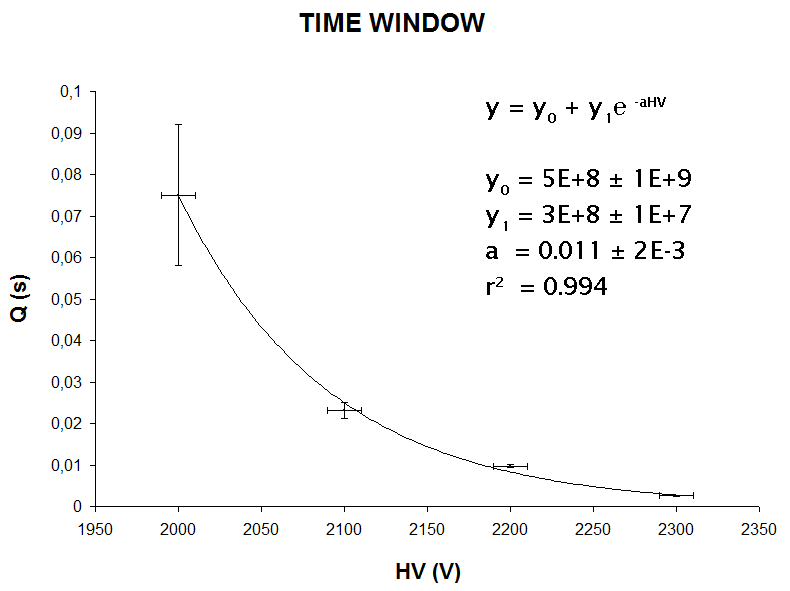
\includegraphics[width=\textwidth]{img/timeWindow.png}\ec
				\caption[Time window fit.]{Fit of the data points to an exponentially decreasing curve, whose fit parameters are shown with their error. The data is also represented with their error bars.}\label{fig:timeWin}
			\efi\vspace*{-1ex}

As discussed in Chapter \ref{chap:exp}, when the number of counts is large, ie, when the voltage is high, you should get a horizontal asymptote, whose value would be equivalent to the value of $Q$ at high number of counts. That is, when the approximation that $Q$ is of the order of the time window $\Delta T$ can be made.

The value is $\Delta T$ = 50 $\pm$ 1 ns, which agrees with $\Delta T \ll 0.15 s$. If our measuring system was very bad, a window of about $\mu$s would still be enough.
	
\subsection{Estimation of spurious coincidences and determination of the plateau}

To determine the plateau, two sets of measurements are made, as explained in Chapter \ref{chap:exp}. One by varying the voltage supplied to the detectors and the other by varying their threshold voltage. The starting voltages in each case are:

		\noindent\begin{minipage}{0.5\textwidth} 
			\bc
				Measurements varying the voltage:\\
				V$_{threshold1}$ = $-$34 $\pm$ 1 mV.\\
				V$_{threshold2}$ = $-$37 $\pm$ 1 mV.
			\ec
		\end{minipage}
		\begin{minipage}{0.5\textwidth} 
			\bc
				Measurements varying the threshold:\\
				V$_1$ = 2200 $\pm$ 1 V.\\
				V$_2$ = 2200 $\pm$ 1 V.
			\ec
		\end{minipage}

It's better to plot the curve while measuring, so that it is possible to detect and correct problems on the spot, and act accordingly.

If we plot the data of these two tables, there are some differences. The first difference is that the number of coincidences is bigger in Fig.~\ref{fig:voltage} than in Fig.~\ref{fig:threshold}, and it extends over a wider range (0-9 counts/s approximately, compared to the range of ~ 2-7 counts/s). This is consistent with the average count rate of N~/~t = 6 counts/s calculated in Chapter \ref{chap:exp}.

The contribution of random coincidences is negligible, so they are considered to neither contribute nor affect the measurements. Looking at Tables \ref{tab:voltage} and \ref{tab:threshold}, the ratio between the values of N$_{12}$  and N$_\text{random}$  is $\sim$~0.002\%.

Since we are working with the minimum threshold in the first case and the maximum voltage in the latter, the contribution of noise in the number of counts of each detector, and the spurious contributions to the number of coincidence counts should be the maximum. If these contributions are negligible, the time window has been set correctly.\vspace*{-1.5ex}

	\ctable [
	cap	    = {Determination of the plateau as a function of voltage.},
 	caption = {DETERMINATION OF PLATEAU AS A FUNCTION OF VOLTAGE. Measured voltage (HV), number of counts of detector 1 (N$_1$ / t) and detector 2 (N$_2$ / t) and coincidences (N$_{12}$ / t). From these data, the number of random coincidences N$_\text{random}$ has been calculated according to equation \ref{eq:random}. Errors and decimals presentsed are calculated as shown in Appendix \ref{chap:app3}.},
 	label   = {tab:voltage},
 	pos	    = H,
	botcap
	]
	{c c c c c}
	{}
 	{\FL
		\textbf{HV (V)} &
		\textbf{\pbox{.2\textwidth}{\pcen N$_1$ / t\\(counts/s)\\[1ex]}} &
		\textbf{\pbox{.2\textwidth}{\pcen N$_2$ / t\\(counts/s)\\[1ex]}} &
		\textbf{\pbox{.2\textwidth}{\pcen N$_{12}$ / t\\(counts/s)\\[1ex] 	}} &
		\textbf{\pbox{.2\textwidth}{\pcen N$_\text{random}$ / t\\(counts/s)\\[1ex]}} \\
		1600 $\pm$  1 & 103.7 $\pm$ 0.6 & 0.50  $\pm$ 0.04 & 0.18 $\pm$ 0.02 & 5.2E$-$6  $\pm$ 8E$-$7 \\
		1700 $\pm$  1 &  96.3 $\pm$ 0.6 & 3.0   $\pm$ 0.1  & 1.09 $\pm$ 0.06 & 2.9E$-$5  $\pm$ 2E$-$6 \\
		1800 $\pm$  1 &  92.0 $\pm$ 0.6 & 12.3  $\pm$ 0.2  & 2.8  $\pm$ 0.1  & 1.13E$-$4 $\pm$ 4E$-$6 \\
		1903 $\pm$  1 & 138.0 $\pm$ 0.7 & 249.3 $\pm$ 0.9  & 4.6  $\pm$ 0.1  & 3.4E$-$3  $\pm$ 1E$-$4 \\
		2000 $\pm$ 10 & 126.3 $\pm$ 0.6 & 143.7 $\pm$ 0.7  & 4.1  $\pm$ 0.1  & 1.81E$-$3 $\pm$ 5E$-$5 \\
		2100 $\pm$ 10 & 117.3 $\pm$ 0.6 & 347   $\pm$   1  & 4.8  $\pm$ 0.1  & 0.0041   $\pm$ 1E$-$4 \\
		2200 $\pm$ 10 & 110.0 $\pm$ 0.6 & 501   $\pm$   1  & 5.7  $\pm$ 0.1  & 0.0055   $\pm$ 1E$-$4 \\
		2300 $\pm$ 10 & 101.7 $\pm$ 0.6 & 1535  $\pm$   2  & 8.8  $\pm$ 0.2  & 0.0156   $\pm$ 1E$-$4
	\LL}\vspace*{-1.5ex}

	\ctable [
	cap	    = {Determination of the plateau as a function of the threshold.},
 	caption = {DETERMINATION OF PLATEAU AS A FUNCTION OF THRESHOLD. Measured threshold (V$_\text{threshold}$), number of counts of detector 1 (N$_1$ / t) and detector 2 (N$_2$ / t) and coincidences (N$_{12}$ / t). From these data, the number of random coincidences N$_\text{random}$ has been calculated according to equation \ref{eq:random}. Errors and decimals presented are calculated as shown in Appendix \ref{chap:app3}.},
 	label   = {tab:threshold},
 	pos	    = H,
	botcap
	]
	{c c c c c}
	{}
 	{\FL
		\textbf{\pbox{.2\textwidth}{\pcen V$_\text{threshold}$\\(mV)\\[1ex]}} &
		\textbf{\pbox{.2\textwidth}{\pcen N$_1$ / t\\(counts/s)\\[1ex]}} &
		\textbf{\pbox{.2\textwidth}{\pcen N$_2$ / t\\(counts/s)\\[1ex]}} &
		\textbf{\pbox{.2\textwidth}{\pcen N$_{12}$ / t\\(counts/s)\\[1ex]}} &
		\textbf{\pbox{.2\textwidth}{\pcen N$_\text{random}$ / t\\(counts/s)\\[1ex]}} \\
		$-$399   $\pm$ 1  & 14.7  $\pm$ 0.2 & 43.3 $\pm$ 0.4 & 2.8 $\pm$ 0.1 & 6.4E$-$5  $\pm$ 2E$-$6 \\ 
		$-$353   $\pm$ 1  & 17.7  $\pm$ 0.2 & 41.3 $\pm$ 0.4 & 2.9 $\pm$ 0.1 & 7.3E$-$5  $\pm$ 3E$-$6 \\
		$-$307   $\pm$ 1  & 21.3  $\pm$ 0.3 & 40.3 $\pm$ 0.4 & 2.8 $\pm$ 0.1 & 8.6E$-$5  $\pm$ 3E$-$6 \\ 
		$-$267   $\pm$ 1  & 25.3  $\pm$ 0.3 & 40.3 $\pm$ 0.4 & 2.7 $\pm$ 0.1 & 1.02E$-$4 $\pm$ 4E$-$6 \\
		$-$215   $\pm$ 1  & 33.3  $\pm$ 0.3 & 41.7 $\pm$ 0.4 & 3.0 $\pm$ 0.1 & 1.39E$-$4 $\pm$ 5E$-$6 \\
		$-$164   $\pm$ 1  & 51.0  $\pm$ 0.4 & 41.7 $\pm$ 0.4 & 3.0 $\pm$ 0.1 & 2.13E$-$4 $\pm$ 7E$-$6 \\
		$-$115   $\pm$ 1  & 247.0 $\pm$ 0.9 & 42.0 $\pm$ 0.4 & 3.6 $\pm$ 0.1 & 1.04E$-$3 $\pm$ 3E$-$5 \\
		$-$70.1 $\pm$ 0.1 & 1252  $\pm$ 2   & 41.3 $\pm$ 0.4 & 4.9 $\pm$ 0.1 & 0.0052   $\pm$ 1E$-$4 \\
		$-$35.2 $\pm$ 0.1 & 2492  $\pm$ 3   & 40.7 $\pm$ 0.4 & 6.3 $\pm$ 0.1 & 0.0101   $\pm$ 3E$-$4
	\LL}

			\bfi[H]
				\bc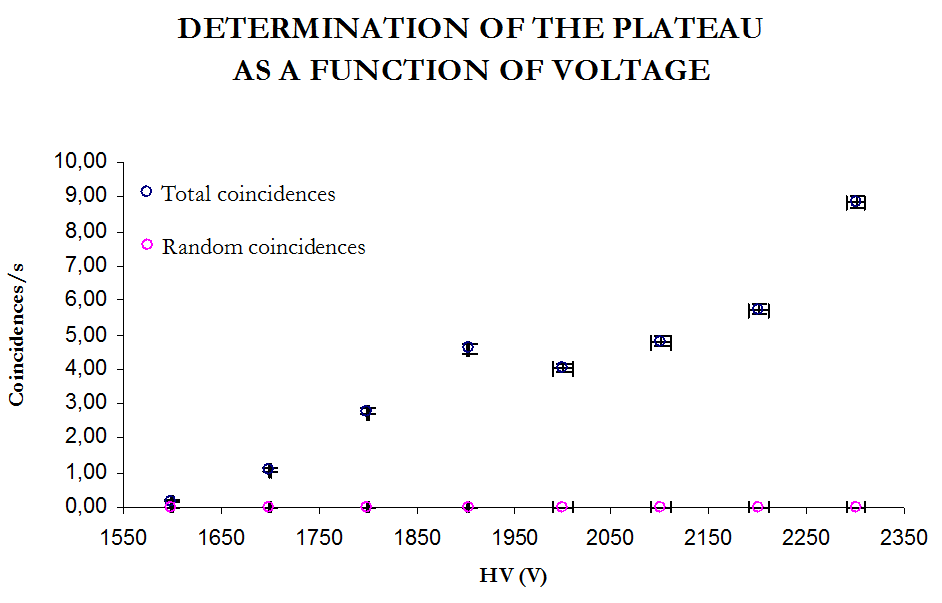
\includegraphics[width=\textwidth]{img/plateau1.png}\ec
				\caption[Coincidences against voltage.]{Coincidences against voltage.}\label{fig:voltage}
			\efi

			\bfi[H]
				\bc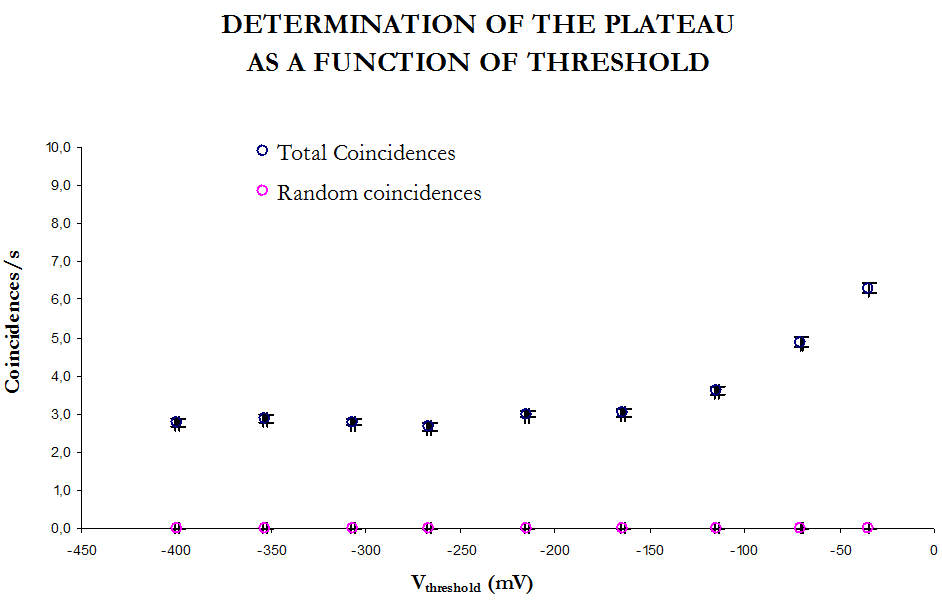
\includegraphics[width=\textwidth]{img/plateau2.png}\ec
				\caption[Coincidences against threshold.]{Coincidences against threshold.}\label{fig:threshold}
			\efi

Both the optimal working voltage and threshold for these detectors are roughly estimated from the data. They are taken from the most central part of the plateau, to avoid the areas of instability. The values are around:

	\graybox{.4}{.35}{\bc
		\noindent HV = 1900 $\pm$ 1 V \\
		\noindent V$_\text{threshold}$ = $-$200 $\pm$ 1 mV
	\ec}


The operating voltage set by the manufacturer for these scintilators can be around 2200 V, but the sensors age with use, which lowers the value of the working voltage over the years.



\section{Statistical characterization of cosmic radiation}

We can use different criteria to give the measure error $\epsilon$ in terms of percentages of the true value being in the range [$\mu - \epsilon$, $\mu + \epsilon$]. For example, according to the Gaussian distribution that represents the results, a new measure would likely fall in the range [$\mu - \sigma$, $\mu + \sigma$] with a probability of 0.683 (Appendix \ref{sec:gauss}). For this reason, $\sigma$ is also called the \textit{error of a single measurement}.


	\bi
		\item In the measurements taken at intervals of 5s, if you have a single measurement of $n$ counts, the best estimate of the true mean is this number $n$, and hence its standard deviation is $\sqrt n$ following the Poisson distribution. The data is given in the form: $n \pm \sqrt n$.

		\item From the results of the measurements every coincidences, we want to estimate their value and error under the hypothesis that, by grouping them in sets of increasing time, the values of these measures are distributed according to a  Gaussian distribution of mean $\mu$ and variance $\sigma^2$. Then we can determine that the best estimate of the mean of the distribution is the mean of the sample, $\bar{x}$. If several measurements are taken, the data is also given in the form: $\mu \pm \sqrt \mu$, with $\mu$ being the mean value.
	\ei

The values of the working voltages and thresholds for both detectors are set to the values obtained in the previous section. An example of the frequencies of the counts obtained at intervals of 5, 10 and 20s for 1 hour are shown below:

Fig.~\ref{fig:comparison} shows how as the collection time increases, the distribution is becoming increasingly flatter and wider and the maximum is shifting to the right.

Now it is time to calculate for each case the Poisson and Gaussian distributions. To compare with experimental data, we must first normalize them by dividing by the number of events $N$ that corresponds in each case.\vfill

	\ctable [
	cap	    = {Comparison of the number of coincidences.},
 	caption = {Comparison of the frequency of the number of coincidences for the measurements at intervals of 5, 10 and 20s.},
 	label   = {tab:comparison},
 	pos	    = H,
	botcap
	]
	{c c c c}
	{}
 	{\FL
		\textbf{Bin} &
		\textbf{5s} &
		\textbf{10s} &
		\textbf{20s}\\
		0 & 125 & 3  & 0 \\
		1 & 230 & 46 & 1 \\
		2 & 221 & 77 & 6 \\
		3 & 119 & 78 & 7 \\
		4 & 52  & 71 & 20 \\
		5 & 22  & 59 & 22 \\
		6 & 5   & 24 & 31 \\
		7 & 2   & 18 & 22 \\
		8 & 1   & 4  & 24 \\
		9 &     & 6  & 24 \\
		10 &    & 3  & 18 \\
		11 &    &    & 5 \\
		12 &    &    & 9 \\
		13 &    &    & 3 \\
		14 &    &    & 0 \\
		15 &    &    & 3
	\ML
		\textbf{AVERAGE}      & 1.8 & 3.6 & 7.2 \\
		\textbf{Standar Dev.} & 1.4 & 1.9 & 2.8 \\
		\textbf{N}            & 777 & 389 & 195
	\LL}\vspace*{-1ex}

	\bfi[H]
		\bc
			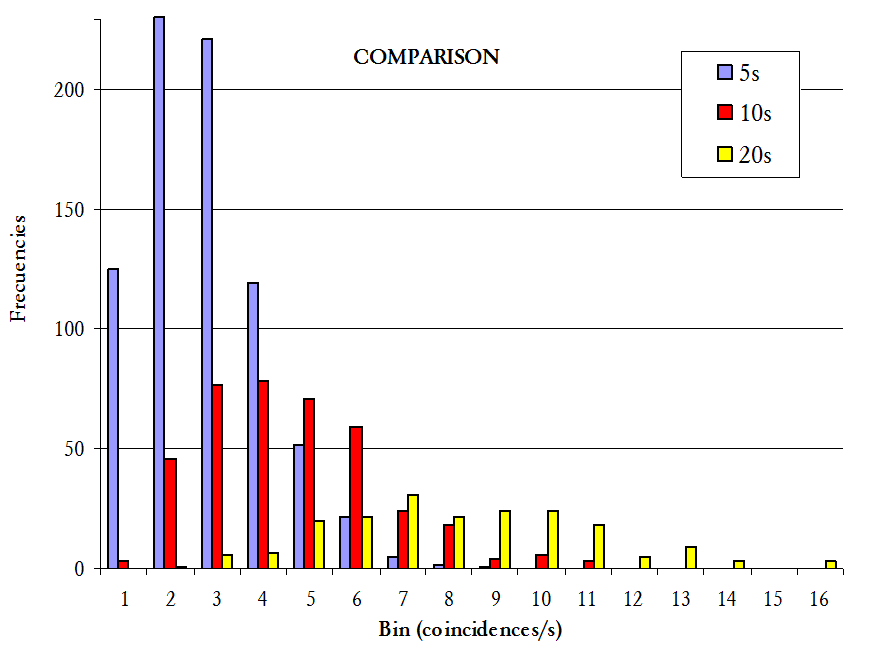
\includegraphics[width=.65\textwidth]{img/comparison.png}
			\caption
				[Frequency diagram.]
				{Frequency diagram for the number of coincidences every 5, 10, and 20s.}\label{fig:comparison}
		\ec
	\efi

\subsection{Measurements every 5s}

The table below shows that the Poisson expected values fit quite well to the experimental data within the error. However the expected values according to Gauss are a bit far from the experimental values, as expected.

	\ctable [
	cap	    = {Measurements every 5s.},
 	caption = {Measurements every 5s: Frequency of the number of coincidences and their expected value calculated using the Poisson and Gauss distributions.},
 	label   = {tab:5s},
 	pos	    = H,
	botcap
	]
	{c c c c}
	{}
 	{\FL
		\textbf{Bin} &
		\textbf{Exp.} &
		\textbf{Poisson} &
		\textbf{Gauss}\\
		0 & 0.16088 & 0.16521 & 0.12085 \\
		1 & 0.29601 & 0.29747 & 0.24884 \\
		2 & 0.28443 & 0.26780 & 0.29404 \\
		3 & 0.15315 & 0.16073 & 0.19939 \\
		4 & 0.06692 & 0.07235 & 0.07758 \\
		5 & 0.02831 & 0.02605 & 0.01732 \\
		6 & 0.00644 & 0.00782 & 0.00222 \\
		7 & 0.00257 & 0.00201 & 0.00016 \\
		8 & 0.00129 & 0.00045 & 0.00001
	\LL} 

	\bfi[H]
		\bc
			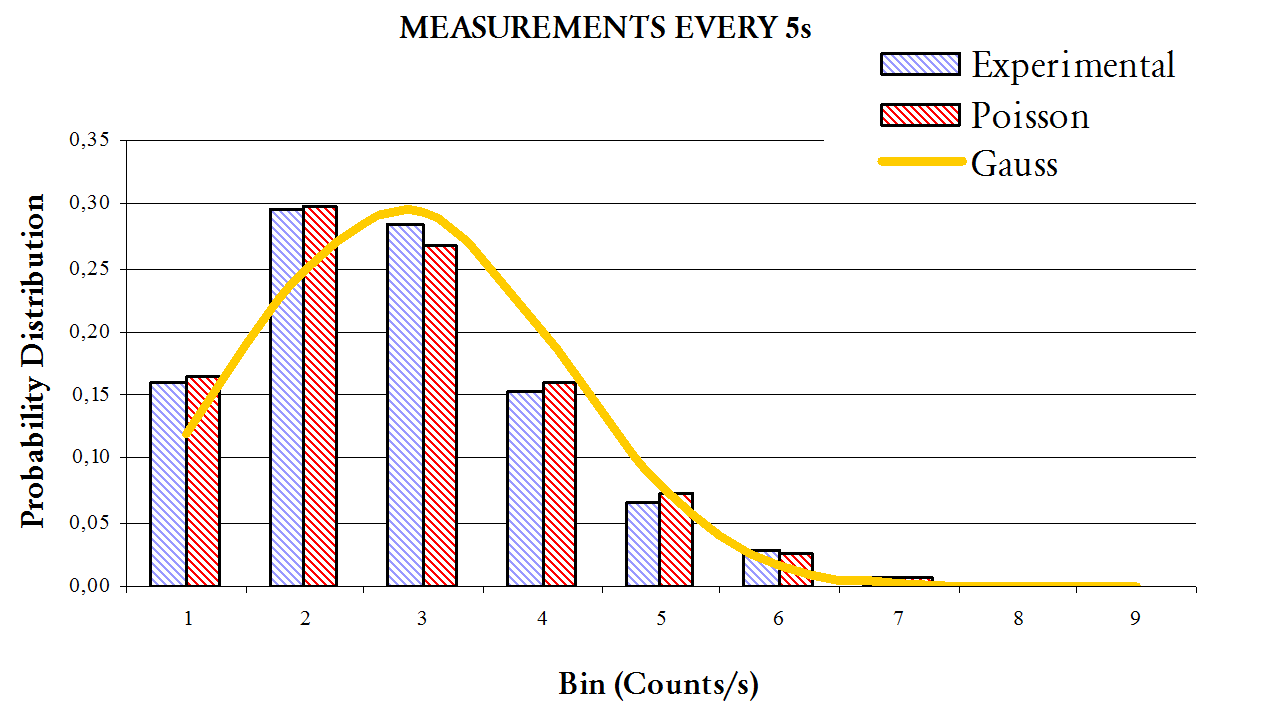
\includegraphics[width=.9\textwidth]{img/pdist1.png}
			\caption
				[Histogram for the measurements every 5s.]
				{Histogram of the number of coincidences each 5s compared to the expected value calculated using the Poisson and Gaussian distributions.}\label{fig:5s}
		\ec
	\efi

We have here a clear Poissonian curve with its maximum near the origin, as corresponds to the first part of the curve, which has a behavior proportional to $\mu^x$, while the right part of the maximum shows the typical Poisson decay, heavily dependent on the exponential decay of the $e^\mu$ distribution (Fig.~\ref{fig:5s}). 

This is corroborated by the theoretical values of the Poisson distribution, which fit very well to the data, as opposite to the Gauss distribution. The Poisson distribution is discrete so it is represented with bars, while the Gaussian is continuous so it represented with a line.

\subsection{Measurements every 10s}

If we take measurements every 10s, the data starts looking more like a Gauss distribution, although there is still no significant agreement. However, we see that the Poisson values have departed slightly from the experimental data compared with the previous table, and approaches the values as Gauss faster than experimental. This is best seen in the graphic.



We start to move away from the previous behavior, the Poissonian has shifted slightly to the right and has been flattened, seeking the Gaussian trend. Meanwhile the experimental data begins to look more like the Gaussian distribution.

	\ctable [
	cap	    = {Measurements every 10s.},
 	caption = {Measurements every 10s: Frequency of the number of coincidences and their expected value calculated using the Poisson and Gauss distributions.},
 	label   = {tab:10s},
 	pos	    = H,
	botcap
	]
	{c c c c}
	{}
 	{\FL
		\textbf{Bin} &
		\textbf{Exp.} &
		\textbf{Poisson} &
		\textbf{Gauss}\\
		0  & 0.0077 & 0.0274 & 0.0348 \\
		1  & 0.1183 & 0.0986 & 0.0824 \\
		2  & 0.1979 & 0.1773 & 0.1476 \\
		3  & 0.2005 & 0.2126 & 0.2002 \\
		4  & 0.1825 & 0.1911 & 0.2057 \\
		5  & 0.1517 & 0.1375 & 0.1600 \\
		6  & 0.0617 & 0.0824 & 0.0942 \\
		7  & 0.0463 & 0.0423 & 0.0420 \\
		8  & 0.0103 & 0.0190 & 0.0142 \\
		9  & 0.0154 & 0.0076 & 0.0036 \\
		10 & 0.0077 & 0.0027 & 0.0007
	\LL}


	\bfi[H]
		\bc
			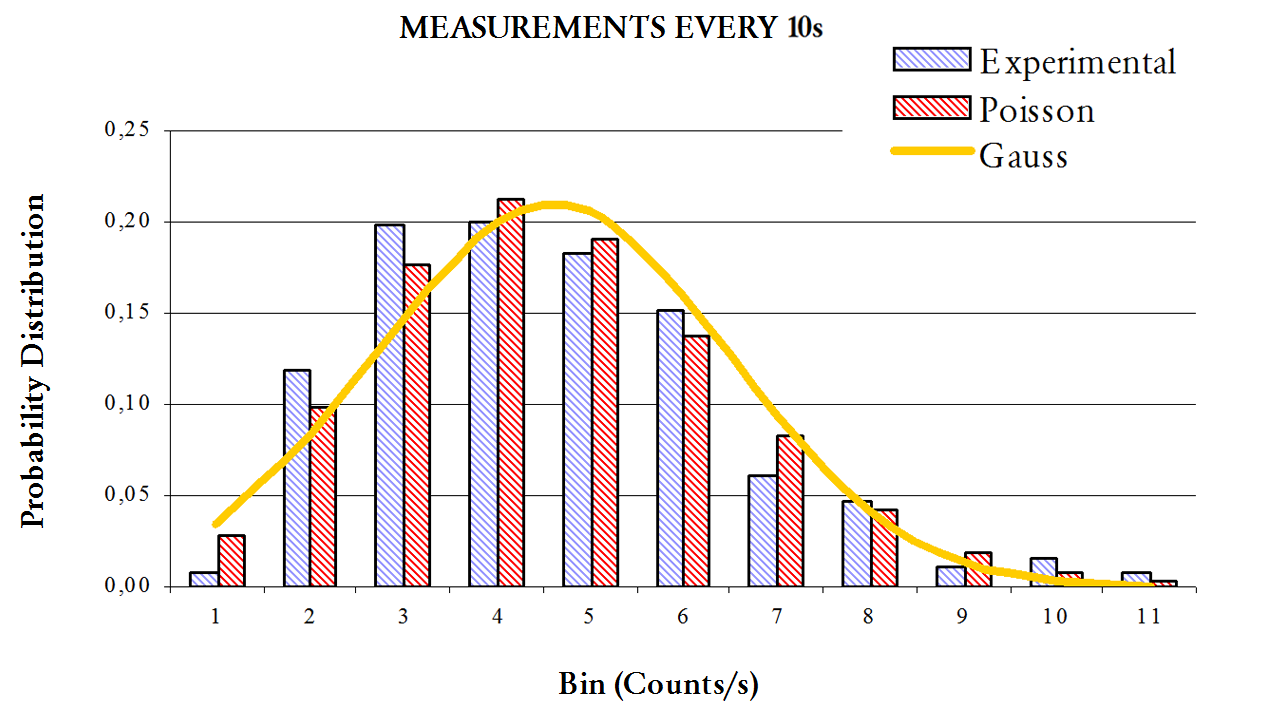
\includegraphics[width=.9\textwidth]{img/pdist2.png}
			\caption
				[Histogram for the measurements every 10s.]
				{Histogram of the number of coincidences grouped in intervals of 10s compared to the expected value calculated using the Poisson and Gaussian distributions.}\label{fig:10s}
		\ec
	\efi

\subsection{Measurements every 20s}

In this case, the Gauss distribution is even more similar to the experimental data, while Poisson continues to move away from their initial values. This will become evident in the graph below.

The data is nearly Gaussian, the Poissonian has abandoned its asymmetrical shape to become increasingly symmetrical, the peak has shifted to the right in search of the Gaussian and has flattened a little. With the increase of the measurement interval, the Poisson distributions gets closer to a Gaussian shape.

The experimental data also agree quite well with the Gaussian, removing some fluctuations like the maximum in bin 7 which is nothing more than a reminder of their old Poissonian tendency.

The shift of the Poisson distribution into a Gaussian is quite fast: with a difference of 5 or 10s in the measurement range, a fairly sharp change is seen in the shape of the distribution. This is remarkable because this distribution is modulated by only one parameter. The average $\mu$ alone makes the curve to flatter, moves its maximum and changes its width.

	\ctable [
	cap	    = {Measurements every 20s.},
 	caption = {Measurements every 20s: Frequency of the number of coincidences and their expected value calculated using the Poisson and Gauss distributions.},
 	label   = {tab:20s},
 	pos	    = H,
	botcap
	]
	{c c c c}
	{}
 	{\FL
		\textbf{Bin} &
		\textbf{Exp.} &
		\textbf{Poisson} &
		\textbf{Gauss}\\
		0  & 0     & 0.001 & 0.004 \\
		1  & 0.005 & 0.005 & 0.010 \\
		2  & 0.031 & 0.020 & 0.023 \\
		3  & 0.036 & 0.047 & 0.044 \\
		4  & 0.103 & 0.085 & 0.074 \\
		5  & 0.113 & 0.121 & 0.107 \\
		6  & 0.159 & 0.145 & 0.135 \\
		7  & 0.113 & 0.149 & 0.149 \\
		8  & 0.123 & 0.133 & 0.142 \\
		9  & 0.123 & 0.106 & 0.118 \\
		10 & 0.092 & 0.076 & 0.085 \\
		11 & 0.026 & 0.050 & 0.054 \\
		12 & 0.046 & 0.030 & 0.029 \\
		13 & 0.015 & 0.016 & 0.014 \\
		14 & 0     & 0.008 & 0.006 \\
		15 & 0.015 & 0.004 & 0.002
	\LL} 

	\bfi[H]
		\bc
			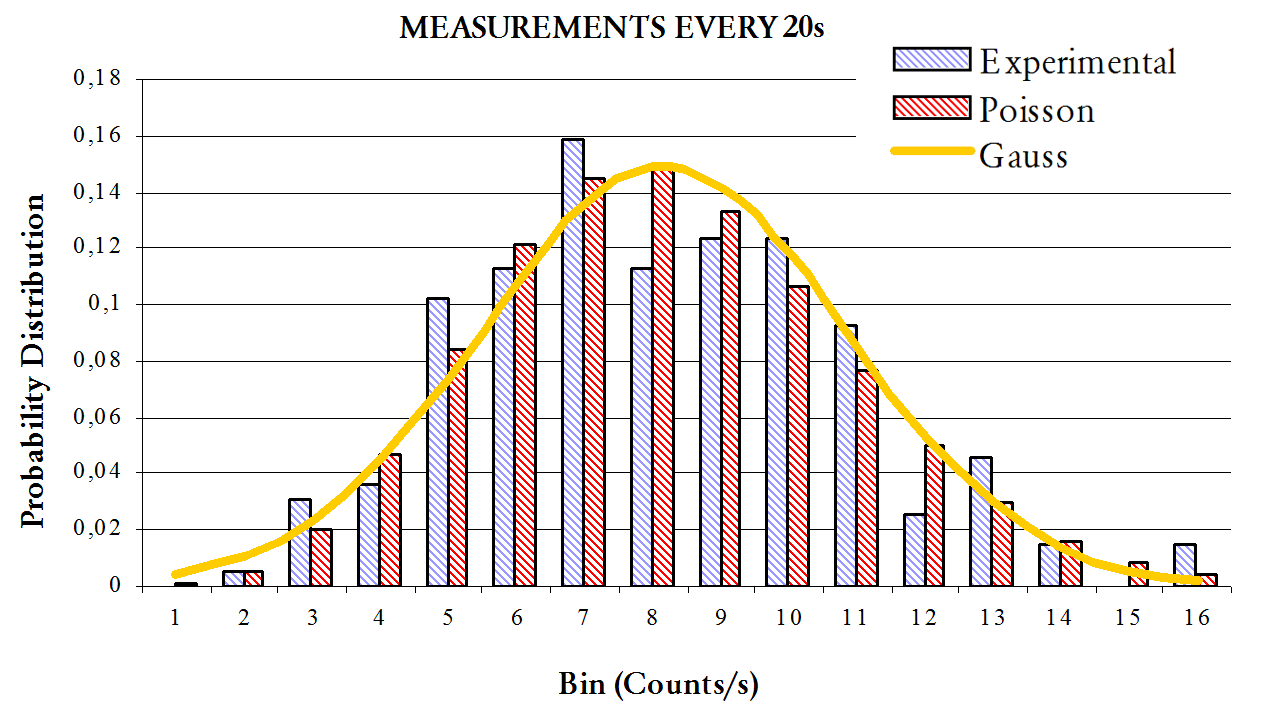
\includegraphics[width=.9\textwidth]{img/pdist3.png}
			\caption
				[Histogram for the measurements every 20s.]
				{Histogram of the number of coincidences grouped in intervals of 20s together with the expected values (solid lines) calculated according to the Poisson and Gauss distributions.}\label{fig:20s}
		\ec
	\efi

\subsection{Chi-square test results}

Given that the possible values of $\chi^2$ are distributed according to the Chi-squared distribution, whose expected value is equal to the number of degrees of freedom $\nu$, which in turn is equal to the number of experimental points $n$ (which is the number of corresponding frequencies in each case), minus the number of parameters or constraints $k$, which in this case is found to be 2, the mean $\mu$ and the number of data $N$, and whose standard deviation is $\sigma = \sqrt{2\nu}$
(Appendix \ref{sec:chi2}) it is possible to establish a measure of the quality of fit (Table \ref{tab:chieval}):


	\ben
		\item If the fit provides a $\chi^2$ that is less than 3$\sigma$ of its expected value, we can speak of an acceptable fit.

		\item If the $\chi^2$ value is much less of its expected value, presumably the assigned errors $\sigma_i$ have been overestimated. In this case, the experiment must be repeated.

		\item If the $\chi^2$ is at more than 3$\sigma$ from its expected value, several problems may be the cause:
			\bi 
				\item The set of measurements is incorrect.
				\item The assigned errors are too small.
				\item The model function is inadequate.
			\ei
	\een

As a general rule, it is assumed that being $\chi_\text{exp}^2$ the value found for $\chi^2$, if

	\bc $P \left(\chi^2 < \chi_\text{exp}^2\right) = \sum_{-\infty}^{\chi_c^2} P_\nu(x) \,dx$\ec

is between 0.1 and 0.9, the hypothesis is correct, given that this judgment has a confidence level equal to CL = $P \left(\chi^2 < \chi_\text{exp}^2\right) \times$ 100\% (Appendix \ref{sec:chi2}).

For a total of 8 frequencies in the first case (5s), 10 frequencies in the second (10s) and 15 in the third (20s), and having two constraints in all cases, since the Gaussian limit of the Poisson distribution still has one parameter (the mean $\mu$), values of 6, 8 and 13 are obtained respectively for $\nu$. The confidence intervals between which $\chi^2 = \chi_\text{exp}^2$ is situated can be calculated for the different degrees of freedom according to Table \ref{tab:chieval}:

	\ctable [
	cap	    = {Intervals between which $\chi_c^2$ is located.},
 	caption = {Intervals between which $\chi_c^2$ is located according to the different degrees of freedom obtained in this section. P values are taken from Table \ref{tab:chieval}.},
 	label   = {tab:intervals},
 	pos	    = H,
	botcap
	]
	{c c c c c}
	{}
 	{\FL
		\textbf{$\chi_c^2$} &
		\textbf{$\nu$ = 6}  &
		\textbf{$\nu$ = 8}  &
		\textbf{$\nu$ = 13} &
		\textbf{$P \left(\chi^2 < \chi_\text{exp}^2\right)$}\\[1ex]
		$\nu \pm 3\sigma$ & ($-$4.390 $< \chi_c^2 <$ 16.392) & ($-$4 $< \chi_c^2 <$ 20) & ($-$2.297 $< \chi_c^2 <$ 28.297) & 0.99\\[1.5ex]
		$\nu \pm 2\sigma$ & ($-$0.900 $< \chi_c^2 <$ 12.928) & (0 $< \chi_c^2 <$ 16)  & (2.802 $< \chi_c^2 <$ 23.198)  & 0.96\\[1.5ex]
		$\nu \pm \sigma$  & (2.536 $< \chi_c^2 <$ 9.464)   & (4 $< \chi_c^2 <$ 12)  & (7.901 $< \chi_c^2 <$ 18.099)  & 0.85\\[1.5ex]
		$\nu$             & $\chi_c^2$ = 6                 & $\chi_c^2$  = 8        & $\chi_c^2$  = 13               & 0.55
	\LL} 

Since this table is very limited because it shows the value of $P$ for a whole interval, the exact value of the confidence level corresponding to each given value of $\chi_c^2$ obtained experimentally using the program at the end of Appendix \ref{chap:app4}. The $\chi_c^2$ obtained from the data in Tables \ref{tab:5s}-\ref{tab:20s} are shown below:

	\ctable [
	cap	    = {Values of time, degrees of freedom and $\chi^2$.},
 	caption = {Values of time, degrees of freedom and $\chi^2$ obtained for the Poisson distribution or P (x) and Gauss or G (x) with their confidence level calculated according the \code{cl.cpp} program.},
 	label   = {tab:clcpp},
 	pos	    = H,
	botcap
	]
	{c c c c c c}
	{}
 	{\FL
		\textbf{Time (s)} &
		\textbf{$\nu$}  &
		\textbf{\pbox{.1\textwidth}{\pcen$\chi_\text{exp}^2$ P(x)\\[1ex]}}  &
		\textbf{\pbox{.2\textwidth}{\pcen Confidence level according to \code{cl.cpp}\\[1ex]}} &
		\textbf{\pbox{.1\textwidth}{\pcen$\chi_\text{exp}^2$ G(x)}}  &
		\textbf{\pbox{.2\textwidth}{\pcen Confidence level according to \code{cl.cpp}\\[1ex]}} \\
		5  & 6  & 0.004 & 0.998002 & 0.323 & 0.850866 \\
		10 & 8  & 0.050 & 0.97531  & 0.178 & 0.914846 \\
		20 & 13 & 0.092 & 0.955042 & 0.153 & 0.926353
	\LL} 

With these values of $\chi^2$ and our number of constraints (2) we run the program \code{cl.cpp} (Appendix \ref{sec:chi2}) and obtain the confidence levels shown for each of the values of $\chi^2$.

There is certain compatibility observed between the values of \code{cl.cpp} and Table \ref{tab:intervals}, as in the case of $\nu$ = 6 for example, both the value of $\chi_\text{exp}^2 P(x)$ and $\chi_\text{exp}^2 G(x)$ are less than 3$\sigma$ of its expected value $\nu$, since they are in the range $\nu \pm 2\sigma$, so according to item 1 of this section, both fits would be good, but in the case of $P(x)$ the program gives a higher confidence value than for $G(x)$.

The value of $\chi^2$ grows for the Poisson distribution as we increase the measuring time, so the confidence level decreases from 99.8\% to 95.5\%. According to this, we would say with certainty that the experimental data fit a Poisson distribution in the measurements every 5s, with a confidence of 99.8\%.

Furthermore, the effect of grouping measurements in greater time intervals, makes the $\chi^2$ of the Gaussian distribution to decrease, so its confidence level increases from 85.1\% to 92.6\%, although without reaching the values of the Poissonian. Therefore, in the case of measurements of 20s, we could say that the data follows a Gaussian with a security of \enquote{only} the 92.6\%, which is not bad although our confidence is lower than in the case of Poisson at 5s.

It follows that, in the first case, we must reject the hypothesis of the Gaussian, in the second case is still Poissonian, and in the third case there is no reason to rule out the Gaussian assumption, as the confidence level, although lower, is high enough.


If coincidences were grouped into larger time intervals, of 40s or minutes, we would get increasingly higher values of $\chi^2$ for the Poisson distribution and lower for the Gaussian distribution, which would translate into a higher level of confidence for Gauss, confirming the hypothesis that \textbf{cosmic radiation has a Gaussian probability distribution}. In fact, some books \cite{kno:79} say that when the mean of a distribution (binomial at least) is greater than 30 events, the distribution is Gaussian.

And so the statistical nature of cosmic radiation is well demonstrated.



\section{Separation of the hard component of coincidences}


In this section it is important to wait longer (around an hour) for each measurement, in order to get a number of counts with an error of $\sim$5--10\%. The distance between scintillators is 30.0 $\pm$ 0.1 cm. The method of analysis discussed in section \ref{chap:exp} is broken down here briefly.

The fits obtained for Al and Pb must give compatible values for the value of the components at zero thickness. Typical experimental values for the attenuation in lead and aluminium are (errors and decimals presented are calculated according to Appendix~\ref{chap:app3}):

	\ctable [
	cap	    = {Attenuation in lead.},
 	caption = {Increasing thickness of the layers of Pb (an error of $\pm$ 1 mm has been considered) along with the number of coincidences ($N_{12}$ / t). Measurements with the lead blocks were also made, as well as mixing blocks and thin layers.},
 	label   = {tab:lead},
 	pos	    = H,
	botcap
	]
	{c c c}
	{}
 	{\FL
		\textbf{x (cm)} &
		\textbf{\pbox{.3\textwidth}{\pcen$N_{12}$ / t\\(coinc./s)\\[1ex]}}  &
		\textbf{\pbox{.3\textwidth}{\pcen Error / t\\(coinc./s)\\[1ex]}}  \\
		0    & 0.82 & 0.03 \\
		0.3  & 0.88 & 0.04 \\
		0.6  & 0.86 & 0.04 \\
		0.9  & 0.78 & 0.04 \\
		1.2  & 0.71 & 0.03 \\
		 5   & 0.62 & 0.03 \\
		10   & 0.63 & 0.03 \\
		15   & 0.56 & 0.03 \\
		20   & 0.53 & 0.03 \\
		20.9 & 0.55 & 0.03 \\
		21.2 & 0.55 & 0.03 \\
		21.5 & 0.55 & 0.03 \\
		25   & 0.51 & 0.03
	\LL}

	\ctable [
	cap	    = {Attenuation in aluminium.},
 	caption = {Increasing thickness of the layers of Al (an error of $\pm$ 1 mm has been considered) along with the number of coincidences ($N_{12}$ / t).},
 	label   = {tab:alum},
 	pos	    = H,
	botcap
	]
	{c c c}
	{}
 	{\FL
		\textbf{x (cm)} &
		\textbf{\pbox{.3\textwidth}{\pcen$N_{12}$ / t\\(coinc./s)\\[1ex]}}  &
		\textbf{\pbox{.3\textwidth}{\pcen Error / t\\(coinc./s)\\[1ex]}}  \\
		0  & 1.00 & 0.04 \\
		3  & 0.90 & 0.04 \\
		6  & 0.91 & 0.04 \\
		9  & 0.85 & 0.04 \\
		12 & 0.81 & 0.04 \\
		15 & 0.73 & 0.03 \\
		18 & 0.78 & 0.04 \\
		21 & 0.74 & 0.04 \\
		24 & 0.73 & 0.03 \\
		27 & 0.78 & 0.04
	\LL}


	\graybox{.9}{.75}{
		\bc\textcolor{gray}{\Large{\sffamily Exponential Fit:}}\ec

		Should conform to the function:

		\bc$f(x) = A_1e^{-\frac{x}{b_1}} + A_2e^{-\frac{x}{b_2}}$\ec

		where $b_i = \frac{\Lambda_i}{\rho_\text{Pb}}$, and the slower exponential decay corresponds to the hard component.\\

		Considering for example, the first exponential as the correspondent to the hard component, $A_1$ would be the amount of $\mu^\pm$ (the hard component) at zero thickness, and $A_2$ the amount of e$^\pm$ (the soft component) at zero thickness. The value of $f(x)$ at $x$ = 0 gives the sum of these two contributions.\\

		If the exponential part of the soft component falls much faster than the hard one, it means that $b_2$ is much smaller than $b_1$, and in the appropriate data range ($b_2 \ll x \ll b_1$) the second exponential tends to zero. Then, $f(x)$ behaves as a straight line intersecting the Y axis $A_1$:
		\bc$f(x) \sim A_1\left(1 - \frac{x}{b_1}\right) \qquad$ in $b_2 \ll x \ll b_1$\ec

		With the $b_1$ obtained from this fit, is easy to see that the experimental values of $x$ are in the proper range ($x_i \ll b_1$) and that this linear approximation is valid.
	}

\subsection{Fit for Lead}

For the \textbf{soft component} we obtain $b_1 = \mu_1^{-1} = \Lambda_1 / \rho_\text{Pb}$ = 4.7 $\pm$  0.3 cm (Fig. \ref{fig:lead}) so:\vspace{-1ex}
\bc $\mu_1$ = 0.213 $\pm$ 0.009 cm$^{-1} \qquad$ and $\qquad \Lambda_1$ = 5 $\pm$ 2 g cm$^{-2}$\ec


and taking the value of $A_1$ (the rate of soft component at zero thickness), if $S$ is the surface of the detectors, the flux of soft component is,

	\bfi[H]
		\begin{minipage}{.8\textwidth}
			\bc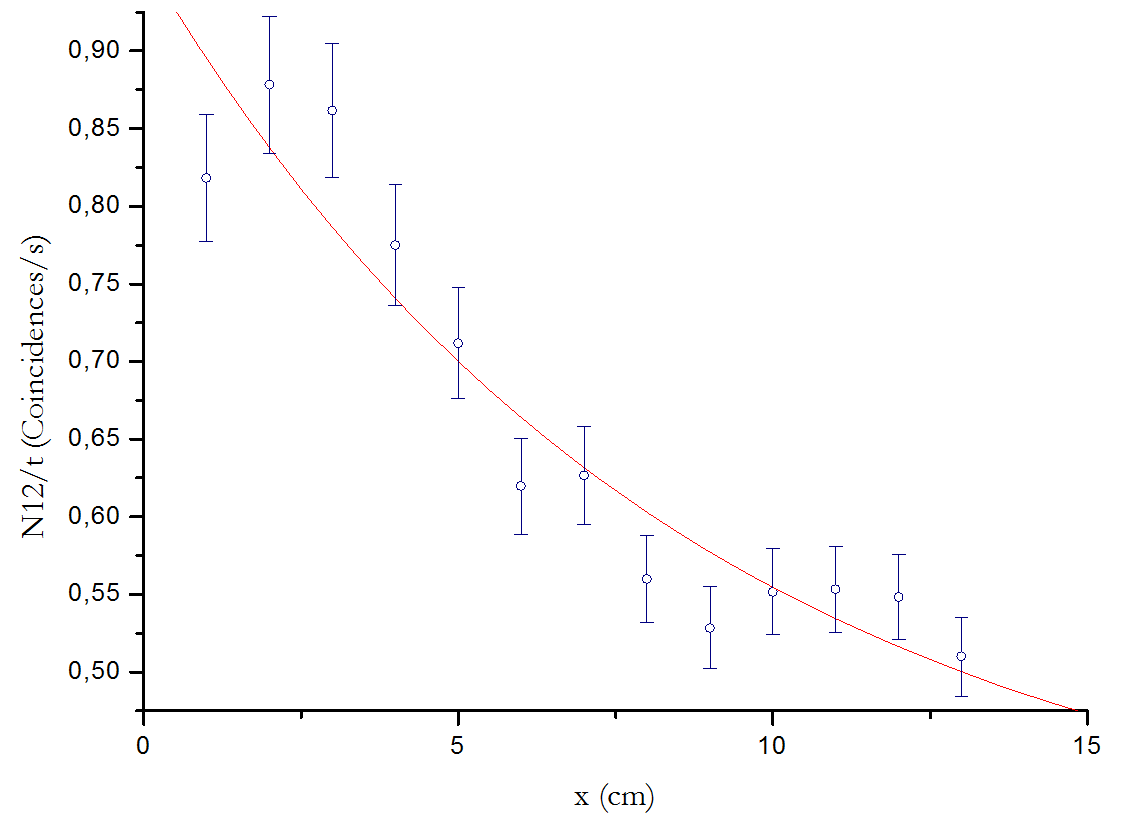
\includegraphics[width=\textwidth]{img/atenuationPb.png}\ec
		\end{minipage}\begin{minipage}{.2\textwidth}
			$\chi^2$ = 0.00248\\
			$r^2$ = 0.89735\\

			$A_1$ = 0.4 $\pm$ 0.2\\
			$b_1$ = 4.7 $\pm$ 0.3\\

			$A_2$ = 0.6 $\pm$ 0.1\\
			$b_2$ = 9 $\pm$ 5\\
		\end{minipage}
		\caption
			[Attenuation in lead.]
			{Attenuation of cosmic radiation passing through layers of lead, with error bars and fit results.}\label{fig:lead}
	\efi

\graybox{.4}{.35}{\bc $J_s = \frac{N_s/t}{S}$ = 13 $\pm$ 6 m$^{-2}$s$^{-1}$\ec}

The errors are calculated according to Appendix \ref{chap:app3}. The value of $J$ is a bit low compared to the theoretical value in Table \ref{tab:rppp}, this is due to the effect of the geometric efficiency, given that detectors have to be separated by a distance.

For the \textbf{hard component}, $b_2 = \mu_2^{-1} = \Lambda_2 / \rho_\text{Pb}$ = 9 $\pm$ 5 cm, which:

\bc $\mu_2$ = 0.11 $\pm$ 0.06 cm$^{-1} \qquad$ and $\qquad \Lambda_2$ = 102 $\pm$ 55 g cm$^{-2}$\ec

and the flux of the hard component is,

\graybox{.4}{.35}{\bc $J_h = \frac{N_h/t}{S}$ = 19 $\pm$ 3 m$^{-2}$s$^{-1}$\ec}

Its value is also far from the theoretical value shown in Table \ref{tab:rppp}, however, the linear absorption coefficient $\mu$ for muons is lower than for the soft component, as expected.

\graybox{.9}{.75}{
	As already mentioned, if the soft component falls much faster than the hard one, since $b_1$ would be much lower than $b_2$, in an appropriate data range $b_1 \ll x \ll b_2$, the first exponential tends to zero, and $f(x)$ behaves like a straight line intersecting the Y axis in $A_2$:
		\bc$f(x) \sim A_2\left(1 - \frac{x}{b_2}\right) \qquad$ in $b_1 \ll x \ll b_2$\ec
	In this part, error handling is not needed since a qualitative approach is enough, and we choose the range below and make a linear fit to it:\\

	\begin{minipage}{.3\textwidth}
		\begin{tabular}{ c c }
			\hline
  			\textbf{x (cm)} &
			\textbf{$N_{12}/t$} \\
			10 & 0.63 \\
			15 & 0.56 \\
			20 & 0.53 \\
			25 & 0.51 \\
			\hline
		\end{tabular}
	\end{minipage}\begin{minipage}{.7\textwidth}
		$y$ = 0.690 $\pm$ 0.008$x$\\
		$r^2$ = 0.923\\

		$A_2$ = 0.6898 s$^{-1}$\\
		$b_2$ = $A_2$/0.0076 = 90.76 cm$^{-1}$s$^{-1}$
	\end{minipage}\vspace*{2ex}

	With the value of $b_2$ obtained from this fit, we can check that the experimental values of $x$ are in the proper range ($x_i \ll b_2$) and that this linear approximation is valid. In this case the value of $b_2$ which is 10 times larger than the one obtained previously, but indeed in the range of $x$ chosen $x \ll b_2$ is fulfilled, so the linear approximation in that range is valid, and the value of $A_2$ (hard component at zero thickness) is compatible with the value obtained before.
}



\subsection{Fit for Aluminum}

	\bfi[H]
		\begin{minipage}{.78\textwidth}
			\bc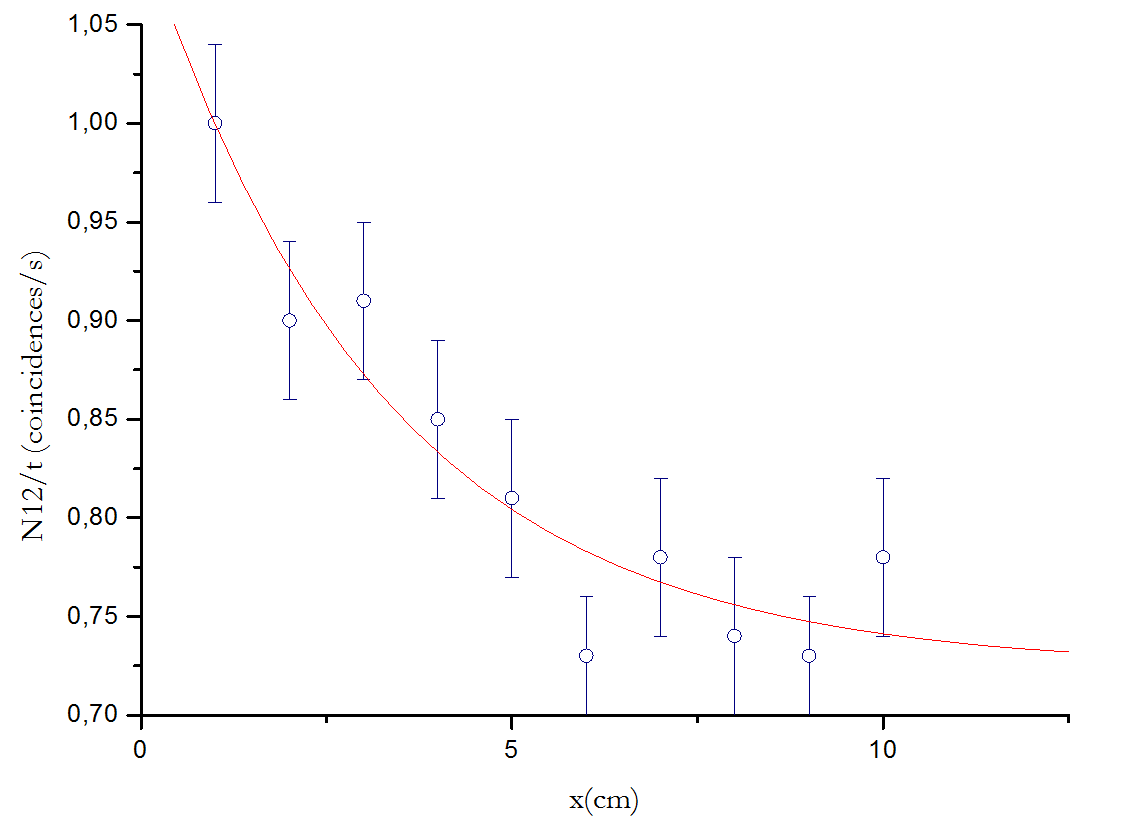
\includegraphics[width=\textwidth]{img/atenuationAl.png}\ec
		\end{minipage}\begin{minipage}{.22\textwidth}
			$\chi^2$ = 0.00124\\
			$r^2$ = 0.89909\\

			$A_1$ = 0.68 $\pm$ 0.04\\
			$b_1$ = 3.5 $\pm$ 0.4\\

			$A_2$ = 0.37 $\pm$ 0.06\\
			$b_2$ = 3 $\pm$ 1\\
		\end{minipage}
		\caption
			[Attenuation in lead.]
			{Attenuation of cosmic radiation passing through layers of aluminium, with the fit and error bars.}\label{fig:alum}
	\efi


For the \textbf{hard component}, $b_1 = \mu_1^{-1} = \Lambda_1 / \rho_\text{Al}$ = 3.5 $\pm$ 0.4 cm, so we get:

\bc $\mu_1$ = 0.29 $\pm$ 0.03 cm$^{-1} \qquad$ and $\qquad \Lambda_1$ = 9 $\pm$ 1 g cm$^{-2}$\ec

and the flux of the hard component is,

\graybox{.4}{.35}{\bc $J_h = \frac{N_h/t}{S}$ = 22 $\pm$ 1 m$^{-2}$s$^{-1}$\ec}

The errors were calculated according to Appendix \ref{chap:app3}. Again it is observed that the value remains low compared to the theoretical value in Table \ref{tab:rppp}, and for the same reason.

For the \textbf{soft component} we obtain $b_2 = \mu_2^{-1} = \Lambda_2 / \rho_\text{Pb}$ = 3 $\pm$ 1 cm so:

\bc $\mu_2$ = 0.3 $\pm$ 0.1 cm$^{-1} \qquad$ and $\qquad \Lambda_2$ = 8 $\pm$ 3 g cm$^{-2}$\ec

and the flux of soft component is,

\graybox{.4}{.35}{\bc $J_s = \frac{N_s/t}{S}$ = 12 $\pm$ 2 m$^{-2}$s$^{-1}$\ec}

Again, it is a bit low compared to the theoretical value in Table \ref{tab:rppp}, but the $\mu$ for muons is again smaller than for electrons.

The results can also be explained by the fact that the roof attenuates some part of the soft component, but not the hard one, so less soft component is measured compared to what would be obtained under different conditions.


\graybox{.9}{.75}{
	As before, if the soft component falls much faster than the hard one, since $b_2$ would be much lower than $b_1$, in an appropriate data range $b_2 \ll x \ll b_1$, the first exponential tends to zero, and $f(x)$ behaves like a straight line intersecting the Y axis in $A_1$:
		\bc$f(x) \sim A_1\left(1 - \frac{x}{b_1}\right) \qquad$ in $b_2 \ll x \ll b_1$\ec

	Linear fit to the data range on the left:\\

	\begin{minipage}{.3\textwidth}
		\begin{tabular}{ c c }
			\hline
  			\textbf{x (cm)} &
			\textbf{$N_{12}/t$} \\
			12 & 0.81 \\
			18 & 0.78 \\
			21 & 0.74 \\
			24 & 0.73 \\
			\hline
		\end{tabular}
	\end{minipage}\begin{minipage}{.7\textwidth}
		$y$ = 0.9019 $\pm$ 0.0074$x$\\
		$r^2$ = 0.9529\\

		$A_1$ = 0.9019 s$^{-1}$\\
		$b_1$ = $A_1$/0.0074 = 121.9 cm$^{-1}$s$^{-1}$
	\end{minipage}\vspace*{2ex}

	With the value of $b_1$ obtained from this fit, we can check that the experimental values of $x$ are in the proper range ($x_i \ll b_1$) and that this linear approximation is valid.\\
}
\graybox{.9}{.75}{
	In this case the value of $b_1$ which is 10 times larger than the one obtained previously, but indeed in the range of $x$ chosen $x \ll b_1$ is fulfilled, so the linear approximation in that range is valid, and the value of $A_1$ (hard component at zero thickness) is compatible with the value obtained before.
}

The number of particles of the soft and hard component obtained at zero thickness  for Al and Pb should be compatible, as shown in the table below.

	\ctable [
	cap	    = {Hard and soft components at zero thickness.},
 	caption = {Hard and soft components at zero thickness.},
 	label   = {tab:atzero},
 	pos	    = H,
	botcap
	]
	{l c c c}
	{}
 	{\FL
		&
		\textbf{Hard} &
		\textbf{Soft} &
		\textbf{Total} \\
		Lead      & 
		19 $\pm$ 3 m$^{-2}$s$^{-1}$ & 
		13 $\pm$ 6 m$^{-2}$s$^{-1}$ &
		32 $\pm$ 9 m$^{-2}$s$^{-1}$ \\
		Aluminium &
		22 $\pm$ 1 m$^{-2}$s$^{-1}$ &
		12 $\pm$ 2 m$^{-2}$s$^{-1}$ &
		34 $\pm$ 3 m$^{-2}$s$^{-1}$
	\LL}

Remember that these data have to be taken at $d$ = 30 cm. and thickness $x$ = 0 cm. In the case of the hard component, there is a bit larger difference between the two results at zero thickness, but this difference is at the limit of error, while for the soft component there is a great agreement.


\section{Calculation of the geometric efficiency}

Taking the data obtained in the previous section for the hard and soft components (with detectors at $d$ = 30.0 $\pm$ 0.1 cm), and the first experimental data we obtained in this section for $d$ = 0 cm. The following table is obtained:

	\ctable [
	cap	    = {Summary of experimental data obtained for $J$ in the previous section.},
 	caption = {Summary of experimental data obtained for $J$ in the previous section contrasted with theory and with data for $d$ = 0.},
 	label   = {tab:summary},
 	pos	    = H,
	botcap
	]
	{l c c c c}
	{}
 	{\FL
		&
		\multicolumn{2}{c}{\textbf{Hard (m$^{-2}$s$^{-1}$)}} &
		\multicolumn{2}{c}{\textbf{Soft (m$^{-2}$s$^{-1}$)}} \\
		\cmidrule(rl){2-3}\cmidrule(l){4-5}
		Theory      & 
		\multicolumn{2}{c}{130} &
		\multicolumn{2}{c}{ 50} \\
		\cmidrule(r){1-1}\cmidrule(rl){2-3}\cmidrule(l){4-5}
		\multirow{2}{.2\textwidth}{Experiment at $d$ = 30 cm and thickness $x$ = 0} &
		Lead & Aluminum & Lead & Aluminum \\ 
		& 19 $\pm$ 3 & 22 $\pm$ 1 & 13 $\pm$ 6 & 12 $\pm$ 2 \\
		& & & & \\
		\cmidrule(r){1-1}\cmidrule(l){2-5}
		\pbox{.2\textwidth}{\pcen Experiment at $d$ = 0 cm\\[1ex]} &
		\multicolumn{4}{c}{34.2 $\pm$ 0.6 (Total flux)} 
	\LL}


There is a growth in the number of total particles that are detected with the scintillators attached. In this section, one of the possible causes of the inconsistency between theory and experiment mentioned in the previous section will be addressed.

\subsection{Experimental measurements}

For each value of the distance between scintillators, six measurements of the coincidences are taken, in order to calculate the average, thus the error is given by the dispersion $\sigma$ (Appendix \ref{chap:app3}). The duration of each measurement is six minutes. The working conditions are set to these values:

\bc
HV$_1$ = 1900 V, V$_\text{threshold}$ = $-$200 mV\\
HV$_2$ = 1900 V, V$_\text{threshold}$ = $-$200 mV\ec

The data in Table \ref{tab:avcoinc} is obtained.

	\ctable [
	cap	    = {Coincidences as a function of distance.},
 	caption = {Increasing values of $d$ (an error of $\pm$ 1 mm has been considered) along with the number of averaged coincidences (N$_{12}$ av./t). It also presents the ratio N$_{12}$(d) /N$_{12}$(0) , where N$_{12}$(d) is the number of coincidences with the detectors at a distance d, and N$_{12}$(0) the number of coincidences when the detectors are together. Errors and decimals presented are calculated as shown in Appendix \ref{chap:app3}.},
 	label   = {tab:avcoinc},
 	pos	    = H,
	botcap
	]
	{c c c}
	{}
 	{\FL
		\textbf{d (cm)} &
		\textbf{\pbox{.3\textwidth}{\pcen N$_{12}$ av./t\\(counts / s)\\[1ex]}} &
		\textbf{\pbox{.3\textwidth}{\pcen N$_{12}$(d) /N$_{12}$(0) \\(counts / s)\\[1ex]}}\\
		0.0  & 1.06  $\pm$ 0.02 & 1.00   $\pm$ 0.03 \\
		5.5  & 0.46  $\pm$ 0.01 & 0.43   $\pm$ 0.02 \\
		8.5  & 0.29  $\pm$ 0.01 & 0.27   $\pm$ 0.01 \\
		11.0 & 0.21  $\pm$ 0.01 & 0.20   $\pm$ 0.01 \\
		15.5 & 0.158 $\pm$ 0.008 & 0.149 $\pm$ 0.008 \\
		19.5 & 0.100 $\pm$ 0.006 & 0.094 $\pm$ 0.006 \\
		23.5 & 0.092 $\pm$ 0.006 & 0.086 $\pm$ 0.006 \\
		25.0 & 0.069 $\pm$ 0.006 & 0.065 $\pm$ 0.005
	\LL}

In this case the ratio of N$_{12}$(d) and N$_{12}$(0) is the geometric efficiency  calculated from experimental data for each distance, as explained in chapter \ref{chap:exp}. We see that as the distance between scintillators increases, the efficiency decreases by 94\% from 1 for the most ideal case (with the scintillators at $d$ = 0), to 0.06 for a distance of 25 cm. Even when separated 5 cm we have a loss of just over 50\%.

\subsection{Monte-Carlo simulation (Appendix \ref{chap:app2})}

Simulate a flux of 10000 particles for the same distances used in the experimental measurements.  You should obtain something as the data in Table \ref{tab:geff}.

	\ctable [
	cap	    = {Geometric efficiency.},
 	caption = {Increasing values of d (with an error of $\pm$ 1 mm) with the number of counts that fell within the detector (n). The geometric efficiency is also presented. Calculation errors are not considered in these data.},
 	label   = {tab:geff},
 	pos	    = H,
	botcap
	]
	{c c c}
	{}
 	{\FL
		\textbf{d (cm)} &
		\textbf{\pbox{.3\textwidth}{\pcen n\\(counts)\\[1ex]}} &
		\textbf{\pbox{.3\textwidth}{\pcen Geom. eff \\$\epsilon$\\[1ex]}}\\
		0.0  & 10000 & 1 \\
		5.5  & 7585  & 0.7585 \\
		8.5  & 6647  & 0.6647 \\
		11.0 & 6026  & 0.6026 \\
		15.5 & 5236  & 0.5236 \\
		19.5 & 4751  & 0.4751 \\
		23.5 & 4398  & 0.4398 \\
		25.0 & 4303  & 0.4303
	\LL}

It should be noted that the geometric efficiency of the simulation is much higher than that obtained experimentally. At 5 cm the efficiency is over 70\%, whereas before we had less than 50\%, and at 25 cm it is around 40\% compared to 6\% before. In this case the change introduced by separating scintillators 25 cm is of 60\% versus 94\% in the previous case.

On the other hand, as to the isotropic distribution, after making appropriate changes to the program designed for the simulation (Appendix \ref{chap:app2}), has also been simulated, to check both results and that indeed, the distribution of particles arriving the detectors is not isotropic. The simulation results are presented in Table \ref{tab:iso}.




	\ctable [
	cap	    = {Isotropic efficiency.},
 	caption = {Increasing values of d (error: $\pm$ 1 mm) with the number of counts that fell within the detector (n) generated by the simulation of isotropic radiation.
Calculation errors are not considered in these data.},
 	label   = {tab:iso},
 	pos	    = H,
	botcap
	]
	{c c c}
	{}
 	{\FL
		\textbf{d (cm)} &
		\textbf{\pbox{.3\textwidth}{\pcen n\\(counts)\\[1ex]}} &
		\textbf{\pbox{.3\textwidth}{\pcen $\epsilon$\\(isotropic)\\[1ex]}}\\
		0.0 & 10000 & 1 \\
		5.5 & 6135 & 0.6135 \\
		8.5 & 5305 & 0.5305 \\
		11.0 & 4891 & 0.4891 \\
		15.5 & 4365 & 0.4365 \\
		19.5 & 4075 & 0.4075 \\
		23.5 & 3823 & 0.3823 \\
		25.0 & 3741 & 0.3741
	\LL}

These data are compared in the plot below.

			\bfi[H]
				\bc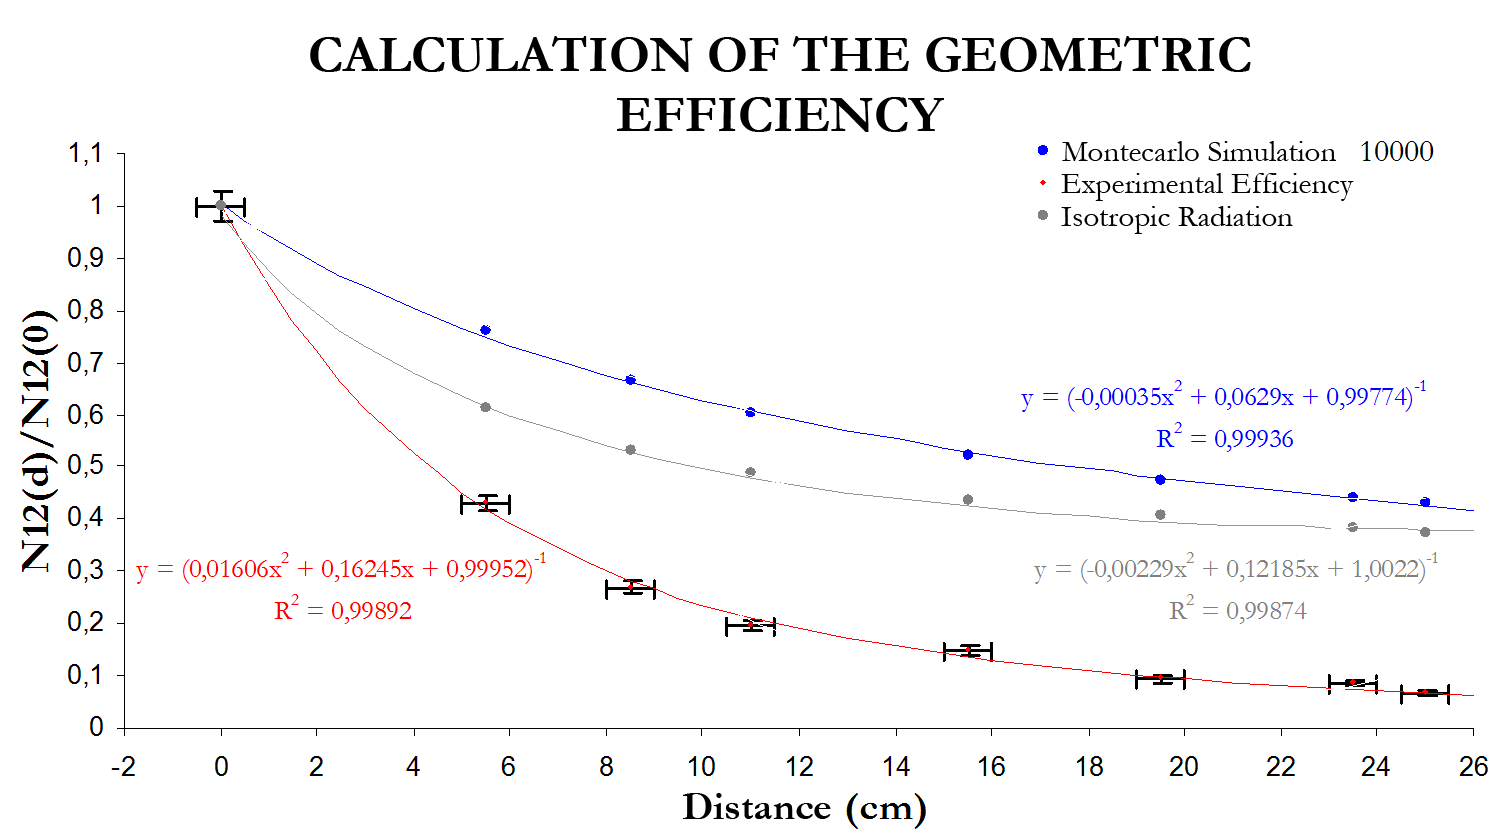
\includegraphics[width=\textwidth]{img/geoEff.png}\ec
				\caption[Comparison of experimental data with MC simulations]{Data for the MC simulation, the efficiency calculated experimentally with the error bars, and isotropic radiation. All curves are fit to curves whose dependency on the distance is proportional to the inverse square of the distance between scintillators.}\label{fig:geoeff}
			\efi

Despite the inconsistencies in values, both the curve simulation not isotropic and experimental follow a similar behavior, similar to a proportionality with $d^{-2}$.

Besides its slopes remain parallel above a large region from 6 cm more or less, where the experimental data has a lower error. This does not happen with to slope of the isotropic simulation, which is low but then comes back up.

So we can conclude that \textbf{the isotropic radiation is not a good model to represent the cosmic radiation}.

Assuming that the soft radiation has the same angular distribution as the hard one, can represent the relative fraction of hard and soft component as a function of the distance between scintillators. We can make a table of hard and soft components at different distances using the geometric efficiency calculated in this section, to be specific that obtained by MC simulation is more accurate and reliable.

Flux values for the hard and soft component obtained in the above at a distance of 30 cm section are taken into account, by correcting the geometric efficiency, and considering that, because two values were obtained for each obtained from settings for Lead and Aluminum, an average of the two will be used:

\bc
Average of the hard component at 30 cm: $J_h$ = 20 $\pm$ 2 m$^{-2}$s$^{-1}$\\
Average of the soft component at 30 cm: $J_s$ = 12 $\pm$ 4 m$^{-2}$s$^{-1}$\\
\ec
If these averages are corrected by dividing the geometric efficiency calculated by the MC for 30 cm, whose value turns out to be $\epsilon_{geo}$ = 0.3891, we obtain:

\bc
Hard component at 0 cm: $J_h$ = 51 $\pm$ 5 m$^{-2}$s$^{-1}$ = 62.2\% of the total flux\\
Soft component at 0 cm: $J_s$ = 31 $\pm$ 10 m$^{-2}$s$^{-1}$ = 37.8\% of the total flux\\
\ec

Doing the calculations, we obtain a data table like this one:


	\ctable [
	cap	    = {Comparison of the hard and soft flux for the MC and experimentf.},
 	caption = {Increasing values of d (error: $\pm$ 1 mm) with the relative fraction of hard and soft component in the case of the theoretical data and the experimental data. Calculation errors are not considered in these data.},
 	label   = {tab:MCflux},
 	pos	    = H,
	botcap
	]
	{c c c c c c c c c}
	{}
 	{\FL
		& &
		\multicolumn{3}{c}{\textbf{THEORY}} &
		\multicolumn{4}{c}{\textbf{EXPERIMENT}} \\
		\textbf{d (cm)} &
		\textbf{\pbox{.3\textwidth}{\pcen Geom.\\$\epsilon$\\[1ex]}} &
		\textbf{\pbox{.3\textwidth}{\pcen $J_h$\\[1ex](m$^{-2}$s$^{-1}$)\\[1ex]}} &
		\textbf{\pbox{.3\textwidth}{\pcen $J_s$\\[1ex](m$^{-2}$s$^{-1}$)\\[1ex]}} &
		\textbf{\pbox{.3\textwidth}{\pcen $J_d/J_s$\\[1ex]}} &
		\textbf{\pbox{.3\textwidth}{\pcen $J_h$\\[1ex](m$^{-2}$s$^{-1}$)\\[1ex]}} &
		\textbf{\pbox{.3\textwidth}{\pcen $J_s$\\[1ex](m$^{-2}$s$^{-1}$)\\[1ex]}} &
		\textbf{\pbox{.3\textwidth}{\pcen $J_d/J_s$\\[1ex]}} &
		\textbf{Error} \\
		\cmidrule(r){1-2}\cmidrule(rl){3-5}\cmidrule(l){6-9}
		0.0  & 1      & 150     & 30     & 5 & 51 & 31 & 2 & 1 \\
		5.5  & 0.7585 & 113.775 & 22.755 & 5 & 39 & 24 & 2 & 1 \\
		8.5  & 0.6647 & 99.705  & 19.941 & 5 & 34 & 21 & 2 & 1 \\
		11.0 & 0.6026 & 90.39   & 18.078 & 5 & 31 & 19 & 2 & 1 \\
		15.5 & 0.5236 & 78.54   & 15.708 & 5 & 27 & 16 & 2 & 1 \\
		19.5 & 0.4751 & 71.265  & 14.253 & 5 & 24 & 15 & 2 & 1 \\
		23.5 & 0.4398 & 65.97   & 13.194 & 5 & 22 & 14 & 2 & 1 \\
		25.0 & 0.4303 & 64.545  & 12.909 & 5 & 22 & 13 & 2 & 1
	\LL}


The ratio obtained between the hard and soft components is constant for both the tabulated data as to the experimental ones, so it follows that the angular distribution of both components is similar.

\section{Comparison of the experimental results for the flux with theory}

The table below shows a comparison between the calculated values and theory.

\begin{center}
\rowcolors{5}{lightgray}{lightgray}

	\ctable [
	cap	    = {Comparison of the hard and soft flux for the MC and experimentf.},
 	caption = {The values obtained experimentally and with the MC appear in color, a and b are the smaller and larger sides of the detectors, and d is a random separation between them.},
 	label   = {tab:thflux},
 	pos	    = H,
	botcap
	]
	{c c c c}
	{}
 	{\FL 
		\textbf{a (cm)} &
		\textbf{b (cm)} &
		\textbf{d (cm)} &
		\textbf{\pbox{.3\textwidth}{\pcen Fraction crossing both detectors (\%)\\[1ex]}} \\
		27 & 9 & 26 & 15 \\
		28 & 10 & 24 & 19 \\
		29 & 11 & 22 & 23 \\
		31 & 10 & 23.5 & 8.6 (EXP) \\
		31 & 10 & 23.5 & 43.9 (MC)
	\LL}
\end{center}

Now, since $J = J_0 \pi/2$, the total flux $J_0$  in the vertical direction, \textit{i.e.}, perpendicular to the detectors, can be calculated. From the value of the number of coincidences due to the hard and soft components obtained in the previous section, and the total flux, the following values are obtained together with their uncertainty:


	\ctable [
	cap	    = {Comparison of the flux values (theory and experiment).},
 	caption = {Theoretical values taken from \cite{prd:96} compared to those obtained experimentally.},
 	label   = {tab:thExp},
 	pos	    = H,
	botcap
	]
	{c c c c c c c}
	{}
 	{\FL
		&
		\multicolumn{3}{c}{\textbf{THEORY}} &
		\multicolumn{3}{c}{\textbf{EXPERIMENT}} \\
		\textbf{\pbox{.2\textwidth}{\pcen Flux\\(m$^{-2}$s$^{-1}$sr$^{-1}$)\\[1ex]}}&
		\textbf{Total} &
		\textbf{\pbox{.2\textwidth}{\pcen Hard\\$\sim\mu^+$\\[1ex]}} &
		\textbf{\pbox{.2\textwidth}{\pcen Soft\\$\sim e^+$\\[1ex]}} &
		\textbf{Total} &
		\textbf{\pbox{.2\textwidth}{\pcen Hard\\$\sim\mu^+$\\[1ex]}} &
		\textbf{\pbox{.2\textwidth}{\pcen Soft\\$\sim e^+$\\[1ex]}} \\
		\cmidrule(r){1-1}\cmidrule(rl){2-4}\cmidrule(l){5-7}
		\textbf{$J_0$}  &
		110 & 80 & 30 & 52 $\pm$ 9 & 32 $\pm$ 3 & 20 $\pm$ 6\\
		\textbf{$J$}  &
		180 & 130 & 50 & 82 $\pm$ 15 & 51 $\pm$ 5 & 31 $\pm$ 10
	\LL}

The obtained experimental data differ by 60\% from theory, due to the high voltage and that one of the scintillators is poorly attached to the light guide, which results in losses of photons that must reach the light guide. Furthermore, in the case of the soft component, we must take into account the absorption by the roof, which somewhat limits the amount of particles reaching the detectors.

	\chapter{Conclusions}

In this lab we will study the characteristics of a cosmic-ray coincidences detection system, that uses a scintillator-PM and NIM modules in a standard chassis, with the following settings:

\bi
	\item \textit{Time window of the system}: 50 $\pm$ 1 ns.
	\item \textit{Optimum operating point}: HV = 2200 $\pm$ 1V, V$_\text{threshold}$  = $-$200 $\pm$ 1 mV. 
	\item \textit{Estimation of spurious coincidences}: Check that their contribution is not only low but is negligible (around 0.002\%).
	\item \textit{Statistical nature}: For the time range chosen for the measurements, (between 6 and 10 minutes) the cosmic radiation should fit a Gaussian distribution with mean $\mu$ and deviation $\sigma = \sqrt\mu$, with a $\chi^2$ that has a confidence level higher than 92.6\%. For measurements below 10 s it fits well to a Poissonian distribution, whose $\chi^2$ has a confidence level of 99.8\%.
	\item \textit{Component separation}: the results at zero thickness and a distance between detectors of 30 cm are similar to these:

	\ctable [pos = H]
	{c c c c}
	{}
 	{\FL
		\textbf{(m$^{-2}$s$^{-1}$)}&
		\textbf{HARD} &
		\textbf{SOFT} &
		\textbf{TOTAL}\\
		Lead     & 19 $\pm$ 3 & 13 $\pm$ 6 & 32 $\pm$ 9 \\ 
		Aluminum & 22 $\pm$ 1 & 12 $\pm$ 2 & 34 $\pm$ 3
	\LL}

	\item \textit{Discard of the isotropic hypothesis}: The measurements must rule out that the hard radiation component has an isotropic distribution, but instead varies as a $\cos^2\theta$. Also, the ratio between hard and soft component remains constant with distance, so the soft component has the same angular distribution.
	\item \textit{Geometric efficiency}: It has been shown that there is a change in the measured radiation flux to the distance between scintillators that geom is given by the system, which has an approximately inverse quadratic dependence with distance. The MC simulation confirms this dependence made.
\ei

Final data for soft, hard and full contribution of cosmic radiation obtained experimentally and corrected by the geometric efficiency:

	\ctable [pos = H]
	{c c c c}
	{}
 	{\FL
		\textbf{(m$^{-2}$s$^{-1}$)}&
		\textbf{TOTAL} &
		\textbf{HARD} &
		\textbf{SOFT}\\
		$J_0$ & 52 $\pm$ 9  & 32 $\pm$ 3 & 20 $\pm$ 6\\
		$J$   & 82 $\pm$ 15 & 51 $\pm$ 5 & 31 $\pm$ 10
	\LL}

The sections presented can be considered as basic descriptors of the techniques that are used to determine the most important properties of cosmic radiation at ground level, and its muon component.


\section{Reflection on the main sources of error}


A difference of 200 V in the working point only makes a difference in the number of particles we count. What happens is that, depending on which phenomenon is observed, a variation like this may be significant or not.

For example, a variation of 10 particles is a variation of 10\% if we were counting  100 and now we count 90. But is a variation of 5\% if I measured 200 and now I see 190. If the experiment is dependent on detecting differences larger than 10\%, in this example the second case would be a bad place to work.

When measuring attenuation, this may have a large influence, since muons are very difficult to attenuate, and differences in the number of coincidences when increasing the thickness are very small.


\subsection{Other sources of error}

Other sources of error could be considered:
	\bi
		\item Poor contact between the scintillator and the photomultiplier. The most significant loss of particles in this experiment is the PM--scintillator transmission \cite{sou:83}.
		\item The approximation that the interaction cross section is constant, with the energy of the incident particles may not be entirely correct in certain energy ranges that may appear in the experiment.
		\item Using a counter instead of the NIM coincidences module.
		\item Treating the detectors as ideal surfaces.
		\item Assuming that the trajectories of muons are straight.
		\item Some channel of the NIM modules not working properly.
		\item The effect of the thickness of the scintillator is not taken into account in the MC simulation, and it may have some impact on the determination of the geometric efficiency, even if it has an exponential effect, such that $J_\text{final} = J_\text{initial} e^{- x / l}$, where $l$ is the mean free path of the particles in the detector. However it is fine to take this into account only in very large detectors, which is not the case in this experiment.
		\item The thickness of the layers is not the sum of the thicknesses, there are air-filled spaces, although the air really has very little effect on the incident particles, as demonstrated on a small calculation performed on the relevant section of chapter \ref{chap:exp}.
		\item Coincidences cables being damaged or not of the same size...
		\item ...etc.
	\ei


	\bc* * *\ec

The effect of other sources that your lab mates who work near the site of measurement may be using is negligible. Furthermore, these sources will be mostly sources of alpha, beta and gamma radiation, whose range both in Pb and Al is very small.

Of course you could also consider effects as warming of the conductors by Joule effect, inhomogeneous magnetic fields, etc. These factors taken separately are of systematic nature, however the influences are so complex that they can produce global effects in both directions and in variable entities, so that the corresponding errors become random.



	% Appendixes ---------------------------------------------------------------
	%	 Title aligned right and in italics with chapter number
	\titleformat{\chapter}[block]{\raggedleft\itshape}{}
		{0pt}{\parbox{\linewidth}{\raggedleft\vspace*{1em}\Huge \chaptername~\thechapter: #1}}

	\appendix
	\renewcommand\chaptername{Appendix}
	\renewcommand{\theequation}{\Alph{chapter}.\arabic{equation}}
	\setcounter{equation}{0}    % reset counter
	\addtocontents{toc}{\protect\hrulefill\par}
	\cleardoublepage
\chapter{The flux integral}\label{chap:app1}

As discussed in the Theoretical Introduction, the distribution of cosmic radiation is not isotropic, but it depends on the altitude, longitude and latitude.

For example, muons reach the ground with an average energy of $\sim$4GeV \cite{eid:04}. The angular distribution of muons at ground level has the following characteristics:
\bi
	\item It's proportional to $\cos^2\theta$ for muons of energy $E_\mu \sim$ 3GeV, with $\theta$ being the zenith angle,
	\item At lower energies the angular distribution becomes steeper,
	\item It saturates at higher energies, 
	\item for $E_\mu \gg \epsilon_\pi$, the distribution has the shape of $\sec\theta$.
\ei

In the range of energies with which the muons reach the ground, their angular distributions can be described by the equation:

		\be J(\theta,\varphi) = \frac{d^3N}{dA \,dt \,d\Omega} = J_0 \cos^2\theta \frac{part.}{m^2 \,s \,sr}\ee

where
    $J$ is the total $\mu$ flux per unit area, per unit time and per unit solid angle,
	$\theta$ is the zenith angle, which varies between $-\pi$/ 2 and $+\pi$/ 2, depending on the configuration of our system,
	$\varphi$ is the azimuth angle, which varies from 0 to 2$\pi$, and 
	$J_0$ is the flux in the vertical direction per horizontal unit area per unit time and per unit solid angle.

The presence of the cosine function accounts for the fact that we have \textit{non-isotropic radiation}. Due to the presence of the cosine, the above expression has a maximum in $\theta = 0$, that is, in the vertical and perpendicular direction to the plane of the detectors, from where it is concluded that $J_0$ is the vertical flux direction.

In this case we have a flat detector surface, and the unit of area is not always oriented horizontally to the direction of incidence.

	\noindent\begin{minipage}{.5\textwidth}
$\quad$ A unit area of m$^2$ is set. To calculate the flux coming from all directions and across the whole surface of the detector, we must integrate through all the solid angle:

	\bc $d\Omega = \sin\theta \,d\theta \,d\varphi$ \ec

and take into account that the differential element of area that the scintillator actually presents for the reaction is:
	\end{minipage}%
	\begin{minipage}{.5\textwidth}
	\bfi[H]
		\bc
			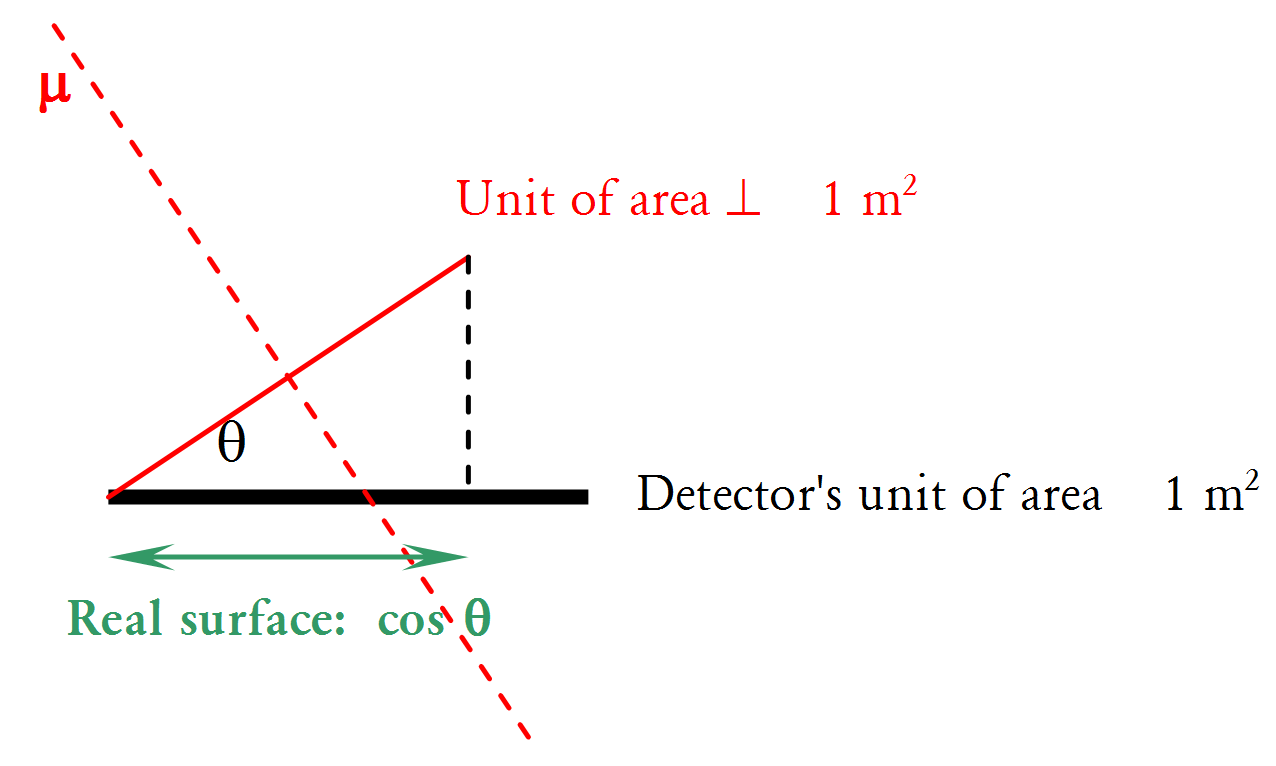
\includegraphics[width=.9\textwidth]{img/app1.png}
			\captionsetup{width=0.8\textwidth}\caption
				[Schematic view of the incident particle path.]
				{Schematic view of the incident particle path.}\label{fig:app1}
		\ec
	\efi
	\end{minipage}\captionsetup{width=0.8\textwidth}



	\bc $dA = dS \cos\theta$ \ec

\textit{i.e.} solve the following integral:

	\be
		\begin{split}
			I &= \int J \,dA \\
			  &= \int_0^S \left| j(\theta,\varphi) \right| \,dS \,\cos\theta \\
			  &= \int_0^S\int_0^{2\pi}\int_0^{\pi/2} J_0 \,\cos^3\theta \sin\theta \,d\theta \,d\varphi \,dS \\
			  &= J_0 \,2\pi S \int_0^{\pi/2} \cos^3\theta \sin\theta \,d\theta
		\end{split}
	\ee

The last integral, which only has dependence on $\theta$, is easily solved by:

	\be
		\begin{split}
			\int_0^{\pi/2} \cos^3\theta \sin\theta \,d\theta &= 
			\int_0^{\pi/2} \left[ -\frac{1}{4}\frac{d(\cos^4\theta)}{d\theta}\right] d\theta \\
			&= \frac{1}{4}\int_0^1 d(\cos^4\theta) \\
			&= \frac{1}{4} 
		\end{split}
	\ee

thus obtaining:

	\be I = J_0 \,\frac{\pi}{2}S\frac{part.}{s} = \frac{N}{t}\ee

which is simply the total intensity of particles per unit time reaching the scintillator detector with rectangular geometry and surface $S$, and equals the number of counts per unit time to be registered in it (after noise substraction).

For the soft component we can assume to a first approximation that the distribution is equal to that of the hard component.

	\cleardoublepage
\chapter{Monte Carlo}\label{chap:app2}

In this appendix we will try to explain the code of the simulation program, which uses the Monte Carlo method to calculate the geometric efficiency of the detectors. In this case we have used the C programming language. This appendix also explains the geometry of the system, which is shown in Fig. \ref{fig:app2}. The code is included at the end.

The first lines of code ask for the input data (the distance between scintillators and the number of muons to be simulated). The dimensions of the scintillators are fixed to 10$\times$31 cm, which are the dimensions of the scintillators at the lab. The algorithm is as follows:

\ben
	\item The program generates a stream of particles through a \code{for} loop, where they are simulated one by one. Each particle strikes the upper detector in random positions given by the triad $(x, y, z)$, that follow a random angular distribution typical of cosmic radiation, given by $cos^4\theta$\footnote{Where $\theta$ is defined in spherical coordinates.} (Appendix \ref{chap:app1}).

	\item For the random number generation, the program uses the C function \code{rand()}, which generates random numbers with values between 0 and \code{RAND\_MAX} = 32768. According to Fig. \ref{fig:app2}, the initial positions on the scintillator 1 are given by:
	\bi
		\item $x \in [0, x_s]$, where $x_s$ is the width of the scintillator, so $x = x_srand()$
		\item $y \in [0, y_s]$, where $y_s$ is the length of the scintillator, so $y = y_srand()$
		\item $z = d$, where $d$ is the distance between scintillators.
	\ei

	\item Then, the direction of incidence ($\theta$, $\varphi$) is generated. This is the direction whith which the particle exits the first detector. It must be taken into account that the angle $\theta$ grows from $-\pi / 2$ to $+\pi / 2$\footnote{This is the incidence angle. Note that there is symmetry between what goes above and below the scintillator.}. The muon reaches the second detector at position $(x', y', z')$. If the projection of $(x, y, z)$ on the plane is given by $\rho$, the projection on the plane from point $P$ to point $P'$ is $\rho''$, which depends on the direction of incidence as:

	\bc$\rho' = d\,\tan\theta$\ec

where $\tan\theta$ is calculated from a $\cos\theta$ generated as the fourth root of a random number between 0 and 1 (App. \ref{chap:app1}), so that we give the correct angular weight to our distribution:

	\bc
		$\cos\theta = \sqrt[4]{\code{rand()}}$

		$\sin^2\theta = \sqrt{1 - \cos^2\theta} \quad \rightarrow \quad$
		$\tan\theta = \frac{\sqrt{1 - \cos^2\theta}}{cos\theta}$
	\ec

Since the system has azimuthal isotropy, the $\varphi$ coordinate is generated in the following way:

	\bc $\varphi \in [0, 2\pi], \quad \rightarrow \quad \varphi = 2\pi\,\code{rand()}$ \ec

	\item After crossing the lower scintillator, the impact point is simulated. The position of the particle in the lower detector is given by the sum of two vectors, one is the projection of the initial position $(x, y, z)$ on the plane ($\rho$), and the other is the vector $\rho'$ mentioned above, as shown in Fig. \ref{fig:app2}, so that its new coordinates on the second scintillator will be:

	\begin{equation*}
		\begin{split}
			x' &= x + \rho'cos\varphi\\
			y' &= y + \rho'sen\varphi\\
			z' &= 0.
		\end{split}
	\end{equation*}

	\item Once the new positions on the lower detector are calculated, they may fall within or outside its limits depending on the angular distribution they have. Applying the correct condition, the program will count how many times it succeeds in collecting each particle. This condition is:

	\graybox{.8}{.7}{\enquote{If $x \in [0, x_s]$, and $y \in [0, y_s]$, (that is, if the two conditions are fulfilled simultaneously) then count one.}}

The value of the counts is stored in a variable with each iteration of the \code{for} loop, and when the loop is finished the program calculates the geometric efficiency as the ratio between this variable and the initial number of particles.
\een

	\bfi[H]
		\bc
			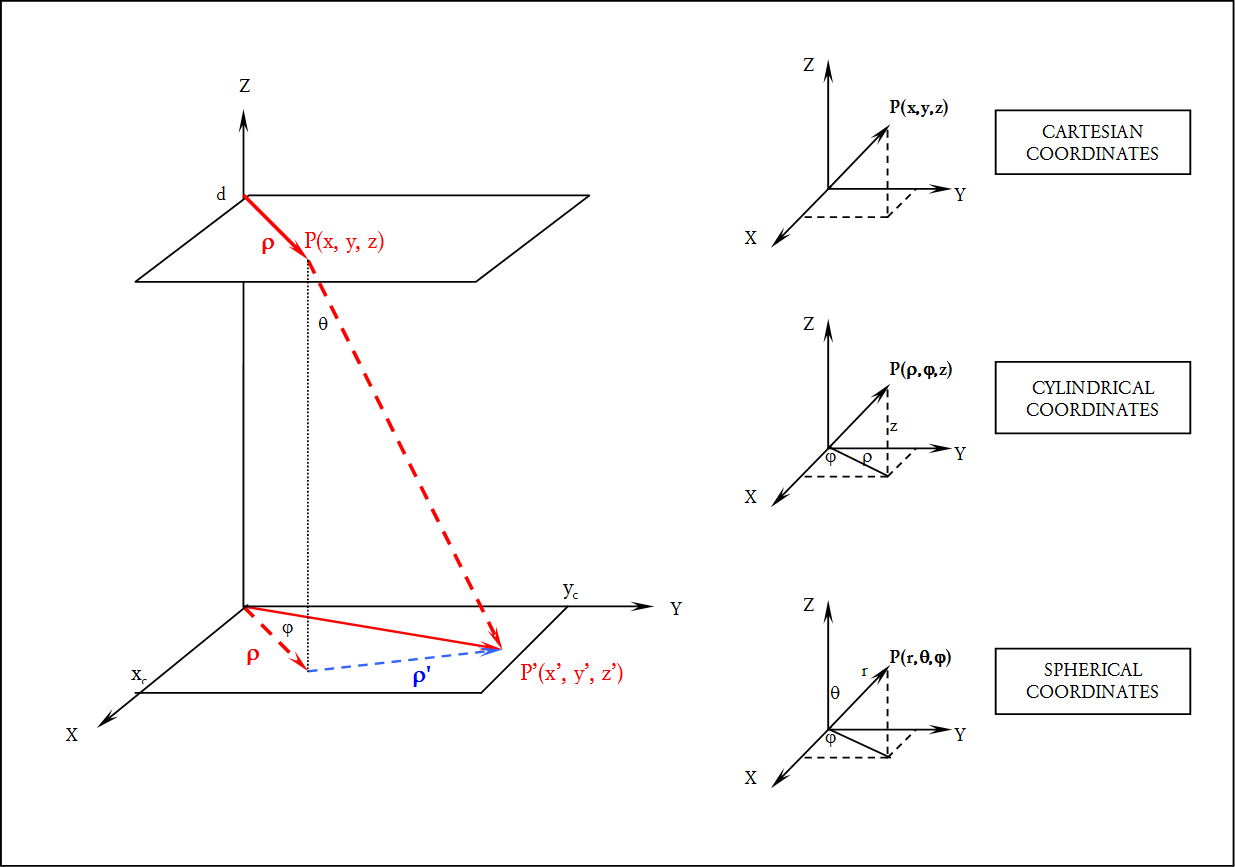
\includegraphics[width=.9\textwidth]{img/app2.png}
			\caption
				[geometry used to simulate the setup used in the laboratory.]
				{On the left, the geometry used to simulate the setup used in the laboratory. The coordinates of a particle that arrives to the upper detector at point $P$, and then moves to point $P'$ of the lower detector, are a combination of Cartesian, Cylindrical and Spherical coordinates. The angular coordinate $\theta$ shown in the figure on the left is the angle of incidence, not to be confused with the coordinate $\theta$ of the Spherical coordinates.}\label{fig:app2}
		\ec
	\efi

Once the efficiency is calculated for one detector, it is known for the other, since we made the approximation that the scintillators are similar.

In the case of an \textit{isotropic distribution}, the problem's geometry does not change, only the angular distribution, and the same program can be used modifying the line:
	
\lstinputlisting[
	firstnumber = 49,
	firstline   = 49,
	lastline    = 49
]{../mcEff/mcScin.c}

for:

\lstinputlisting[
	firstnumber = 49,
	firstline   = 49,
	lastline    = 49
]{../mcEff/mcScinIso.c}

Below, the code is shown:

\lstinputlisting{../mcEff/mcScin.c}


	\cleardoublepage
\chapter{Error handling}\label{chap:app3}


This appendix tries to explain the basics of error handling that have been cited during the text used in the analysis of the data.


\section{Calculating uncertainties}\label{sec:unc}

\ben
	\item \textbf{Error of direct measurements:}\\[12pt]
In direct measurements, it is assumed a pattern as a unit of measurement, and the measurements are performed by comparison. If a magnitude $x$ is measured and an uncertainty is assigned to that measurement, the value could have values between $x_a$ and $x_b$ with equal probability. In these cases the measured value is the average value of both $\bar{x}$, and as $\delta_x$ is the difference, which is often cconsidered as error, although it is not randomized \cite{san:89}.

\be \bar{x} = \frac{x_a + x_b}{2} \quad \delta_x = \frac{ \left| x_a - x_b \right| }{2}\ee

The value of $\delta_x$ is always positive by definition.

	\bi
		\item \textit{Absolute error}: The measured value is offered as $\bar{x} \pm \delta_x$, with $\d_x \ll \left| x \right|$.
		\item \textit{Relative error}: $\epsilon(x) = \frac{\delta_x}{\left|x\right|} \ll 1$ It is expressed in \% if it was already multiplied by 100. Although it depends on the particular case, it is estimated that a relative error of $\geq$ 10\% is poor, and $\leq$ 1\% is good.
	\ei

	\item \textbf{Error of indirect measurements:}\label{item:ind}\\[12pt]
The indirect measurements presented here were obtained as a function of other measurements and are considered to be absolute. Its unit of measurement is also a function of the other units of measurement.

	\bi
		\item \textit{Error propagation}: If we want to determine the error of a variable that is a function of others, we must apply the Taylor series \cite{san:89}:

		\bi 
			\item One variable: 
				\be\begin{split}
					z = q (x) 
					&\quad\rightarrow\quad q\left(x + \Delta x\right) = q(x) + \frac{dq}{dx}\Delta x + \dots \\
					&\quad\rightarrow\quad \delta(z) = \left| \frac{\delta q}{\delta x} \right|
				\end{split}\ee
			\item Several variables:
				\be z = q (x, y, \dots) \quad\rightarrow\quad 
					\delta(z) = \left| \frac{\delta q}{\delta x} \right|\delta x + 
								\left| \frac{\delta q}{\delta y} \right|\delta y + \dots
				\ee
		\ei
	\ei

	\item \textbf{Error of measurements with calibrated equipment:}\\[12pt]
Those provided by the relevant manufacturer. They are taken from the manuals.

	\item \textbf{Rounding:}\\[12pt]
All $\delta x$ error is estimated and is subject to uncertainty, so \textbf{\textit{it is enough to use one significant figure}} in the result. Therefore, the measured value $x$ is rounded up to the last significant figure present in its $\delta x$.

	\bi 
		\item \textit{Rounding rules}:
		\bi
			\item If the figure is $<$ 5 is it eliminated.
			\item If the deleted figure is $>$ 5, the last retained figure is increased by one.
			\item If the deleted figure is = 5, the nearest even number is taken as the last digit, if it is odd, the higher is taken.
		\ei

		\item Also, take the following remarks into account \cite{san:89}:
		\bi
			\item In additions and subtractions, the result has no more significant digits after the decimal sign than the value with lower number of significant decimal digits.
			\item In multiplications, divisions, and roots, the result takes no more significant digits than the value with the lower number of them.
		\ei
	\ei


	\item \textbf{Random errors:}\\[12pt]

	\bi
		\item \textit{One variable}:
If the same measurement is repeated many times ($n$) it presents a variation called \textit{dispersion}. If the histogram is constructed, the best value is the \textbf{\textit{mean}}, and the error is the \textbf{\textit{deviation}} around it.

		\be \bar{x} = \frac{\sum_i^n x_i}n, \qquad Mean\ Devation = \frac{\sum_i^n \left| x_i - \bar{x} \right|}n\ee

The best value of $x$ is obtained as the value of $m$ that minimizes the expression:

		\be \frac{\sum_i^n \left| x_i - m \right|}n\ee

but since the derivative of the absolute-value function is not continuous, \textbf{\textit{variance}} is used instead:


		\bc\begin{minipage}{.3\textwidth}
			\bc\AlegreyaSansSC\color{gray} Variance\ec
		\end{minipage}%
		\begin{minipage}{.5\textwidth}
			\graybox{.9}{.8}{\be S^2 = \frac{1}{n}\sum_i^n \left( x_i - \bar{x} \right)^2 \ee}
		\end{minipage}\ec

		\bc\begin{minipage}{.3\textwidth}
			\bc\AlegreyaSansSC\color{gray} Standard Deviation\ec
		\end{minipage}%
		\begin{minipage}{.5\textwidth}
			\graybox{.9}{.8}{\be S = \sqrt{S^2} \ee}
		\end{minipage}\ec

		\bc\begin{minipage}{.3\textwidth}
			\bc\AlegreyaSansSC\color{gray} Corrected Standard Deviation\ec
		\end{minipage}%
		\begin{minipage}{.5\textwidth}
			\graybox{.9}{.8}{\be S_{n-1} = \sqrt{\frac{1}{n-1}\sum_i^n \left( x_i - \bar{x} \right)^2} \ee}
		\end{minipage}\ec

The corrected standard deviation is used when $n$ is small, and $n-1$ are the degrees of freedom (the values minus the mean calculated from them).\\

If not one, but a set of measurements of the same variable, are repeated several times (for example, 10 experiments of 3 measurements each), we can calculate the variance and the corrected standard deviation of the mean as:

		\bc\begin{minipage}{.3\textwidth}
			\bc\AlegreyaSansSC\color{gray} Variance\ec
		\end{minipage}%
		\begin{minipage}{.5\textwidth}
			\graybox{.9}{.8}{\be S^2(\bar{x}) = \frac{1}{n^2}\sum S^2(x_i) = \frac{S^2(x)}{n} \ee}
		\end{minipage}\ec

		\bc\begin{minipage}{.3\textwidth}
			\bc\AlegreyaSansSC\color{gray} Corrected Standard Deviation of the mean value\ec
		\end{minipage}%
		\begin{minipage}{.5\textwidth}
			\graybox{.9}{.8}{\be S(\bar{x}) = \frac{S(x)}{\sqrt{n}} \ee}
		\end{minipage}\ec

What these expresions tell us is, that it is worth repeating the experiments a number of times, since 1 /$\sqrt{n} \ll$ 1 / $n$. However, there comes a time when the decrease in error (which follows a root-function tendence), is not worth the effort.

		\item \textit{Several variables}:
Given two variables $x$ and $y$, the \textbf{\textit{covariance}} of $x$ and $y$ is defined as:

		\be S(x,y) = \frac{ \overset n{\underset i{\sum}} (x_i - \bar{x})(y_i - \bar{y})}{n} \ee

  where $\left| S(x,y) \right| \ll S(x)S(y)$, and if $x$ and $y$ are independent,

$S(x,y) \xrightarrow[n \rightarrow \infty]{} 0$.\\[12pt]

If we have a function like $z = q (x, y)$, the variance is given by:

		\graybox{.9}{.8}{%
			\be S^2(z) = \left( \frac{\partial q(x,y)}{\partial x} \right)^2 S^2(x) + 
						 \left( \frac{\partial q(x,y)}{\partial y} \right)^2 S^2(y)\ee
		}
	This expression is less pessimistic than $\delta z$ (\ref{sec:unc}--\ref{item:ind}) for small errors, but more for large errors.

	\ei
\een

\section {Classification of errors}

\ben
	\item \textbf{Systematic:} When they happen repeatedly, they affect the results always in the same direction \cite{gia:75}.
	\bi
		\item \textit{Bad calibration}: 
Needles in the wrong position, measurement scale too big, poor internal calibration of electronic equipment, miscalibration by faulty construction, friction on the axes of moving parts, elastic hysteresis of the springs of suspension wires, etc.

		\item \textit{Poor conditions}:
When the conditions of pressure, temperature, etc. are not compatible with the specifications of the manuals.

		\item \textit{Imperfect techniques}:
It depends on the experience of the experimenter. For example, when measuring the spring constant, if the mass is increased by removing and placing again the weights each time, instead of gradually increasing them. This is a mistake because the spring gets shrinked and stretched.

		\item \textit{Incorrect formulas}:
When the measurements must have a certain number of significant digits, but formulas with certain ideal approximations are used.
	\ei

	\item \textbf{Casual}: When it is not possible to determine its cause, they are unpredictable.
	\bi
		\item \textit{Assessment errors}:
If the same person performs the same measurement many times, they won't measure the same value. This has to do with the estimation they make of a certain fraction of the smallest division of the measuring scale.

		\item \textit{Working conditions}: Environmental conditions, someone opens a tap or closes a door, planetary configurations, etc.

		\item \textit{Lack of definition}: When the quantity to be measured is not fully defined, for example, the radius of a sphere of metal, since its surface has microscopic imperfections.
	\ei

	\item \textbf{Illegitimate}: Distraction, fatigue.
	\bi
		\item \textit{Personal}: Poor reading, incorrect adjustment of the conditions of a device, preliminary calculations poorly executed.

		\item \textit{Calculation-wise}: Computers or programs without sufficient precision.

		\item \textit{Chaotic}: When the effect of a disturbance is greater than the possible casual error.

		\item \textit{Random}: These are the combination of many small and unknown causes. Several measurements must be performed or several different instruments must be used.
	\ei
\een

\section{Definitions}

\begin{description}
	\item[Precision:] \hfill \\
The smaller the casual errors are, the the more precise a measurement is.

	\item[Accuracy:] \hfill \\
The smaller the systematic errors are, the more accurate a measurement is.

	\item[Sensitivity:] \hfill \\
(Associated with the measuring device) Ability of an instrument to detect small variations in the measured variable.
\end{description}

	\cleardoublepage
\chapter{Statistical Distributions}\label{chap:app4}

Much of the problems in physics can be described, at least approximately, with a small group of theoretical statistical distributions characterized by a \textbf{\textit{probability density function $P(x)$}}, which provides the expected frequency of a particular random event happening.

This appendix will proceed to explain the salient features of the statistical distributions to which the data taken in this experiment fit. In particular, the \textbf{Normal or Gaussian} distribution, the \textbf{Poisson} distribution and the \textbf{Chi-square} distribution are discussed.


\section{Normal or Gaussian distribution}\label{sec:gauss}

Most natural phenomena fit a Gauss \enquote{bell} curve, so is also known as \textit{Normal Distribution}. Accurately describe any population whose randomness is due to an effect that can be decomposed into the sum of a large number of independent causes. It applies to a population of CONTINUOUS random variable. Instrumental errors are well described by a Gaussian curve.

The Gaussian distribution is a mathematical simplification of the  \textbf{\textit{Bernoulli or Binomial Distribution}} when the number of trials $N$ is very large ($\gg$ 30). The probability that in each test the obtained value is one of two given values is not very small potential ($\geq$ 0.05). The probability of obtaining a value $x$ is:

	\be P(x) = \frac{1}{\sigma\sqrt{2\pi}} \,e^{\frac{\left(x-\mu \right)^2}{2\sigma^2}}\ee

where $\mu$ is the mean and $\sigma$ the standard deviation, which is the width of the distribution at $\sim$60\% of the overall height, although sometimes the full width at half height is used: FWHM = 2.35$\sigma$. This distribution is CONTINUOUS, SYMMETRICAL around the mean value, and NORMALIZED with TWO parameters, $\mu$ and $\sigma^2$.

We must clarify that the expected value of the random variable $x$ is defined as: $E [x] = \int x \,P(x) \,dx = \,<x>$ and is also called \textit{average} or \textit{mean value} of $x$, which is usually denoted as: $\mu = E [x]$, and refers to the theoretical distribution $P(x)$, so it should not be confused with the average experimental value of a sample that is mentioned in Appendix \ref{chap:app3}.

This distribution is centered in $\mu$, where it has its maximum. It normalization factor is $1/\sigma\sqrt{2\pi}$ so that the integral of $P(x)$ in the entire sample space is 1, and its width is given by $1/2\sigma^2$, so that the bigger the $\sigma$, the greater the width. The two inflection points are given by $\mu \pm \sigma$. The usual notation is $N(\mu, \sigma)$.

Important parameters:
	\bi
		\item $\left\langle x \right\rangle = \mu$ mean (matches mode).
		\item $\left\langle(x - \mu)^2\right\rangle = \sigma^2 = \bar{x^2} - \mu^2$ variance.
		\item $\sigma$ Standard deviation.
	\ei

The probability of obtaining a value of $x$ less than one particular $x_c$ is given by the integral:

	\be P(x < x_c) = \int_{-\infty}^{x_c} P(x) \,dx \ee

As this integral is difficult to solve, the following approximation is used:

	\be P(x < x_c) = 1 - \frac{1}{\sqrt{2}\pi} \,e^{-\frac{1}{2}\left( \frac{x_c - \mu}{\sigma}\right)^2} \left[ a_1t + a_2t^2 + a_3t^3 + a_4t^4 + a_5t^5\right] \ee\vfill

\bc
\begin{minipage}[t]{.4\textwidth}
	\bc with\ec
	\begin{equation*}
		t = \frac{1}{1 + a_0 \left(\frac{x_c - \mu}{\sigma}\right)}
	\end{equation*}
\end{minipage}%
\begin{minipage}[t]{.6\textwidth}
	\bc and\ec
	\begin{equation*}
		\begin{split}
			a_0 &= \text{0.2316419}   \\
			a_1 &= \text{0.31938153}  \\
			a_2 &= -\text{0.356563782}\\
		\end{split}\quad
		\begin{split}
			a_3 &= \text{1.78147937}  \\
			a_4 &= -\text{1.821255978}\\
			a_5 &= \text{1.330274429} \\
		\end{split}
	\end{equation*}
\end{minipage}
\ec

A similar approach is used in the program used to calculate the confidence level of $\chi^2$. See the code at the end of this appendix.

	\bfi[H]
		\bc
			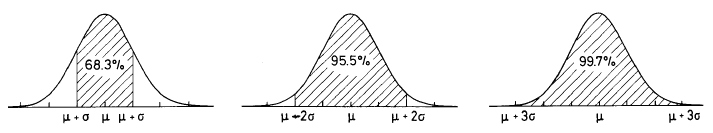
\includegraphics[width=.9\textwidth]{img/app41.png}
			\caption
				[Confidence intervals.]
				{Confidence intervals:\\
					$x = \mu \pm  \sigma \rightarrow$ 68.3\% ($\sim$2/3 of the data)\\
					$x = \mu \pm 2\sigma \rightarrow$ 95.4\%\\
					$x = \mu \pm 3\sigma \rightarrow$ 99.7\%.}\label{fig:confidence}
		\ec
	\efi


	

\section{Poisson distribution}\label{sec:poisson}

Sometimes an observation consists of counting objects. We always count in relation to a range that can be time, length, area, etc.

The Poisson distribution applies to \enquote{rare} events. It describes DISCRETE  processes in which the observation of a single event is very unlikely, but the number of trials is so large that at the end there is a reasonable number of events.

It is also considered to be a limit of the Binomial distribution when the number of trials is very large and the probability of each test the obtained value is one of two possible values is very small. For example, in radioactive decay, if small time-measurement intervals are taken and compared with the average life of the source, where the number of nuclei $N$ is large, the probability of getting a value $x$ times can be obtained as follows:

\bi
	\item Probability of having an event per unit interval: $\lambda$ (very small).
	\item Probability of having an event within an interval $dt$: $\lambda \,dt$.
	\item In an interval $t$, the average of events is: $\mu = \lambda t$.
\ei

The basic assumption is that the $\lambda$ probability is so small that in the interval $dt$ two or more events can not occur:

\bi
	\item Chance of having 2 events within a time interval $dt$: $p_2 (dt) = O$.
	\item Probability to have O events within a time interval $dt$: $p_0 (dt) = 1 - \lambda \,dt$.
	\item Probability of having $x$ events within an interval $t + dt$:\\
 $p_x (t + dt) = p_x (t) (1 - \lambda \,dt) + p_{x-1} (t) \,\lambda \,dt$.
\ei


If now we subtract $p_x (t)$ on both sides of the last expression we obtain:

\be
	\begin{split}
		\frac{dp_x(t)}{dt} = &\lambda\left( p_{x-1} - p_x \right)	\quad
		\rightarrow	p_x = \frac{\left(\lambda t \right)^x}{x!} \,e^{\lambda t}\\
		&P(x) = \frac{\mu^x}{x!}e^\mu					\quad
		x = 0, 1, 2 \dots
	\end{split}
\ee

This would be the probability that the random variable takes the value $x$. This distribution is DISCRETE, NORMALIZED and ASYMMETRIC with respect to the mean, with a SINGLE parameter, $\mu$.

Important parameters:
	\bi
		\item $\mu = \overset\infty{\underset 0{\sum}} x P(x)$ mean (matches mode).
		\item $\sigma^2 = x^2 - \mu^2$ variance.
		\item $\sigma = \sqrt{\mu}$ Standard deviation.
	\ei


This indicates that if random events are counted, it is very difficult to obtain high accuracy. For a $\sigma\sim$1\%, 10,000 events would be needed. When we perform an experiment of counting random events and obtain a value $x$, the result with its error is: $x ± \sqrt{x}$.

If the average is increased, the probability distribution moves to the right and its shape becomes more symmetric and flat. When the numbers are large, the Poisson distribution becomes a Gaussian distribution with $\sigma = \sqrt{\mu}$, so we have a particular case of Gaussian that depends on a single parameter: the mean $\mu$.

	\bfi[H]
		\bc
			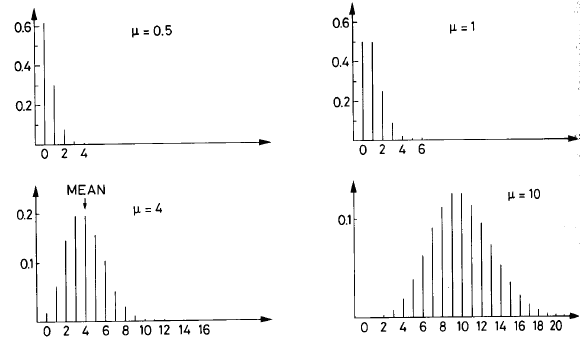
\includegraphics[width=.9\textwidth]{img/app42.png}\\
			\caption
				[Limit of a Gaussian distribution.]
				{The limit of a Poisson distribution is a Gaussian:\\
				${\color{white}.} \qquad {\color{white}.} \qquad P(x) = \frac{1}{\sqrt{2\pi\mu}} \,e^{\frac{(x - \mu)^2}{2\mu}} $\\
This result is very important because it indicates that the result of having a large number of events is no different from the result of measuring a continuous variable.}\label{fig:poisson}
		\ec
	\efi

The probability of obtaining a value of $x$ that is lower than one particular $x_c$ is given by the sum:

	\be P(x \leq x_c) = \sum_0^{x_c} \frac{\mu^k}{k!} \,e^\mu \ee

The values ​​of the Poisson distribution function calculated with this expression are shown in the following tables:

	\bfi[H]
		\bc
			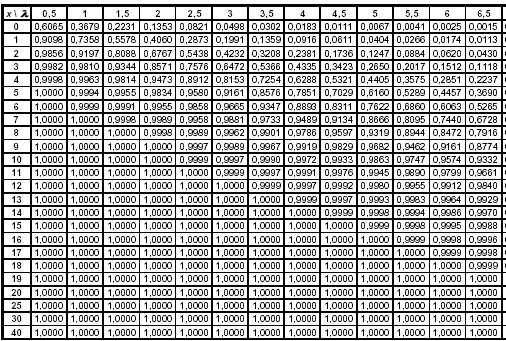
\includegraphics[width=.9\textwidth]{img/app43.png}\\[12pt]
			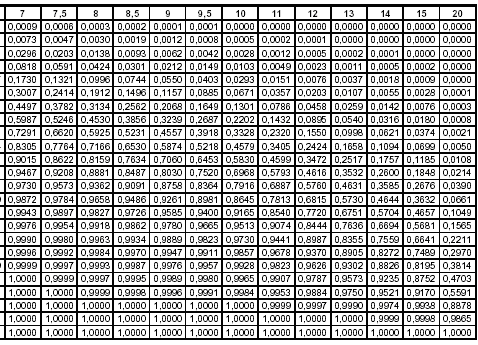
\includegraphics[width=.9\textwidth]{img/app44.png}\\
			\caption
				[Limit of a Gaussian distribution.]
				{Values ​​of the Poisson distribution for a certain value of $x$ and for a given value of the mean (here designated by $\lambda$).}\label{tab:tables}
		\ec
	\efi

\section{Chi-squared distribution}\label{sec:chi2}

It is particularly useful for estimating the so called \textit{goodness} of the fit of the experimental data when compared with the theoretical distribution formulas.

The shape of this distribution is deducted below: Suppose there are $n$ independent variables $x_i$ with \textit{normal} distributions of mean values $\mu_i$ and ​​standard deviations $\sigma_i$,  with:

	\be \chi^2 = \sum_i^n \frac{(x_i - \mu_i)^2}{\sigma^2}\ee

The probability that $x_i$ is between $x_i$ and $dx_i$ is:

	\be
		\begin{split}
			P(x_1x_2\dots x_n) \,dx_1 \,dx_2\dots\,dx_n 
			&= P(x_1)P(x_2)\dots P(x_n) \,dx_1 \,dx_2\dots\,dx_n \\
			&= \frac{1}{\sigma_1\sigma_2\dots\sigma_n(2\pi)^{n/2}} \,e^{-\frac{\chi^2}{2}}
		\end{split}
	\ee

The probability that $\chi^2$ 
is between $\chi^2$ and $\chi^2 + \,d\chi^2$ 
is $e^{-\frac{\chi^2}{2}}\chi^{n-1} \,d\chi$, 
where $\chi^{n-1} \,d\chi$ 
is the volume between two spheres of radius $\chi^2 + \,d\chi^2$ 
in an n-dimensional space. Manipulating this expression, integrating over all space to find the normalization constant, and replacing $n$ by $\nu$ (the degrees of freedom) we obtain:

	\be
		P(\chi^2) = \frac{\left(\frac{\chi^2}{2}\right)^{\frac{\nu}{2}-1}}%
						 {2\Gamma\left(\frac{\nu}{2}\right)}% 
					e^{-\frac{\chi^2}{2}}
	\ee

where $\Gamma$ is the Gamma function of Euler, which is defined as:

	\be
		\Gamma\left(\frac{\nu}{2}\right) =
		\left\{%
			\begin{array}{l}
				\left(\frac{\nu}{2}-1\right)!\\
				\sqrt{\pi}
				\left(\frac{1}{2}\right)
				\left(\frac{3}{2}\right) \dots 
				\left(\frac{\nu}{2} - 1\right)
			\end{array}
			\quad
			\begin{split}
				&\text{ for\ even\ }\nu\\
				&\text{ for\ odd\  }\nu
			\end{split}
		\right.
	\ee

	\bfi[H]
		\bc
			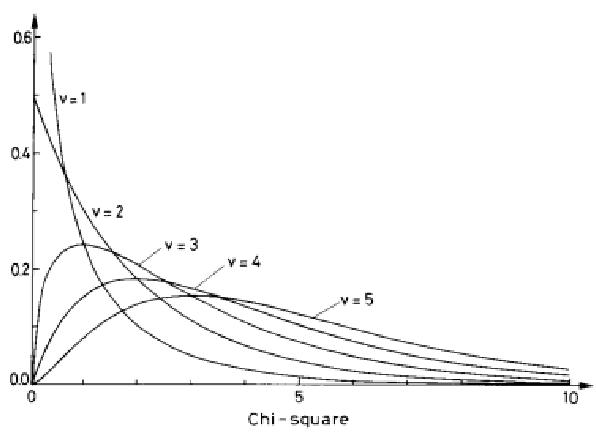
\includegraphics[width=.9\textwidth]{img/app45.png}
			\caption
				[Chi-squared distribution.]
				{Chi-squared distribution.}\label{fig:chi2}
		\ec
	\efi

This distribution is ASSYMETRIC, with a SINGLE paremeter $\nu$ that determines the shape of the distribution.

Important parameters:
	\bi
		\item $\chi^2 = n - 2$ most probable value.
		\item $\mu = \,<\chi^2> = n$ mean value.
		\item $\sigma^2 = 2n$ variance.
		\item $\sigma(\chi^2) = \sqrt{2n}$ standard deviation.
	\ei

If the variables are not independent, $n$ is changed by $\nu = n - k$, where $\nu$ represents the degrees of freedom, and $k$ is the number of constraints in the system.

The $\chi^2$ of a fit has a $\chi^2$ distribution with $\nu$ degrees of freedom and a constraint, which can be rewritten as:

	\be\chi^2 = \frac{(n-1)s^2}{\sigma^2}\ee

where $s^2$ is the best sample estimate of the population variance of the $n$ variables, and:

	\be \sigma(s^2) = \sqrt{\frac{2}{n - 1}} \sigma^2 \ee

is the standard deviation of the sample variance $s^2$ if $\sigma^2$ is known for a normal universe.

The probability of obtaining a value of $\chi^2$ that is lower than one particular $\chi_c^2$ is given by the integral:

	\be
		P\left(\chi^2 < \chi_c^2\right) =
		\int_{-\infty}^{\chi_c^2} P_\nu(x) \,dx
	\ee

Since this integral is very difficult to solve, this approximation used instead:

	\be
		\begin{split}
			P\left(\chi^2 < \chi_c^2\right) &= \frac{2\chi_c^2}{\nu} P_\nu(\chi^2)
			\left[1 + \sum_{k=1}^\infty \frac{\chi^{2k}}{(\nu + 2)(\nu + 4)\dots(\nu + 2k)}\right]\\[12pt]
			Q\left(\chi^2 < \chi_c^2\right) &= 1 - P(\chi^2 < \chi_c^2)
		\end{split}
	\ee

If we pick a particular $\chi_c^2$ and compare it with the $\chi^2$ of the fit to be evaluated, three cases can occur:

\bi
	\item If $\chi^2 \in [0, \chi_c^2)$ it is possible to say that the fit is good,
	\item If $\chi^2 \in [\chi_c^2, \infty)$ it is bad,
	\item If $\chi^2 = \chi_c^2$ this criteria doesn not decide.
\ei


In addition, the judgment made deserve a certain confidence as a percentage that must be previously chosen. If we choose a confidence level of 95\%, 0.05 is the probability of being wrong, \textit{i.e.}: one time in 20.

	\ctable [
	cap	    = {Probability that the $\chi_c^2$ of the fit is between the values ​​indicated by P and Q.},
 	caption = {For different values ​​of $\chi_c^2$, the table shows the values ​​of the probability that the $\chi_c^2$ of the fit is between the values ​​indicated by P and Q. This table is presented for guidance only, as a bad result may be obtained by chance even if the fit was good.},
 	label   = {tab:chi},
 	pos	    = H,
	botcap
	]
	{c c c}
	{}
 	{\FL
		\textbf{$\chi_c^2$} &
		\textbf{P$\left(\chi^2 < \chi_c^2\right)$} &
		\textbf{Q$\left(\chi^2 < \chi_c^2\right)$}\\
		$\nu + $3$\sqrt{\text{2}\nu}$ & 0.99     & 0.01 \\
		$\nu + $2$\sqrt{\text{2}\nu}$ & 0.96     & 0.04 \\
		$\nu + \sqrt{\text{2}\nu}$    & 0.85     & 0.15 \\
		$\nu$                         & 0.5--0.6 & 0.5--0.4
	\LL}


\bi
	\item If the Normal distribution is applied:
The probability density of finding $x_1, \dots, x_n$ as values ​​of the random variable $x$ of a population with normal distribution $N(\mu, \sigma)$ is:

	\bc $P(x_1, \dots, x_n) = \frac{1}{\sigma^n(2\pi)^{n/2}}e^{-\frac{\chi^2}{2}} \qquad $
	with
		$\qquad \chi^2 = \overset n{\underset i{\sum}} \frac{(x_i - \bar{x})^2}{\sigma_i^2}$
	\ec

	\graybox{.9}{.75}{
		\bc\textcolor{gray}{\Large{\sffamily Special case: Weighted averages}}\ec

		Suppose we have $x_1 \in N(\bar{x}, \sigma_1)$  and $x_2 \in N(\bar{x}, \sigma_2)$. The probability density of obtaining $x_1$ and $x_2$ is:

	\bc $P(x_1, x_2) = \frac{1}{2\pi\sigma_1\sigma_2}e^{-\frac{\chi^2}{2}}$\\[12pt]
	where,\\[12pt]
	$\chi^2 =  \frac{(x_1 - \bar{x})^2}{\sigma_1^2} + \frac{(x_2 - \bar{x})^2}{\sigma_2^2}$
	\ec

	\bc $\frac{d\chi^2}{d\bar{x}} \qquad \rightarrow \qquad 
		\bar{x} = \frac { \frac{x_1}{\sigma_1^2} + \frac{x_2}{\sigma_2^2} }
						{ \frac{1}{\sigma_1^2}   + \frac{1}{\sigma_2^2}}$
	\ec
	}
	\graybox{.9}{.75}{


When there are several data, the procedure is similar, and in general we obtain:

	\begin{minipage}{.5\textwidth}
		WEIGHTED AVERAGE
	\end{minipage}\begin{minipage}{.5\textwidth}
		$\bar{x} = \frac{ \underset i{\sum}w_ix_i }{ \underset i{\sum}w_i }$
	\end{minipage}
	\begin{minipage}{.5\textwidth}
		ERROR\\(STANDARD DEVIATION)
	\end{minipage}\begin{minipage}{.5\textwidth}
		$S = \frac{ 1 }{ \sqrt{\underset i{\sum}w_i} }$
	\end{minipage}

	\begin{minipage}{.5\textwidth}
		WEIGHTS
	\end{minipage}\begin{minipage}{.5\textwidth}
		$w_i = \frac{1}{\sigma_i^2}$
	\end{minipage}

	}

	\item For the Poisson distribution, we have $\sigma_i^2 = e_i$, $(o_i - e_i)^2 = \sigma_i^2 = e_i$, $\left\langle \chi^2 \right\rangle =$ number of degrees of freedom $= n - 1$. If the result of $\chi^2$ is around the number of degrees of freedom, we have a good agreement; although it could be good and by chance $\chi^2$ be much larger or smaller than this value.
\ei

To evaluate $\chi^2$ use Table \ref{tab:chieval}.


To calculate the level of confidence of the $\chi^2$ of a fit using the $\chi^2$ and the number of constraints, the program \code{cl.cpp} (in C++ language) can be used. The code is shown below.\\[12pt]

\lstinputlisting{../cl/cl.cpp}

A summary of the main differences between the Gaussian, Poisson and Chi-Squared distributions is shown in Table \ref{tab:diffs}.

	\ctable [
	cap	    = {Differences between distributions.},
 	caption = {Differences between distributions.},
 	label   = {tab:diffs},
 	pos	    = H,
	botcap
	]
	{c c c }
	{}
 	{\FL
		\textbf{GAUSS} &
		\textbf{POISSON} &
		\textbf{CHI-SQUARED}\\
		Continuous Variable &
		Discrete Variable &
		Continuous Variable \\
		Symmetric &
		Non-symmetric &
		Non-symmetric \\
		Two parameters ($\mu$, $\sigma$) &
		One parameter ($\mu$) &
		One parameter ($\nu$)
	\LL}



\begin{landscape}

	\ctable [
	cap	     = {Comparison table for $\chi^2$.},
	caption  = {Values ​with which $\chi^2$ ​must be compared for the different degrees of freedom $\nu$ shown in the first column, and for the different levels of confidence shown in the first row.},
	label    = {tab:chieval},
 	pos	     = H,
	doinside = \scriptsize 
	]
	{c c c c c
	 c c c c c
	 c c c c c}
	{}
 	{\FL
		$\nu$ &
		\textbf{.99} & \textbf{.98} & \textbf{.95} & \textbf{.90} &
		\textbf{.80} & \textbf{.70} & \textbf{.50} & \textbf{.30} &
		\textbf{.20} & \textbf{.10} & \textbf{.05} & \textbf{.02} &
		\textbf{.01} & \textbf{.001} \\
 		\textbf{1} & .00016 & .00063 & .0039 & .016  & .064  & .15   & .46  & 1.07   & 1.64   & 2.71  & 3.84  & 5.41  & 6.64  & 10.83 \\ 
		\textbf{2}  & .02  & .04  & .10   & .21   & .45   & .71   & 1.39 & 2.41   & 3.22   & 4.60  & 5.99  & 7.82  & 9.21  & 13.82 \\ 
		\textbf{3}  & .12  & .18  & .35   & .58   & 1.00  & 1.42  & 2.37 & 3.66   & 4.64   & 6.25  & 7.82  & 9.84  & 11.34 & 16.27 \\
		\textbf{4}  & .30  & .43  & .71   & 1.06  & 1.65  & 2.20  & 3.36 & 4.88   & 5.99   & 7.78  & 9.49  & 11.67 & 13.28 & 18.46 \\
		\textbf{5}  & .55  & .75  & 1.14  & 1.61  & 2.34  & 3.00  & 4.35 & 6.06   & 7.29   & 9.24  & 11.07 & 13.39 & 15.09 & 20.52 \\
		\textbf{6}  & .87  & 1.13 & 1.64  & 2.20  & 3.07  & 3.83  & 5.35 & 7.23   & 8.56   & 10.64 & 12.59 & 15.03 & 16.81 & 22.46 \\
		\textbf{7}  & 1.24 & 1.56 & 2.17 & 2.83 & 3.82 & 4.67 & 6.35 & 8.38 & 9.80 & 12.02 & 14.07 & 16.62 & 18.48 & 24.32 \\
		\textbf{8}  & 1.65 & 2.03 & 2.73 & 3.49 & 4.59 & 5.53 & 7.34 & 9.52 & 11.03 & 13.36 & 15.51 & 18.17 & 20.09 & 26.12 \\
		\textbf{9}  & 2.09 & 2.53 & 3.32 & 4.17 & 5.38 & 6.39 & 8.34 & 10.66 & 12.24 & 14.68 & 16.92 & 19.68 & 21.67 & 27.88 \\
		\textbf{10} & 2.56 & 3.06 & 3.94 & 4.86 & 6.18 & 7.27 & 9.34 & 11.78 & 13.44 & 15.99 & 18.31 & 21.16 & 23.21 & 29.59 \\
		\textbf{11} & 3.05 & 3.61 & 4.58 & 5.58 & 6.99 & 8.15 & 10.34 & 12.90 & 14.63 & 17.28 & 19.68 & 22.62 & 24.72 & 31.26 \\
		\textbf{12} & 3.57 & 4.18 & 5.23 & 6.30 & 7.81 & 9.03 & 11.34 & 14.01 & 15.81 & 18.55 & 21.03 & 24.05 & 26.22 & 32.91 \\ 
		\textbf{13} & 4.11 & 4.76 & 5.89 & 7.04 & 8.63 & 9.93 & 12.34 & 15.12 & 16.98 & 19.81 & 22.36 & 25.47 & 27.69 & 34.53 \\ 
		\textbf{14} & 4.66 & 5.37 & 6.57 & 7.79 & 9.47 & 10.82 & 13.34 & 16.22 & 18.15 & 21.06 & 23.68 & 26.87 & 29.14 & 36.12 \\
		\textbf{15} & 5.23 & 5.98 & 7.26 & 8.55 & 10.31 & 11.72 & 14.34 & 17.32 & 19.31 & 22.31 & 25.00 & 28.26 & 30.58 & 37.70 \\ 
		\textbf{16} & 5.81 & 6.61 & 7.96 & 9.31 & 11.15 & 12.62 & 15.34 & 18.42 & 20.46 & 23.54 & 26.30 & 29.63 & 32.00 & 39.29 \\ 
		\textbf{17} & 6.41 & 7.26 & 8.67 & 10.08 & 12.00 & 13.53 & 16.34 & 19.51 & 21.62 & 24.77 & 27.59 & 31.00 & 33.41 & 40.75 \\ 
		\textbf{18} & 7.02 & 7.91 & 9.39 & 10.86 & 12.86 & 14.44 & 17.34 & 20.60 & 22.76 & 25.99 & 28.87 & 32.35 & 34.80 & 42.31 \\ 
		\textbf{19} & 7.63 & 8.57 & 10.12 & 11.65 & 13.72 & 15.35 & 18.34 & 21.69 & 23.90 & 27.20 & 30.14 & 33.69 & 36.19 & 43.82 \\ 
		\textbf{20} & 8.26 & 9.24 & 10.85 & 12.44 & 14.58 & 16.27 & 19.34 & 22.78 & 25.04 & 28.41 & 31.41 & 35.02 & 37.57 & 45.32 \\ 
		\textbf{21} & 8.90 & 9.92 & 11.59 & 13.24 & 15.44 & 17.18 & 20.34 & 23.86 & 26.17 & 29.62 & 32.67 & 36.34 & 38.93 & 46.80 \\ 
		\textbf{22} & 9.54 & 10.60 & 12.34 & 14.04 & 16.31 & 18.10 & 21.24 & 24.94 & 27.30 & 30.81 & 33.92 & 37.66 & 40.29 & 48.27 \\ 
		\textbf{23} & 10.20 & 11.29 & 13.09 & 14.85 & 17.19 & 19.02 & 22.34 & 26.02 & 28.43 & 32.01 & 35.17 & 38.97 & 41.64 & 49.73 \\ 
		\textbf{24} & 10.86 & 11.99 & 13.85 & 15.66 & 18.06 & 19.94 & 23.34 & 27.10 & 29.55 & 33.20 & 36.42 & 40.27 & 42.98 & 51.18 \\ 
		\textbf{25} & 11.52 & 12.70 & 14.61 & 16.47 & 18.94 & 20.87 & 24.34 & 28.17 & 30.68 & 34.38 & 37.65 & 41.57 & 44.31 & 52.62 \\ 
		\textbf{26} & 12.20 & 13.41 & 15.38 & 17.29 & 19.82 & 21.79 & 25.34 & 29.25 & 31.80 & 35.56 & 38.88 & 42.86 & 45.64 & 5405 \\ 
		\textbf{27} & 12.88 & 14.12 & 16.15 & 18.11 & 20.70 & 22.72 & 26.34 & 30.32 & 32.91 & 36.74 & 40.11 & 44.14 & 46.96 & 55.48 \\ 
		\textbf{28} & 13.56 & 14.85 & 16.93 & 18.94 & 21.59 & 23.65 & 27.34 & 31.39 & 34.03 & 37.92 & 41.34 & 45.42 & 48.28 & 56.89 \\ 
		\textbf{29} & 14.26 & 15.57 & 17.71 & 19.77 & 22.48 & 24.58 & 28.34 & 32.46 & 35.14 & 39.09 & 42.56 & 46.69 & 49.59 & 58.30 \\
		\textbf{30} & 14.95 & 16.31 & 18.49 & 20.60 & 23.36 & 25.51 & 29.34 & 33.53 & 36.25 & 40.26 & 43.77 & 47.96 & 50.89 & 59.70 
	\LL}
\end{landscape}



	% Bibliography ---------------------------------------------------------------
	%    Title aligned right and in italics
	\titleformat{\chapter}[block]{\raggedleft\itshape}{}
		{0pt}{\parbox{\linewidth}{\raggedleft\vspace*{1em}\Huge#1}}

	\cleardoublepage
	\phantomsection
	\addcontentsline{toc}{chapter}{References}
	\renewcommand{\bibname}{References}
	\bibliography{}
	\bibliographystyle{alpha}

\end{document}
